%---------------------------------------------------
% University of Sussex thesis template
% Last Edit by Fabrizio Miano, Oct 2017
%---------------------------------------------------
%!TeX root = ../main.tex
\documentclass[a4paper,11pt,oneside]{memoir}


%---------------------------------------------------
% DOCUMENT VARIABLES
% Fill in the lines below to enter your information into the thesis template
% Each of the commands can be cited anywhere in the thesis
%---------------------------------------------------
\newcommand{\myTitle}{Search for Exotic resonances in the high mass regime of photon+jet final state}
%use surd as ASCII sqrt symbol in case needed and fix title separately

\newcommand{\mySubtitle}{Whare are photons for?}
% Is SUSY in the tau corner? A tale of triggers and tau decays From triggering to taus
%\newcommand{\mySubtitle}{the adventure begins with staus\xspace}
\newcommand{\myDegree}{Doctor of Philosophy \xspace}
\newcommand{\myName}{Francisco \textsc{Sili}\xspace}
\newcommand{\myProf}{Prof. Dr. Maria Teresa \textsc{Dova}\xspace}
\newcommand{\myOtherProf}{Dr. Francisco \textsc{Alonso}\xspace}
\newcommand{\mySupervisor}{Prof. Dr. Maria Teresa \textsc{Dova}\\Dr. Francisco \textsc{Alonso}\xspace}
\newcommand{\myDepartment}{\href{https://www.iflp.unlp.edu.ar/}{Instituto de F\'isica La Plata\xspace}}
\newcommand{\myFaculty}{\href{https://www.exactas.unlp.edu.ar/}{Facultad de Ciencias Exactas\xspace}}
\newcommand{\myUni}{Universidad Nacional de La Plata\xspace}
\newcommand{\myLocation}{La Plata\xspace}
\newcommand{\myTime}{\today\xspace}
\newcommand{\myVersion}{version 0.1\xspace}




\RequirePackage{latex/atlaslatexpath}
\usepackage{latex/packages}
\usepackage{definitions}


\graphicspath{{./figures/}} % directory with all the pictures


%---------------------------------------------------
% BEGIN DOCUMENT
%---------------------------------------------------
\begin{document}
% --- to fix figure numbers
\makeatletter
\renewcommand{\counterwithin}{\@ifstar{\@csinstar}{\@csin}}
\makeatother



%---------------------------------------------------
% PREAMBLE: roman page numbering i, ii, iii, ...
%---------------------------------------------------
\pagestyle{custom}% Set page style to custom
\chapterstyle{hansen} % Set chapter style

\begingroup
    \frontmatter
    \pagenumbering{roman}
    \clearpage%%%%%%%%%%%%%%%%%%%%%%%%%%%%
%% TITLE PAGE: The title page should give the following information:
%%	(i) the full title of the thesis and the sub-title if any;
%%	(ii) the full name of the author;
%%	(iii) the qualification aimed for;
%%	(iv) the name of the University of Sussex;
%%	(v) the month and year of submission.
\pagestyle{empty}
%\begin{titlepage}
	\begin{center}

		
\includegraphics[width=4cm]{UNLP_Logo.png}\\[1.5cm]% \bigskip

		{\LARGE \textsc{\myUni}}\\[0.3cm]
		{\Large \textsc{\myFaculty}}\\[0.3cm]
		{\Large \textsc{\myDepartment}}\\[2cm]

		%\vspace*{.05\textheight}
		\hrule
		{\Large Trabajo de Tesis Doctoral}\\[1cm]
		
		{\Huge \textbf{\myTitle}}\\[1cm] % Thesis title
		{\Huge \textit{\mySubtitle}}\\[0.6cm]
		\hrule

		\vspace{1cm}

		{
			\Large
			Autor:\\
			% \href{https://www.linkedin.com/in/daniela-koeck-b27041993/}{\myName}
			\myName
		}\\[1.5cm]

		{
			\Large
			Directores:\\
			\mySupervisor
		}

		\vfill
		\large \today

	\end{center}
%\end{titlepage}

    \clearpage\newpage \vspace*{8cm}
\pdfbookmark[0]{Dedication}{Dedication} % Bookmark name visible in a PDF viewer
\thispagestyle{empty}

\begin{flushright}
   \emph{To my parents,  for their relentless support,  love and trust.\\
   To my family away from home,  for having my back, always.}
\end{flushright}
 % Dedication page
    \clearpage\pagestyle{empty}% Set page style to empty
\pdfbookmark[0]{Acknowledgements}{Acknowledgements} % Bookmark name visible in a PDF viewer
\begin{center}
	\Huge \textsc{\textbf{Acknowledgements}}
	\hrulefill
\end{center}

akwnoelasdfsa
% The past four years have been an incredible adventure with amazing people along the way I'd like to thank at this point.
% A first big thank you has to go to my supervisor,  Fabrizio Salvatore.  I could have not wished for a better person to guide me through this adventure.  Thank you for your wisdom and support in all aspects of the PhD,  not only the scientific parts. Your mentorship,  your incredible kindness and humour have been an invaluable support. You have helped me grow as a scientist and person.
% Thank you also to Antonella de Santo,  my second supervisor. Thank you for pointing me to great opportunities and for your support throughout this PhD. \\
% I'd like to thank the entire Sussex PI's and postdocs for creating a welcoming and supportive environment and always being open for discussions.  Thanks to the ATLAS PhD office crew for welcoming the newbies with open arms: Fab Trovato,  Mario Grandi,  Mario Spina,  Ioannis,  thanks for your open ears,  help and after work beers.  A special thanks has to go to Marco,  who I shared this PhD adventure with.  Thank you for pushing me to be confident in my work,  always being up for random discussions and being a good friend through the years. \\
% I started my time as PhD student in the Trigger Egamma ATLAS group.  I'd like to thank Fernando Monticelli for his kind help during and after my qualification task in answering all the trigger questions I could come up with, for his support and his continued friendship the last years.  I'd like to extend my thanks to the SUSY di-tau group with Xuai and Stefan.  A special thanks to Stefan for his continued support and great discussions about the analysis work, all things ATLAS, as well as the job hunt.  Thanks to Stefan Richter for very useful discussion on the electron ID.  Thanks also to Peter Tornambe for his continued friendship and open ear.\\
% Thanks to the BFWG for their financial support and for providing a welcoming,  encouraging and motivating network of likeminded women.  I'd like to thank Cynthia Burek in particular for her continued mentorship and guidance. \\
% I am very grateful to have crossed paths with Rusteem Ospanov during my time at CERN,  thank you for sharing your wisdom,  calmness and kindness at long conversations over coffee and lunch.
% To all my friends and family back home and distributed around the globe - thank you for your patience, support and effort to keep friendships alive. \\
% This thesis would have not been possible without my friends in Brighton, my family away from home. Ash (Aishwarya Padmanabhan),  Chinmay,  thank you for having my back when things get difficult and providing laughter,  joy,  good food and great trips when we all needed a break.  Ash,  thank you for pushing me when I needed a nudge,  especially when I didn't want to hear it.  Thanks for being incredibly loyal and the truest friend. 
% Thanks to my sister for providing laughter and joy, especially through her little ones. \\
% Lastly I want to thank my parents: Ohne euch w\"are diese Arbeit nicht m\"oglich gewesen.  Danke dass ihr immer an mich glaubt,  für mich da seid und mich unterst\"utzt,  was auch immer ich als nächstes anpacke!
 % Acknowledgements page
    \clearpage%\thispagestyle{empty}
%\pagestyle{custom}% Set page style to custom
\pdfbookmark[0]{Declaration}{declaration} % Bookmark name visible in a PDF viewer

% \begin{center}
% 	\Huge{\textbf{STATEMENT}}
% \end{center}

\vspace*{5cm}

\begin{flushleft}
	\large{\noindent I, \myName, hereby declare that this thesis has not been and will not be, submitted in whole or in part to another university for the award of any other degree.}
\end{flushleft}

\vspace*{2cm}

\begin{minipage}{.45\linewidth}
	\begin{flushleft} %\large
		\textit{\myLocation,} \\
		\textit{\today}% adds space between the two sets of signatures
	\end{flushleft}
\end{minipage}
\hfill
\begin{minipage}{.45\linewidth}
	\begin{flushright} %\large
		\makebox[2.5in]{\hrulefill} \\
		\myName 
	\end{flushright}
\end{minipage}\\ [0.5cm] % Declaration
    \clearpage% % Abstract

\thispagestyle{empty}
\pdfbookmark[0]{Abstract}{Abstract} % Bookmark name visible in a PDF viewer

\begin{center}
    %	\bigskip
    {\normalsize \href{https://unlp.edu.ar/}{\myUni} \\} % University name in capitals
    {\normalsize \myFaculty \\} % Faculty name
    {\normalsize \myDepartment \\} % Department name
    \bigskip\vspace*{.02\textheight}
    {\Large \textsc{Tesis de Doctorado}}\par
    \bigskip

    {\rule{\linewidth}{1pt}\\%[0.4cm]
    \Large \myTitle \par} % Thesis title
    \rule{\linewidth}{1pt}\\[0.4cm]

    \bigskip
	{\normalsize by \myName \par} % Author name
    \bigskip\vspace*{.06\textheight}
\end{center}


{\centering\Huge\textsc{\textbf{Abstract}} \par}
\bigskip

some text

% This thesis presents a search for the production of supersymmetric gauge bosons decaying via scalar tau leptons into a final state of at least two same-sign hadronically decaying tau leptons.  This search has been performed analysing 13 TeV proton-proton collision data recorded by the ATLAS detector at the CERN Large-Hadron-Collider during the years of 2015-2018.  A total of 139 fb$^{-1}$ of data has been analysed.  No significant excesses have been observed with respect to the Standard Model expectation,  therefore exclusion limits have been set at 95\% confidence level.  Masses of the lightest chargino (\Cone), equivalent with the mass of the next-to-lightest neutralino (\Ntwo), up to 960 GeV for massless lightest neutralinos \nolinebreak (\None\nolinebreak) \nolinebreak have been excluded.  Mass differences between the \Cone and \None as little as 30 GeV have been excluded for a \Cone mass of 80 GeV.  A statistical combination with an ATLAS analysis using an opposite di-tau final state has been performed,  leading to an exclusion of \Cone / \Ntwo masses up to 1160 GeV for massless \None~.  
% Dedicated studies on the performance of electron triggers are also presented within this thesis that have been  part of the author's qualification task and continued involvement within the ATLAS trigger community.  These studies have hinted towards the need of dedicated electron trigger correction factors in the ATLAS fast simulation framework and the author has provided a first set of such scale factors to the ATLAS Collaboration. 


\noindent 
 % Abstract page
\endgroup



%---------------------------------------------------
% TABLE OF CONTENTS, LISTS OF TABLES & FIGURES
%---------------------------------------------------
\begingroup
    \newpage
    \setlength{\parskip}{0pt} % To restore distance between Chapters, sections and subsections in the table of contents
    \pdfbookmark[0]{Contents}{contents_bookmark}
    \pagestyle{custom}% Set page style to custom
    \chapterstyle{hansen} % Set chapter style
    { \hypersetup{hidelinks} \tableofcontents* } % as per in memoir class
    \listoffigures
\endgroup




%---------------------------------------------------
% MAIN THESIS TEXT: arabic page numbering 1, 2, 3, ...
% THESIS CONTENT - CHAPTERS
%---------------------------------------------------
\mainmatter
\pagenumbering{arabic}



\chapter*{To Do's and notes to keep in mind}

\textcolor{orange}{use \textbf{orange} to highlight that there needs to be made sure that there is a discussion in previous chapters - in editing clarify where that discussion should happen!}\\
\textcolor{purple}{\textbf{purple:} this needs a reference,  have used from memory or notes}\\
\textcolor{red}{\textbf{red}: open question}



\section*{Fixes, to dos}
\begin{itemize}
    \item test
    \item \textcolor{red}{need to include a definition on met in the object definition part? }
\end{itemize}





\section*{Thoughts to work with}
\begin{itemize}
    \item have to be consistent with times in the description - discuss with Fab about it
\end{itemize}





\section*{Might be good to answer for viva preps}
\begin{itemize}
    \item how is the reconstruction considered overall? are there different
\end{itemize}

\chapter*{Introduction}
\addcontentsline{toc}{chapter}{Introduction}
\markboth{}{Introduction}

This is some template text


%\epigraph{\emph{The journey, not the destination matters.}}{Thomas S. Eliot}


%Provide preliminary background information that puts your research in context (Why?)
%
%Clarify the focus of your study (What?)
%
%Point out the value of your research(including secondary research)!! (What gain?)
%
%Specify your specific research aims and objectives 

%The reader needs to know why your research is worth doing


%maybe want to motivate why looking at run-2 data? 

%At the time of writing
%between run 2 and run 3
%at time of writing,  run-3 data-taking is just about to start.. 
%important to use previous dataset to gauge limitations of searches
%--> crucial to contribute to the overall runnning of the experiment
%--> study and understand trigger 
%The result is striking. Two --> WIMP miracle!
%seemingly unrelated problems – the Higgs unnaturalness (rooted in the quantum structure
%of the particle world at distances of 10−20 meters and below) and the nature of dark matter
%(observed from galactic distances of 1020 meters to the largest scales in the universe)
%the science historian Thomas Kuhn
%We are confronted with the need to reconsider the guiding principles that have been used for decades to address the most fundamental questions about the physical world. These are symptoms of a phase of crisis.
%Greek krisis, which means “decisive moment”, “turning point”,
%privilege of the opportunity for an upcoming paradigm change.

% Within the last decades of particle physics research there have been many milestones and discoveries, narrowing in on the building blocks of matter and leading to the development of the Standard Model (\acs{SM}) of particle physics as we know it today. 
% This has been achieved through extraordinary efforts and interplay between experimental measurements unravelling hints and evidence of new particles,  and theoretical effort of tying this to an overarching theory and achieving more precise predictions:
% from the discovery of the electron in 1897 \cite{ElectronThomson},  to the discovery of the tau lepton in 1975 \cite{TauDiscovery},  to the most recent success of the theoretical predictions lying in the experimental discovery of the Higgs boson \cite{ATLASHiggsDiscovery,CMSHiggsDiscovery}.  In the last ten years since the Higgs boson's discovery,  its properties have been measured to high precision \cite{HiggsReviewATLAS10years} and the Standard Model’s predictions have been put to stringent tests. 
% In various measurements, tensions with predictions of the Standard Model have been appearing, hinting towards a larger underlying theory. The limitations of the Standard Model have become more and more evident. The Hierarchy problem,\cite{SUSYPrimer}, questioning the difference in scales between the Higgs mass and the Planck scale, raising the need for unnatural fine-tuning, is only one of the hints for the need for a larger principle. The evolution of our universe into a matter-dominated universe is so far unexplained, with no mechanisms within the Standard Model to sufficiently generate this asymmetry with anti-matter \cite{WMAP, Thomson,Sakharov}. Lastly, one of the most striking hints connects the limitations of the theoretical model describing the smallest building blocks in our universe to the largest structures known to humankind. The presence of Dark Matter \cite{Zwicky,RubinKent,RotationCurves,Planck,BulletCluster, OtherMergingClusters} in galaxies and galaxy clusters can not be explained through a composition of Standard Model particles. 

% An additional symmetry between bosons and fermions called \ac{SUSY} could offer solutions to many of these limitations. Not only could \ac{SUSY}  avoid the need for fine-tuning of the Higgs mass, but also \acp{WIMP} predicted by SUSY could make up a component of Dark Matter. This striking connection of two problems at length scales varying from the size of a fundamental particle to galaxies and galaxy clusters is known as the WIMP miracle. \\
% Supersymmetric particles have been searched for in many ways at the Large-Electron-Positron collider, the Large-Hadron-Collider as well as through a variety of non-collider experiments. Up to the moment of writing this thesis, there has been no direct detection of Dark Matter particles and no evidence of supersymmetric particles at colliders. 

% According to definitions of science historian Thomas Kuhn and discussion thereof of Gian Francesco Giudice (\cite{Kuhn,Giudice}) particle physics can currently be described to be in a period of "krisis".  Krisis has to be understood in its original meaning - a period of change and anticipation. This period can be frustrating and confusing, with a lack of direction to a new underlying principle,  but should be seen as a privilege.  A period preceding a paradigm change,  with room for creativity for new ideas but also the need for diligent exploration of limitations in current experiments.

% At the time of writing, a new data-taking period at the LHC has just begun. In preparation for this new data taking, it is crucial to thoroughly analyse the Run-2 data set, find its limitations and uncovered areas of new physics searches in order to prepare for the new challenges to come. 

% In this thesis, a search for \ac{SUSY} has been performed, looking for a production of the lightest chargino and next to lightest neutralino (supersymmetric partners of SM gauge bosons), decaying via a scalar tau lepton into a final state with hadronically decaying tau leptons. This search has been performed with data collected by the ATLAS detector at the LHC, as part of the ATLAS Collaboration. This final state with hadronically decaying tau leptons belongs to the ‘paths less walked’ within the ATLAS Collaboration, due to its challenging reconstruction. This offers an interesting window to determine and overcome the limitations of the ATLAS Collaboration’s search program for \ac{SUSY}. This analysis has been the author’s full responsibility. 
% Next to this main effort within this thesis, the performance of electron triggers within ATLAS have been studied as part of the author's qualification task as well as continued commitment to ensure the successful operation and good performance of ongoing ATLAS data-taking.

% The structure of this thesis is as follows: A brief overview of the theoretical concepts of the SM as well as its limitations,  motivating \ac{SUSY} is given in Chapter \ref{ch:theory}. This is followed by a conceptual description of LHC proton-proton collisions and the ATLAS detector in chapter \ref{ch:expsetup}. Further details on the data collection and reconstruction of collision events as well as the simulations used to study the events is given in Chapter \ref{ch:DAQ}. A detailed view on the electron trigger and its performance is given in Chapter \ref{ch:trigger}. The search for supersymmetric gauge bosons in all its necessary details is given in Chapter \ref{ch:analysis}. 



\part{Theory Motivation}
\chapter{The Standard Model and Beyond}
\label{ch:theory}
\epigraph{\emph{"Nothing in life is to be feared. It is only to be understood. Now is the time to understand more, so that we may fear less"}}{Marie Curie}

another template text

% This thesis covers a search for new particles predicted by \ac{SUSY}  an extension to the \ac{SM} of particle physics. 
% In the following chapter, the foundations for this search will be laid.  A summary of the core concepts of the \ac{SM} will be given in section \ref{sec:theory:SM},  discussing how quantum field theory in combination with gauge symmetries can explain and predict a large set of phenomena in our universe.  This is followed by a short discussion on the limitations of this current best theoretical description of fundamental particles and their interactions in section \ref{sec:theory:shortcomings}. 
% Supersymmetry is an extension to the \ac{SM} that can resolve some of these shortcomings,  motivating an extensive search program within experimental particle physics.  An overview of \ac{SUSY}, focussing on the phenomenological consequences allowing for a search at hadron colliders,  is given in section \ref{sec:theory:susy}. 
% The search presented in this thesis is brought into context in the broader field in a discussion of the bigger picture in section \ref{sec:theory:biggerPicture}.

% \section{The Standard Model of Particle Physics}
% \label{sec:theory:SM}
% The Standard Model of Particle Physics is an extremely successful theory,  able to predict particle interactions to high precision.  This year (2022) marks the 10th anniversary of one of the biggest successes in particle physics to date - the discovery of the Higgs boson \cite{ATLASHiggsDiscovery, CMSHiggsDiscovery}.
% With the \ac{SM} as it is today,  including the Brout-Englert-Higgs mechanism, we can put its predictions to stringent tests through precision measurements of its couplings, masses and interactions.  Searches for new physics like those described in this thesis are a crucial way to put the \ac{SM} to a test and increasingly go hand-in-hand with precision measurements.

% \subsection{Quantum field theory and Gauge symmetries}
% The \ac{SM} is a theory of quantum fields.  Similar to classical field theory,  a Lagrangian formalism is used to describe the components of the theory.  The basis of the Lagrangian formalism is presented through its connection with the action $S = \int d^4x \mathcal{L}$,  expressed through a Lagrangian density~$\mathcal{L}$ \cite{PeskinSchroeder}.   Connecting this with the principle of least action ($\delta S = 0 $),  postulating that every physical process is minimising its action,  leads to the Euler-Lagrange equation in \eqref{eq:theory:eulerLagrange}.  This is describing the equation of motion for a field $\psi$ with space-time indices $\mu$:

% \begin{align}
% \label{eq:theory:eulerLagrange}
% \partial_\mu \left( \frac{\partial \mathcal{L} }{\partial ( \partial_\mu \psi )} \right) - \frac{\partial \mathcal{L}}{\partial \psi} = 0
% \end{align}

% Noether theorem \cite{Noether} connects symmetries of a Lagrangian with conserved charges.  In the \ac{SM}, these symmetries are in the form of local phase transformations $\psi(x) \rightarrow e^{i\alpha(x)}\psi(x)$ or \textit{gauge} transformations.  The transformations are connected with rotational symmetries of Lie groups  and can be summarized through the group structure \cite{Thomson}:

% \begin{align}
% U(1)_Y \otimes SU(2)_L \otimes SU(3)_C
% \end{align}

% Every local gauge transformation can be absorbed within a gauge field,  with the excitations of the gauge fields called \textit{gauge bosons}.
% The conserved charges connected with the transformations of each group are indicated through the group subscripts. 
% The $SU(3)_C$ part of the overall Standard Model symmetry group is the symmetry group of quantum chromo dynamics,  $C$ representing the strong interactions with conserved colour charge.  The gauge symmetry generates eight gauge bosons,  representing the eight possible gluons. 
% The hypercharge Y presents the conserved charge under $U(1)$ transformations of the Lagrangian and can be expressed through the Gell-Mann-Nishijima formula (here in one of its forms, based on discussions in \cite{GellMann,Nishijima1,Nishijima2}): 

% \begin{align}
% Y = 2(Q_{em} -I_3)
% \end{align}

% This connects the electromagnetic and weak interaction,  including the electromagnetic charge $Q$ as well as the third component of the Isospin, $I_3$ and allows for the direct product of the $U(1)_Y\otimes SU(2)_L$ symmetry groups.
% The gauge boson of the $U(1)_Y$ group is a neutral gauge boson,  $B_\mu$,  whereas the $SU(2)_L$ symmetries are absorbed in a set of three gauge fields,  $W_\mu^{(1)}, W_\mu^{(2)}, W_\mu^{(3)}$. 
% These four massless gauge fields form eigenstates of the electroweak interaction \cite{Thomson},  connected through the weak mixing angle $\theta_W$: 

% \begin{align}
% \begin{split}
% A_\mu &= B_\mu \cos \theta_w + W_\mu^{(3)}\sin\theta_w \\
% Z_\mu &= -B_\mu \sin\theta_w +W^{(3)}_\mu \cos \theta_w \\
% W^\pm &= \frac{1}{\sqrt{2}}(W^{(1)}_\mu \mp iW^{(2)}_\mu )
% \end{split}
% \end{align}  

% The discovery of the Z-boson and its interactions in comparison with,  and together with,  the photon offer experimental proof of the above-described field configurations. 
% If the Z boson would be a gauge boson of the weak interaction in itself,  a $W^0$,  it would only couple to left-handed particles.  This would lead to an asymmetry in polarised electron-positron collisions,  the so-called left-right asymmetry.  This has not been observed, confirming the right-handed coupling component in these interactions in measurements performed at the Stanford Linear Accelerator Center \cite{SLACZResonance}.

% %Electroweak unification:  experiment shows that W boson not only couples to left-handed particles/right-handed antiparticles --> connection of electromagnetic and weak couplings
% %\textcolor{red}{discuss the gauge bosons here before electroweak symmetry breaking -  reminder about the scales and what exactly is happening --> thomson// schailes lecture notes! merging of scales in discussion with supersymmetry - leave the scale discussion to the end,  discuss everything else now}
% \subsection{The Higgs mechanism}
% \label{sec:Higgs}
% The gauge groups discussed above describe particle interactions under electroweak and strong interactions through gauge invariant principles.  Particle mass terms in the Lagrangian,  accounting for heavy bosons and massive particles observed in experiments, would break these gauge invariances.  Therefore an additional mechanism needs to be responsible for the generation of observed particle masses. 
% Similar to the Mei{\ss}ner-Ochsenfeld effect \cite{MeissnerOchsenfeld,  SuperconductivityHiggsDiscussion} in superconductivity,  where a background field of scalar Cooper pairs \cite{CooperPairs} can lead to a photon appearing massive,  a background field could be the origin of particle masses.
% Such a background field in combination with spontaneous symmetry breaking,  in which the ground state of a system does not include the symmetry of the system,  is the foundation of the mechanism developed by Brout,  Englert, Kibble and Higgs \cite{BroutEnglert, Kibble, Higgs}.  A short overview of this mechanism is first given in a simplified case,  followed by a short discussion of the mechanism within the \ac{SM}.  The discussion closely follows \cite{Thomson}.

% To introduce a background field into the \ac{SM},  a Lagrangian term describing both its potential as well as a kinematic term has to be introduced.  In the case of a complex scalar field as in equation \eqref{eq:theory:Higgsfield},  its Lagrangian is described by equation \eqref{eq:theory:Higgspotential}.

% \begin{align}
% \phi &= \frac{1}{\sqrt{2}}(\phi_1 +i\phi_2) \label{eq:theory:Higgsfield}\\
% \mathcal{L} &= (\partial_\mu \phi)^*(\partial^\mu \phi) - \mu^2(\phi^*\phi) - \lambda(\phi^*\phi)^2 \label{eq:theory:Higgspotential}
% \end{align}

% The last two terms in the Lagrangian \eqref{eq:theory:Higgspotential} define the potential of the complex scalar field,  which can be illustrated in dependency of its two real components, $\phi_1$ and $\phi_2$,  as shown in Figure \ref{fig:theory:Higgspotential}.
% \begin{figure}[htpb!]
% \centering
% \includegraphics[width=0.25\linewidth]{figures/UpdatedThesisFigures/HiggsPotential.pdf}
% \caption{Illustration of the complex scalar potential, adapted from \cite{Thomson} for the case of $\mu^2 < 0$ \label{fig:theory:Higgspotential}}
% \end{figure}

% This potential is often named as \textit{wine-bottle potential} or \textit{Mexican-hat potential}. The parameter $\lambda$ needs to be positive for this potential to have a minimum.  The Lagrangian described has a global $U(1)$ symmetry and has a multitude of possible minima,  which is defined through its \textit{vacuum expectation value} $v$. This can be visualised through the dashed circle in Figure \ref{fig:theory:Higgspotential}.

% \begin{align}
% \phi_1^2 + \phi^2_2 = \frac{-\mu^2}{\lambda} = v^2
% \end{align}

% Through the selection of a specific ground state (e.g.  $(\phi_1,\phi_2) = (v,0)$), the global symmetry is spontaneously broken.  
% Any field can be expressed as an expansion around its ground state.  When expanding the complex scalar field with respect to two fields $\eta$ and $\xi$,  with $\phi = \frac{1}{\sqrt{2}}(\eta + v + i\xi)$,  the Lagrangian in equation \eqref{eq:theory:Higgspotential} can be expressed like: 

% \begin{align}
% \mathcal{L} = \frac{1}{2} (\partial_\mu\eta)(\partial^\mu\eta) - \frac{1}{2}\underbrace{(2\lambda v^2)}_{m_\eta^2}  \eta^2 + \frac{1}{2}(\partial_\mu\xi)(\partial^\mu\xi) - \underbrace{(\lambda v \eta^3 + \frac{1}{4}\lambda\eta^4+\frac{1}{4}\lambda\xi^4 + \lambda v \eta \xi^2 + \frac{1}{2} \lambda \eta^2\xi^2)}_{V_{int}(\eta,\xi)}
% \end{align}

% This presents a Lagrangian density for a massive field $\eta$ as well as a massless field $\xi$,  as well as interaction terms.
% The massless field $\xi$ is a so-called \textit{Goldstone} boson, originating from the spontaneous symmetry breaking.  
% %By choosing a unitary gauge of the Goldstone field,  the degrees of freedom associated with it can be absorbed into the massive scalars' longitudinal polarisation.

% In the \ac{SM}, this mechanism of symmetry breaking is embedded within the electroweak symmetry. 
% This is based on two complex scalar fields in a weak isospin doublet (see equation \eqref{eq:theory:HiggsfieldSM}).  Similar to the simplified case with one complex scalar field,  the spontaneous symmetry breaking of the Higgs field, with its vacuum expectation value $v=-\mu^2/\lambda$ and free parameter 
% $\mu$ and $\lambda$ of the potential leads to the generation of mass terms.


% \begin{align}
% \phi = \begin{pmatrix}
% \phi^+\\
% \phi^0
% \end{pmatrix}  = \frac{1}{\sqrt{2}} \begin{pmatrix}
% \phi_1 + i\phi_2\\
% \phi_3 + i \phi_4
% \end{pmatrix}
% \label{eq:theory:HiggsfieldSM}
% \end{align}

% This spontaneous symmetry breaking of the electroweak symmetry generates mass terms for the two W-bosons, the Z-boson, and a massless boson in agreement with the photon (here denoted as A) with weak mixing angle $\theta_W$ and weak coupling constant $g_W$ (see equation \eqref{eq:theory:masses}). 

% \begin{align}
% \begin{split}m_W &= \frac{1}{2} g_Wv \\
% m_Z &= \frac{1}{2} \frac{g_W}{\cos\theta_W}v \\
% m_A &= 0 \label{eq:theory:masses}\end{split} 
% \end{align}

% %The relation of the masses of the W and Z boson to the weak mixing angle $\theta_W$ given in equation \eqref{eq:theory:mzmw} offers an important experimental test of the Higgs mechanism. 

% The excitation of the Higgs field, the Higgs boson (with $m_h^2 =2\lambda v^2$),  was discovered by the \acs{ATLAS} and \acs{CMS} collaborations in 2012 \cite{ATLASHiggsDiscovery,CMSHiggsDiscovery}.
% In the last 10 years,  there have been extensive precision measurements of not only the Higgs mass but a multitude of its production and decay modes.  A most recent discussion on developments and a detailed summary of the latest measurements of the Higgs bosons properties throughout the last ten years since its discovery can be found in \cite{HiggsReviewATLAS10years,CMSHiggs10}.  An overview of the production and decay modes of the Higgs boson can be found in Figure \ref{fig:theory:HiggsReview}.

% \begin{figure}[htpb!]
% \centering
% \subfloat[Higgs Production mechanisms and their cross section]{\includegraphics[height=0.45\linewidth]{figures/Theory/HiggsProduction_improved.png}}
% \subfloat[Higgs decay modes and their branching ratio]{\includegraphics[height=0.45\linewidth]{figures/Theory/HiggsDecay_improved.png}}
% \caption{Overview of most recent ATLAS Higgs results on the production cross sections (a) as well as decay mode branching fraction (b) \label{fig:theory:HiggsReview} \cite{HiggsReviewATLAS10years}. The dominant production processes include gluon-gluon Fusion (ggF) and Vector Boson Fusion (VBF), with Higgs production associated with other particles at smaller cross section values. }
% \end{figure}

% \subsection{Particle spectrum and interactions of the Standard Model}
% With the Higgs boson as the latest part of the \ac{SM},  this sums up its particle content as shown in Table  \ref{fig:theory: SMcontent}.  This includes three generations of neutrinos and leptons,  as well as three generations of quarks.  As can be seen,  for neutrinos, an upper limit on the masses is included.  Massive neutrinos in itself present an extension to the \ac{SM} and are necessary through evidence of neutrino oscillations \cite{NeutrinoMasses}.

% %Evidence of neutrino oscillations [22] implies that neutrinos are massive, which
% %would require the addition of 3 neutrino masses and 4 mixing parameters to bring
% %the total to 25.
% %Below the electroweak scale, O(246) GeV, they
% %split into the familiar EM and weak interactions through the mechanism of electroweak
% %symmetry breaking (section 2.1.4).
% %\textcolor{red}{still need to better describe what exactly the eleectroweak symmetry breaking is - 
% %The underlying SU(2) symmetry of the Lagrangian is preserved,
% %but the field picks up a vacuum expectation value (VEV) v, spontaneously breaking
% %the symmetry --> below energies of v -- electroweak scale - the interactions behave like weak and QED --> since behave like massless?
% %Below the electroweak scale (O(246) GeV) the EM and weak interactions behave as described
% %--> below that , the masses of the bosons are important,  over that energy scale, the bosons and interacitons behave like massless boson interactions--> no symm.  breaking through higgs }

% %\begin{figure}
% %\centering
% %\includegraphics[width=0.8\linewidth]{figures/Theory/SMcontent.pdf}
% %\caption{Summary of the particle content of the \ac{SM} \cite{SMcontentPicture}}
% %\end{figure}
% %
% %$W_\mu$
% %need to have equations for the gauge fields that the susy gauginos are partners of!
% %mixing into Wplus Wminus Z and photon
% %--> after Higgs this is also giving mass to the bosons - look at the description beforehand! \\
% \begin{table}[h]
% 	\centering
% 	\begin{tabular}{|c|c|c|c|c|c|}\hline
% Particle & electric charge & spin & colour & weak $I_3$ (L)  & mass \\ \hline \hline
% electron $e$ & -1 & 1/2 & - & +1/2 &  0.511 MeV \\
% electron neutrino $\nu_e$ & 0 & 1/2 & - & -1/2 & $< 1.1$ eV\\
% muon $\mu$ & -1 & 1/2 & -& +1/2 & 105.66 MeV \\
% muon neutrino $\nu_\mu$ & 0 & 1/2 & - & -1/2 & $< 0.19$ MeV\\
% tau $\tau$ & -1 & 1/2 & - & +1/2 &  1776.86 MeV\\
% tau neutrino $\nu_\tau$ & 0 & 1/2 & - & -1/2 &  $<18.2$ MeV\\ \hline
% up quark $u$ & + 2/3 & 1/2 & r,g,b & +1/2 &  2.2 MeV\\
% down quark $d$ & -1/3 & 1/2 & r,g,b & -1/2 &  4.7 MeV\\
% charm quark $c$ & +2/3 & 1/2 & r,g,b & +1/2 &  1.27 GeV \\
% strange quark $s$ & -1/3 & 1/2 & r,g,b & -1/2 & 93.4 MeV\\
% top quark $t$ & +2/3 & 1/2 & r,g,b & +1/2 &  172.69 GeV\\
% bottom quark $b$ & -1/3 & 1/2 &r,g,b & -1/2 & 4.18 GeV\\ \hline
% photon $\gamma$ & 1 & - & 0 & 0  &0 \\
% gluon $g$ & 0 & 1 & 8  & 0 &  0\\
% W boson $W$ & +/- 1 & 1 & - & +/- 1&  80.377 GeV\\
% Z boson $Z$ & 0 & 1 & - & 0 &   91.1876 GeV\\ 
% H boson $h$ & 0 & 0 & - & 0 &125.25 GeV \\ \hline
% 	\end{tabular}
% 	\caption{Overview of all SM particles and their properties, with the third weak isospin component $I_3$ \label{fig:theory: SMcontent}\cite{PDG2022}}
% \end{table}

% Below an energy scale of the order of 246 GeV (the \textit{electroweak} scale),  the interactions of the \ac{SM} can be split into electromagnetic,  weak and strong interactions:

% \paragraph{Electromagnetic interactions} are mediated through massless photons.  The underlying symmetry group is the U(1) symmetry of \ac{QED}.  The conserved charge associated with this gauge symmetry is the electric charge.  The neutral photon does not self-interact.  Photons couple to left- and right-handed particles irrespectively.   
% \paragraph{Weak interactions} are mediated through W- and Z-bosons.  The $SU(2)_L$ symmetry only applies to left-handed particles and is able to transform isospin states,  therefore creating weak isospin doublets of up type quarks (u,c,t) and down type quarks (d,s,b).  Through its left-handed only coupling,  the weak interaction is parity and charge-parity violating. 
% \paragraph{Strong interactions} are mediated through massless gluons,  described by \ac{QCD}. They are gauge bosons of the $SU(3)_c$ symmetry group,  with conserved colour charge.  Values of the colour charge can be red (r),  green (g) and blue (b).  Gluons are self-interacting. This has two interesting phenomenological consequences (discussed in detail in \cite{PeskinSchroeder}):
% the coupling constant increases for low energies and gets close to one,  therefore quarks and gluons are \textit{confined}.  They will form a bound state through strong interactions and have not been observed free.  Moreover, at high energies,  quarks become \textit{asymptotically free},  due to the decrease of the coupling constant with energy.  Consequently,  at high energies perturbation theory can be used to predict QCD interactions. 
% %
% %\textcolor{red}{QCD:: aymptottic freedom and confinement as consequenc of running coupling}
% %\textcolor{red}{electroweak::see decay of tau lepton in detail here too, }
% %19 parameters that are not predicted by the theory: 9 fermion
% %masses (assuming massless neutrinos), 3 coupling constants, 1 Higgs VEV, 1 Higgs
% %mass, 3 angles and 1 phase from CKM mixing and 1 strong CP parameter, which
% %quantifies the degree to which strong interactions violate CP symmetry.
% \FloatBarrier


% \section{Shortcomings of the Standard Model}
% \label{sec:theory:shortcomings}
% The Standard Model as described above can account for a wide spectrum of phenomena and has been put to a stringent test by various experiments.  Nevertheless, there are open questions and unexplained phenomena that cannot be explained by the \ac{SM},  hinting to a need for an extension of our current best model beyond the \ac{SM}.

% \subsection{Dark Matter}
% A hint towards the incompleteness of the \ac{SM} is the presence of \ac{DM}.  First hints to the presence of non-luminous matter in galaxies has been found by Zwicky in 1933 \cite{Zwicky},  who found that the mass of the galaxies in the Coma cluster based on luminosity calculations was not providing enough gravitational pull to prevent galaxies from escaping the cluster.  Rubin and Kent's observation of rotation curves in galaxies \cite{RubinKent} in dependence to the distance to the galaxy's centre was important in 1970.  The velocity of galaxy components on the outer arms of the galaxy exceeded the expected rotational velocity in their measurements. This can be explained through the presence of non-luminous,  gravitational matter in a halo around the galaxies centre,  as illustrated on an exemplary galaxy,  NGC 3198 in Figure \ref{fig:theory:DMrotationcurve}.

% \begin{SCfigure}
% \centering
% \includegraphics[width=0.7\linewidth]{figures/Theory/DarkMatterRotationCurve_adapted.png}
% \caption{Exemplary analysis of rotation curves,  here showing observations in galaxy NGC 3198.  The dotted curve is the galaxy's gas component,  dashed line is its visible components.  The dotted-dashed line is visualising a contribution of a Dark Matter halo,  with the solid line a fit to the data points including all components. Figure adapted from \cite{RotationCurves} \label{fig:theory:DMrotationcurve}}
% \end{SCfigure}

% An additional hint for the presence of Dark Matter in our universe is offered through analyses of the \ac{CMB}, as done by the Planck Collaboration \cite{Planck},  showing a ~27\% Dark Matter composition in our universe. 
% Lessons about the properties of \ac{DM} can be gained by analysing colliding galaxy clusters and specifically their interaction. The bullet cluster is a prominent example of such an analysis, offering limitations on the self-interaction of \ac{DM},  hinting to Dark Matter consisting of weakly interacting, massive particles (\acsp{WIMP})\cite{BulletCluster, OtherMergingClusters}.
% %The Hubble telescope \cite{Hubble} offers another angle into the open question of Dark Matter.  Gravitational lensing,  the bending of light through masses present in the universe,  allows for the analysis of images with respect to the masses present.  A promising new window into galaxy cluster imaging will be the James Webb telescope,  which has most recently released first images of galaxy clusters with visible gravitational lensing effects \cite{JamesWebbPicture}.  
% An alternative possible theoretical approach apart from the presence of Dark Matter would be the modification of gravity models,  governed by general relativity.   A discussion of this group of theories in comparison with the Dark Matter approach is outside the scope of this thesis.

% \subsection{Matter-Antimatter asymmetry}
% Our visible universe is dominantly made up of matter,  which can be measured through observations of the \ac{CMB},  for example through the Wilkinson microwave anisotropy probe,  whose measurements result in a matter-antimatter asymmetry of $n_S =  0.96 $ \cite{WMAP, Thomson}.
% To achieve such an asymmetry between matter and antimatter in a theory describing our universe,  Sakharov defined a set of conditions necessary \cite{Sakharov}:
% \begin{enumerate}
% \item Presence of at least one process violating baryon number conservation
% \item CP violating aspects in the overall theory
% \item Interactions outside of equilibrium
% \end{enumerate}

% These three conditions are all fulfilled within the \ac{SM}:
% The first condition can be met in \ac{SM} quantum effects associated with weak interactions.  A CP violating phase is present in the CKM (Cabibbo-Kobayashi-Maskawa) matrix,  connecting the quark mass and gauge eigenstates.  An interaction outside the equilibrium is given through electroweak phase transitions.
% Despite the presence of all three Sakharov conditions,  the matter-antimatter asymmetry resulting from the \ac{SM} processes is not enough to explain the observed matter-antimatter asymmetry.
% This is a further limitation of the current \ac{SM}, motivating extensions \acs{BSM}.%.beyond the \ac{SM}.

% \subsection{Hierarchy Problem}
% The matter-antimatter asymmetry as well as Dark Matter present phenomenological motivations of physics beyond the current \ac{SM}.  A theoretical, as well as experimentally motivated question, is the nature of the Higgs mass.  As discussed in section \ref{sec:Higgs},  the Higgs-boson has been observed at 125 GeV \cite{PDG2022}.  The Hierarchy problem connected with the Higgs-bosons mass here describes the following consideration (adapted from \cite{SUSYPrimer}):

% Since the Higgs boson couples to both fermions as well as bosons,  its mass itself,  given through its propagator and all loop corrections to it, is influenced by the fermion and boson masses.  The correction terms of these contributions are given in equation \eqref{eq:theory:masscorrectionFermion} and \eqref{eq:theory:masscorrectionScalar} for fermion and boson (scalar) contributions, respectively. If the \ac{SM} is assumed to only be valid until a certain energy scale $\Lambda_{UV}$,  this cut-off scale is entering the Higgs loop corrections. A well-motivated cut-off scale would be the Planck scale,  at which gravitational effects reach similar orders of magnitude to the interactions governed within the \ac{SM}.


% \begin{align}
% \Delta m_{H, \text{fermion}}^2 &= -\frac{|\lambda_f|^2}{8\pi^2}\Lambda^2_{UV} + ... (\propto m_f)\label{eq:theory:masscorrectionFermion} \\
% \Delta m_{H,\text{scalar}}^2 &= \frac{\lambda_S}{16 \pi^2} [ \Lambda^2_{UV} -2m_S^2 \ln (\Lambda_{UV}/m_S) + ...] \label{eq:theory:masscorrectionScalar}
% \end{align}

% With this cut-off at the Planck scale,  corrections to the Higgs mass would include multiple orders of magnitudes.  This would require artificial fine-tuning to generate the Higgs boson observed mass of 125 GeV.

% \section{Supersymmetry}
% \label{sec:theory:susy}
% This artificial fine-tuning necessary to resolve the hierarchy problem could be avoided if there would be a symmetry in the \ac{SM},  connecting fermions and bosons.  This symmetry can be provided by an extension of the \ac{SM} called supersymmetry.  A discussion of supersymmetry and its phenomenology relevant to this thesis will be given in the following,  based on discussions in \cite{SUSYPrimer}.
% Supersymmetry is generated through a fermionic generator $Q$,  transforming a fermion $\ket{f}$ into a boson $\ket{b}$ and vice-versa:

% \begin{align}
% \label{eqn:theory:susydefinition}
% \begin{split}
% Q\ket{b} &= \ket{f}  \\
% Q\ket{f} &= \ket{b}
% \end{split}
% \end{align}

% Following from the properties of the \ac{SUSY} generator,  and namely its commutation with space-time translations, the masses of the connected fermion and boson are equal. 
% Supersymmetry would connect each mass correction to the Higgs-boson originating from fermionic loop corrections to a bosonic loop correction and vice-versa.  Given the opposite sign in the terms in equation \ref{eq:theory:masscorrectionFermion} and \eqref{eq:theory:masscorrectionScalar},  thus cancelling the quadratic divergences. \\

% \subsection{Soft SUSY breaking}
% Supersymmetry would be an unbroken symmetry if the supersymmetric partners to the \ac{SM} particles would have the same masses as their counterparts.  Since we have not yet observed any hints for supersymmetric particles at colliders,  \ac{SUSY} particles must be heavier than their \ac{SM} partner.
% Therefore \ac{SUSY} needs to be a broken symmetry.  An additional SUSY breaking term can be introduced in the Lagrangian \cite{SUSYPrimer}:
% \begin{align}
% \mathcal{L} = \mathcal{L}_{SUSY} + \mathcal{L}_{\text{soft}}
% \end{align}
% This Lagrangian is only including \textit{soft} terms to avoid quadratic divergences in the Higgs mass loop corrections. The soft breaking is introducing new parameters determining the supersymmetric particles' masses into the \ac{MSSM},  leading to a large number of free parameters.  The spontaneous breaking of supersymmetry is assumed to happen in a hidden sector with different assumptions on the mediators between this breaking in the hidden sector to lower energies. 

% \subsection{Particle spectrum of the MSSM}

% The smallest possible supersymmetric extension of the \ac{SM} is the Minimal Supersymmetric Standard Model (\ac{MSSM}).
% In this model fermions and bosons are paired into supermultiplets,  each \ac{SM} particle acquiring a supersymmetric partner. 
%  \textit{Chiral} multiplets pair \ac{SM} spin 1/2 fermions with a supersymmetric complex scalar field.   \ac{SM} bosons with spin 1 are forming a \textit{gauge supermultiplet} with supersymmetric fermions. 
% The \ac{SM} vector bosons ($W^+$, $W^-$, $W_0$ and $B_0$) \ac{SUSY} partners are referred to as gauginos (Wino, Bino).
% In table \ref{tab:theory:mssmparticlecontent},  an overview of the supersymmetric particles in the \ac{MSSM} is given.  
% Here a differentiation between their gauge and mass eigenstates is made,  since the gauge eigenstates are in some cases not equivalent to their mass eigenstates.  Some of these cases are discussed below.
% %\textcolor{red}{why is the higgs sector extended in SUSY - why need already two higgs doublets before susyíng it?}
% %\textcolor{red}{improve this discussion and include a differentiation to left and right-handed fermions and their susy partners!}

% \begin{table}[htpb!]
% \includegraphics[width=\linewidth]{figures/Theory/SUSYPrimerTable.pdf}
% \caption{Particle content of the \ac{MSSM},  with the sfermion mixing of the first two families assumed to be negligible, from \cite{SUSYPrimer} \label{tab:theory:mssmparticlecontent}. Here $\tilde{N}_{1,2,3,4}$ is equivalent to $\tilde{\chi}^0_{1,2,3,4}$ and $\tilde{C}^\pm_ {1,2}$ to $\tilde{\chi}^\pm_{1,2}$.  The R-Parity $P_R$ as defined in equation \eqref{eq:theory:rparity} is listed highlighting its different values for \ac{SM} particles and \ac{SUSY} particles.}
% \end{table}

% In table \ref{tab:theory:mssmparticlecontent} $P_R$,  called R-parity is introduced.  This is defined as given in equation \eqref{eq:theory:rparity},  with the baryon number $B$,  lepton number $L$ and spin $s$.

% \begin{align}
% P_R = (-1)^{3(B-L)+2s} \label{eq:theory:rparity}
% \end{align}


% If R-Parity conservation is assumed within the \ac{MSSM} this has the following phenomenological consequences:

% \begin{itemize}
% \item Each \ac{SUSY} particle must eventually decay into an odd number of \ac{LSP}s.
% \item \ac{SUSY} particles are pair produced.
% \item The \ac{LSP} is stable and cannot further decay into \ac{SM} particles.  If the \ac{LSP} is only interacting weakly with other particles and is electrically neutral,  it can provide the right relic \ac{DM} density and can therefore be a potential \ac{DM} candidate.
% \end{itemize}

% The decision to conserve R-parity is well motivated phenomenologically since it is preventing proton decay,  which has not been experimentally observed. 

% The gaugino fields of the MSSM mix with each other since their quantum numbers are identical. This leads to neutral and charged mass eigenstates (called neutralinos and charginos). This mixing is visible in the MSSM Lagrangian (\eqref{eq:theo:Lneutralino}, \eqref{eq:theo:Lchargino}) in the mixing matrices,  given in \eqref{eq:theo:Mneutralino} and \eqref{eq:theo:Mchargino} \cite{SUSYPrimer}. 


% \begin{align}
% \begin{split} \mathcal{L}_\text{neutralino mass} &= - \frac{1}{2} (\psi^0)^T \textbf{M}_{\tilde{\chi}_j^0}\psi^0 + c.c , \\ 
% \text{with  } \psi^0 &= \text{(\Bino, \WinoZero, \HiggsinoDownZero,\HiggsinoUpZero )} \end{split} \label{eq:theo:Lneutralino}
% \end{align}

% \begin{align}
% \begin{split}
% \mathcal{L}_\text{chargino mass} &= - \frac{1}{2} (\psi^\pm)^T \textbf{M}_{\tilde{\chi}_i^\pm}\psi^\pm + c.c , \\
% \text{with  } \psi^\pm &= \text{(\Winoplus, \HiggsinoUpPlus, \Winominus,\HiggsinoDownMinus )} \end{split} \label{eq:theo:Lchargino}
% \end{align}

% The parameters of the mixing matrices originate from the soft \ac{SUSY} breaking Lagrangian, $\mathcal{L}_\text{soft}$. $M_1$ and  $M_2$ are the bino and wino mass parameters respectively, $\mu$ the higgsino mass parameter. The vacuum expectation values $\langle H_{u/d}^0 \rangle$ are noted as $v_{u/d}$, $g$ and $g^\prime$ describe the \ac{SM} coupling constants. 

% \begin{align}
% \textbf{M}_{\tilde{\chi}_i^0} = \begin{pmatrix}
% M_1 & 0 & -g^\prime v_d / \sqrt{2} & g^\prime v_u/\sqrt{2} \\
% 0 & M_2 & g v_d / \sqrt{2} & -g v_u / \sqrt{2}\\
% -g^\prime v_d / \sqrt{2}  & g v_d / \sqrt{2} & 0 & \mu \\
% g^\prime v_u/\sqrt{2} & -g v_u / \sqrt{2} & -\mu & 0 \\
% \end{pmatrix} \label{eq:theo:Mneutralino}
% \end{align}

% \begin{align}
% \textbf{M}_{\tilde{\chi}_j^\pm} = \begin{pmatrix}
% \textbf{0} & \textbf{X}^T\\
% \textbf{X} & \textbf{0} \\
% \end{pmatrix}, \text{ with } \textbf{X} = \begin{pmatrix} M_2 & gv_u \\
% gv_d & \mu 
% \end{pmatrix}
% \label{eq:theo:Mchargino}
% \end{align}

% Depending on the comparable size of the \ac{MSSM} parameters $M_1, M_2$ and $\mu$, neutralinos can be bino-dominated ('bino-like'), wino-dominated ('wino-like'), higgsino-dominated ('higgsino-like') or mixed with no clear dominating component. 

% Similar to the gaugino mixing described above,  the third generation sleptons $\tilde{\tau}_1, \tilde{\tau}_2$ can have mass eigenstates differing from their gauge eigenstates ($\tilde{\tau}_L,\tilde{\tau}_R$).

% %\begin{table}[h]
% %	\centering
% %	\begin{tabular}{|c|c|c|}\hline
% %		Names & mass eigenstates & gauge eigenstates \\ \hline \hline
% %		neutralinos & \None,\Ntwo,\Nthree,\Nfour &  \Bino,\WinoZero,\HiggsinoUpZero,\HiggsinoDownZero\\ \hline
% %		charginos & \Cone, \Ctwo & \Winoplusminus, \HiggsinoUpPlus,\HiggsinoDownMinus \\ \hline
% %	\end{tabular}
% %	\caption{Mass and gauge eigenstates of neutralinos and charginos \label{tab:theory:gaugeeigenstates}}
% %\end{table} 


% \subsection{Interactions in the MSSM}

% Gauginos can be produced at hadron colliders through the following interactions, depending on their field content:

% \begin{figure}[htpb!]
% \centering
% \includegraphics[scale=0.7]{figures/Theory/gauginoproductionFromPrimer.pdf}
% \caption{Gaugino production mechanisms at hadron colliders,  adapted from \cite{SUSYPrimer} \label{fig:theory:gauginoproduction}. Here $\tilde{N}_{1,2,3,4}$ is equivalent to $\tilde{\chi}^0_{1,2,3,4}$ and $\tilde{C}^\pm_ {1,2}$ to $\tilde{\chi}^\pm_{1,2}$.}
% \end{figure}
% Gauginos are pair-produced as a consequence of R-parity conservation.  The pair production relates to \ac{SUSY} particles in general,  therefore also a chargino-neutralino production as shown in Figure \ref{fig:theory:gauginoproduction} (last row). 
% These feynman diagrams showing example production modes are governed by the same interaction vertices as the decay of gaugino particles and leptons. 
% This would for example allow for the decay of a $\tilde{\tau}$ particle into a bino-like neutralino as well as a \ac{SM} tau lepton,  which can be constructed using the $\tilde{B}$ vertex shown in figure \ref{fig:theory:winobinovertices}.

% \begin{figure}[h]
% 	\centering
% 	\includegraphics[width=0.25\linewidth]{figures/Theory/binowinovertices1.pdf}
% 	\includegraphics[width=0.55\linewidth]{figures/Theory/binowinovertices2.pdf}
% 	\caption{Wino and bino field vertices in the MSSM \cite{Catena2014} \label{fig:theory:winobinovertices}}
% \end{figure}
 
% \section{The bigger picture}
% \label{sec:theory:biggerPicture}
% As discussed in section \ref{sec:theory:susy},  the \ac{MSSM} has a large set of free parameters. Most notably,  the masses of all particles in the \ac{MSSM} are free.  This significantly impacts the expected signatures within particle detectors as well as the cross sections.  A multitude of searches for supersymmetric particles are carried out at the \ac{LHC} with the help of \textit{simplified models}.  These models present a slice of parameter space of the \ac{MSSM}, often assuming 100\% branching ratios in their decay chains as well as expecting particles not participating in the process to be decoupled.  The parameter space is reduced to parameters accessible to collider experiments such as the particle masses and cross sections. 
% The concept of simplified models serves multiple purposes (a comprehensive discussion can be found in \cite{SimplifiedModels}): determine the limits of search sensitivity,  study the properties of new physics signals and derive limits on more general models.  When considering results of a search based on simplified models,  identifying the boundaries of sensitivity such as reconstruction efficiencies helps experimentalists and theorists realize uncovered and unaccessible detector signatures and serve as a reference to other theoretical models with similar decay topologies.  In the case of an observation of a new physics signal,  simplified models help understand the properties such as particle masses of such a new signal,  leading to broader model development. 
% Lastly,  search results of simplified models can be used to be interpreted in more general models.  This can be done through upper limits on observable signal events and compared to predictions of other models. 
% Using simplified models,  the \ac{ATLAS} Collaboration has a wide search program for supersymmetric particles.  Given that the \ac{LHC} is a hadron collider,  the production of squarks and gluinos is an initially most promising window into \ac{SUSY} searches. 
% An overview of the most recent limits (as of March 2022) on the production of gluinos ($\tilde{g}$) and their consecutive decay into the lightest \ac{SUSY} particles,  here either the lightest neutralino, \None,  or the gravitino,  $\tilde{G}$ are given in Figure \ref{fig:theory:gluinoLimits}. 

% \begin{figure}[htpb!]
% \centering
% \includegraphics[width=0.6\linewidth]{figures/Theory/GluinoLimits.png}
% \caption{Latest summary of gluino mass exclusion limits by \ac{ATLAS} for various simplified models \label{fig:theory:gluinoLimits}.  Shown are exclusion limits at 95 \% Confidence Level in a lightest neutralino (\None) versus gluino ($\tilde{g}$) mass plane.  Different simplified models are shown in different coloured lines \cite{SUSYSummaryATLAS}. }
% \end{figure}

% Different simplified models are shown in different colours.  As can be seen for example in the light blue line,  showing a simplified model of $\tilde{g}\rightarrow q \bar{q} WZ\tilde{\chi}^0_1$,  different consecutive decays of the \ac{SM} bosons, leading to different final states (here either $\geq 7-12$ jets,  one or at least two light leptons) can be investigated.  These analysis results can be combined to lead to results in a simplified model considering all consecutive \ac{SM} boson decays. 
% Gluino masses up to ~2 TeV have been excluded for the assumption of a massless \None, for various decay modes. Similar searches for the production of gluinos have been carried out by the CMS Collaboration,  resulting in comparable exclusion limits on gluino masses up to around 2 TeV \cite{CMSSusyPublicSummaryPlots},  as displayed in Figure \ref{fig:theory:CMSgluinoLimits}. 

% \begin{figure}[htpb!]
% \centering
% \includegraphics[width=0.6\linewidth]{figures/Theory/GluinoLimitsCMS.png}
% \caption{Latest summary of gluino mass exclusion limits by \ac{CMS} for various simplified models \cite{CMSSusyPublicSummaryPlots}.  The excluded mass scale for the gluino is given for light \ac{LSP}s on the x-axis, with the associated simplified model and final state highlighted in each bar. \label{fig:theory:CMSgluinoLimits}}
% \end{figure}

% A further example of extensive \ac{SUSY} searches with the ATLAS detector are the searches for the scalar top quark. 
% Due to the top quarks' large coupling to the Higgs boson,  its scalar, the supersymmetric partner is of particular interest for naturalness arguments.  In Figure \ref{ref:theory:stopLimits},  a summary of the latest searches for the pair production of the top squark and consecutive decay to the \None is given.  Three simplified models with different consecutive decays of the stop are considered, therefore showing 3 different kinematically forbidden regions. 
% Stop masses up to 1250 GeV are excluded for a massless \ac{LSP}.  Comparable stop masses for the same simplified model have been excluded by the CMS Collaboration \cite{CMSSusyPublicSummaryPlots} (see Figure \ref{fig:theory:CMSstopLimits}).

% \begin{figure}[htpb!]
% \centering
% \includegraphics[width=0.7\linewidth]{figures/Theory/StopLimits.png}
% \caption{Latest exclusion plots summarising searches for pair production of stop particles by \ac{ATLAS} \cite{SUSYSummaryATLAS}. The limits shown are given at 95 \% confidence level,  with the stop mass on the x-axis and the \None mass on the y-axis. \label{ref:theory:stopLimits}}
% \end{figure}

% \begin{figure}[htpb!]
% \centering
% \includegraphics[width=0.65\linewidth]{figures/Theory/CMSSquarkLimits.png}
% \caption{Latest exclusion plots summarising searches for pair production of stop particles by \ac{CMS}  \cite{CMSSusyPublicSummaryPlots}. The x-axis is showing the 95 \% confidence level exclusion limit on various squark masses.  The bars along the y-axis highlight the simplified models considered to yield the exclusion limits. \label{fig:theory:CMSstopLimits} }
% \end{figure}


% So far, we have not observed hints for \ac{SUSY} through these production mechanisms. As will be further discussed in section \ref{sec:analysis:intro},  the high masses excluded for these strong interaction production mechanism motivates investigations into electroweak production of \ac{SUSY},  which will be the main topic of this thesis.


% %https://atlas.web.cern.ch/Atlas/GROUPS/PHYSICS/PUBNOTES/ATL-PHYS-PUB-2022-013/fig_01.png





\part{The ATLAS Experiment}
\chapter{Experimental Setup}
\label{ch:expsetup}

\epigraph{\emph{Ignore the glass ceiling and do your work. If you’re focusing on the glass ceiling,  focusing on what you don’t have, focusing on the limitations, then you will be limited.}}{Ava DuVernay}

another template

% The work in this thesis has been performed using data from the \ac{ATLAS} detector,  one of the particle detectors recording collisions of protons accelerated by the \ac{LHC} particle accelerator at \acs{CERN}. 
% In the following chapter, an introduction to the \ac{LHC} is given in section \ref{sec:ExpSetup:LHC}, followed by a discussion of the \ac{ATLAS} detector in section \ref{sec:ExpSetup:ATLAS}.  The discussion is focused on aspects important to the analyses of this thesis. 

% \section{LHC}
% \label{sec:ExpSetup:LHC}
% % \textcolor{red}{needs citations for accelerator chain, lumi clearing up between instantaneous and total, pileup formula. } 

% The \ac{LHC} \cite{LHCTDR,LHCMachine} is the largest particle accelerator in the world.  It is located at the \ac{CERN},  in Geneva,  Switzerland.  With its 27 km circumference, the accelerator ring is partially located in Switzerland and partially in France,  between 50-175 meters underground. 
% The \ac{LHC} was designed to accelerate protons in two separate beam pipes up to a centre of mass energy of 14 TeV.  It is also capable of accelerating heavy ions. 
% To keep the protons and heavy ions on the accelerator ring,  overall 9593 magnets are used.  These magnets include superconducting dipole and quadrupole magnets,  cooled down to 1.9 K (-271 $^{\circ}  C$).  The dipole magnets generate a magnetic field of 8.3 T. 

% \begin{figure}[htpb!]
% \centering
% \includegraphics[width=0.99\linewidth]{figures/ExpSetup/CernAcceleratorComplex2013.jpeg}
% \caption{Overview of the CERN accelerator facilities,  including the acceleration chain leading up to the \ac{LHC} \cite{CERNAcceleratorComplex2013} \label{fig:expSetup:acceleratorComplex}}
% \end{figure}

% Before the protons enter the \ac{LHC},  a chain of accelerators is used (see Fig.  \ref{fig:expSetup:acceleratorComplex}): starting from a hydrogen bottle,  negative hydrogen ions are fed into the Linear Accelerator 2 (LINAC2) and are accelerated up to 50 MeV.  Before getting inserted into the \ac{PSB} the ions are stripped of their electrons only leaving protons. The up to 2 GeV accelerated protons are then inserted into the Proton Synchrotron (PS),  followed by the \ac{SPS} which accelerates the protons from 60 GeV to 450 GeV before feeding the \ac{LHC}. Overall 8 radiofrequency cavities can push the energy of the protons in the LHC up to 14 TeV. 

% The \ac{LHC} so far provided proton and heavy ion beams for two data-taking periods.  Between 2009 and 2013 (known as Run-1), the LHC was operating with a centre-of-mass energy ($\sqrt{s}$) of 7 TeV and 8 TeV.  After a long shutdown (LS1) , the second run (Run-2) started in 2015 and ended in 2018,  providing 13 TeV collisions to the experiments around the \ac{LHC} ring.  In Figure \ref{fig:expSetup:acceleratorComplex} visualised yellow dots, there are four interaction points, housing the \acs{ALICE} \cite{ALICE},  \acs{LHCb} \cite{LHCb}, 
% \acs{CMS} \cite{CMS},  \acs{ATLAS} \cite{AtlasExperiment}, \acs{LHCf} \cite{LHCf} , \acs{TOTEM} \cite{TOTEM}, \acs{MoEDAL} \cite{MoEDAL} experiments,  among many other experiments.

% The instantaneous luminosity \cite{LHCMachine} is a measure of the accelerator:

% \begin{align}
% \mathcal{L} = \frac{N_b^ 2n_bf_{rev}\gamma_r}{4\pi\epsilon_n\beta^*}F
% \label{eq:theory:instantaneousLumi}
% \end{align}
% With $N_b$ the number of particles per bunch,  the bunches per beam $n_b$,  revolution frequency $f_{rev}$,  the relativistic gamma factor $\gamma_r$,   $\epsilon_n$ normalised transverse beam emittance as well as $\beta^*$, the beta function at the collision point,  determining the transverse spread of the particle beam.  The correction term F takes into account the beam crossing angle. 

% \begin{align}
% N_{event} = L_{int} \sigma_{event} = \sigma_{event} \int \mathcal{L} dt \label{eq:theory:integratedLumi}
% \end{align}

% A measure for the recorded data is the integrated luminosity over time, (see equation \eqref{eq:theory:integratedLumi}), connecting the luminosity with the number of events.  This can be seen for each month during Run-2 in Figure \ref{fig:expsetup:LumiOverview}.  This illustrates the overall 156 $\text{fb}^{-1}$ of a proton-proton collisions delivered to \ac{ATLAS} by the \ac{LHC} as well as the 139 $\text{fb}^{-1}$  of data collected by \ac{ATLAS} with detector conditions good enough to use the events in data analysis.

% \begin{figure}[htpb!]
% \centering
% \includegraphics[width=0.75\linewidth]{figures/ExpSetup/DeliveredRecordedLumi.png}
% \caption{Summary of the luminosity delivered by the LHC,  recorded by the ATLAS detector as well as the overall data good to use for physics analyses \cite{LumiPublicResultsPage} \label{fig:expsetup:LumiOverview}}
% \end{figure}

% As already hinted to in equation \eqref{eq:theory:instantaneousLumi},  protons in the acceleration chain are accelerated in so-called bunches to generate high instantaneous luminosity.  
% As a consequence,  many proton-proton interactions can happen during one crossing of bunches.  In Figure \ref{fig:expsetup:pileup},  the mean number of interactions per bunch crossing is given for all years of Run-2 data-taking. This so-called \textit{pile-up} reached above 70 number of interactions per bunch crossing in 2017.  
% \begin{figure}[htpb!]
% \centering
% 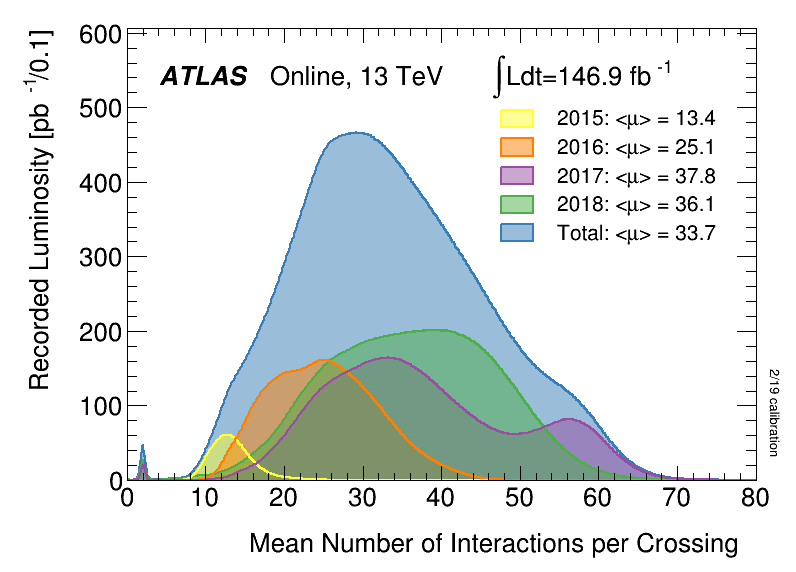
\includegraphics[width=0.75\linewidth]{figures/ExpSetup/PileupConditionsRun2.png}
% \caption{Pileup conditions throughout Run-2 \cite{LumiPublicResultsPage} \label{fig:expsetup:pileup}}
% \end{figure}

% %
% %\textcolor{gray}{
% %discuss accelerator chain - which energies in which accelerator 
% %some parts about magnet structure 
% %RF cavities for accelerations
% %include that the LHC is filled by single hydrogen bottle, its tilted to avoid water accumulating in the tunnel, magnet structure of the Lhc,  to focus beams and the RF cavities to accelerate.
% %}
% %.


% %include that the LHC is filled by single hydrogen bottle, its tilted to avoid water accumulating in the tunnel, magnet structure of the Lhc,  to focus beams and the RF cavities to accelerate.
% %Include some words on the bunch structure and the acceleration complex before the LHC. 
% %inlcude pileup discussion plot from lumi public results
% %integrated luminosity and instantaneous luminosity 
% %need to mention bunches, filling schemes to an extend, how often collisions are happening..
% %\textcolor{red}{have to mention what runs are - in connection with good runs lists}
% %\textcolor{red}{have to introduce run 1 and run 2 - because have run 1 analysis comparisons at some point? }
% %=====================================
% \FloatBarrier
% \section{ATLAS}
% \label{sec:ExpSetup:ATLAS}
% \FloatBarrier
% %=====================================
% The \ac{ATLAS} detector is located at Point 1 along the \ac{LHC}. This is the only \acs{CERN} site along the LHC ring with access to a main experiment, the \ac{SPS} as well as the LHC. 
% The overall structure is comparable to a barrel,  leading to the centre part of the detector being referred to as the barrel, as well as the large,  25m in diameter,  wheels on each side referred to as endcaps. 
% With its 25 meters tall and 44 meters length,  \ac{ATLAS} is the largest particle detector built on a collider so far. 
% It consists of multiple sub-systems and sub-detectors,  all built with different purposes in mind,  targeting momentum and energy reconstruction.  \ac{ATLAS} provides hermetic coverage around the beam axis,  enabling detection of all charged particles generated in the collisions in the plane orthogonal to the beam axis.  This is particularly important in searches for new physics, relying on analyses of momentum balances in the orthogonal plane such as discussed within this thesis.
% An illustration of the design of \ac{ATLAS} is given in Figure \ref{fig:expSetup:ATLASoverall}.  It is built up of multiple layers,  starting from the innermost component,  the \acf{ID},  providing tracking hits close to the beam pipe.  Surrounding the \ac{ID} is a system of two calorimeters. The outermost parts of \ac{ATLAS} are built by the muon spectrometer,  providing momentum reconstruction for muons passing through the inner detector layers. 
% Arguably one of the most striking features of \ac{ATLAS} is given through its magnet system.  Three superconducting Niobium-Titanium (NbTi) magnets span an overall length of 26m.  The first magnet system, the central solenoid,  is wrapped around the \ac{ID},  providing a 2 T axial magnetic field to curve the \ac{ID} tracks of charged particles. 
% The largest magnet parts are the eight barrel toroid coils,  intertwined with the outer muon system,  providing a total magnetic field of 4 T (0.5 T per coil) to measure the momentum of muons.  The toroid magnetic field is completed by the end-cap toroids,  also generating a magnetic field up to 4T for muons leaving \ac{ATLAS} close to the beam pipe. 

% \begin{figure}[htpb]
% \centering
% \includegraphics[width=0.9\linewidth]{../figures/ExpSetup/ATLAS_full.pdf} 
% \caption{Overview graphic of the ATLAS detector design \label{fig:expSetup:ATLASoverall},  with two people illustrated for scale reference \cite{ATLASfull}}
% \end{figure}

% Every component in \ac{ATLAS} working together enables the reconstruction and identification of a variety of particles with high precision.  An overview of the design capabilities of \ac{ATLAS} in terms of the momentum and energy resolution is given in Table \ref{tab:expSetup:Resolutions},  adapted from \cite{AtlasExperiment}.
% Here the resolution given lists first a stochastic term,  measuring the uncertainty based on the statistically dominated interaction of a particle with the material,  followed by a noise term,  which accounts for uncertainties due to electronic noise in the readout process. 

% \begin{table}[htpb!]
% \includegraphics[width=\linewidth]{figures/ExpSetup/ResolutionATLASDesign.pdf}
% \caption{Performance goals of the \ac{ATLAS} detectors' subsystems.  Units are given in GeV.  $\bigoplus$ indicating a sum in quadrature of the single terms for the total uncertainty \label{tab:expSetup:Resolutions}\cite{AtlasExperiment}. }
% \end{table}

% In the following, a brief overview of the detector is given; a more comprehensive description can be found in \cite{AtlasExperiment} as well as the Technical Design Reports of the subsystems,  as cited throughout the description below. 

% \subsection{ATLAS Coordinate system}
% The coordinate system used within \ac{ATLAS} is used throughout this thesis and shortly described in the following \cite{AtlasExperiment}. 
% The origin of the right-handed coordinate system is at the nominal interaction point,  with the positive x-axis pointing towards the centre of the \ac{LHC}.  The x-y plane is perpendicular to the beam axis,  defining the z-axis.  Towards the surface defines the positive y-axis.
% An azimuthal angle $\phi$ is defined around the beam axis, and a polar angle $\theta$ is the angle from the beam axis.  Instead of $\theta$ the rapidity $y$ is used for heavy objects:
% \begin{align}
% y = \frac{1}{2} \ln[(E+p_z)/(E-p_z)]
% \end{align}
% Differences in Rapidity are invariant under boosts along the beam axis.
% For massless objects or relativistic objects ($m << \vb*{p}$),  the pseudorapidity is used: 
% \begin{align}
% \eta = -\ln(\tan(\theta/2)) 
% \end{align}
% To quantify the distance between two objects,  $\Delta R$ is defined:
% \begin{align}
% \Delta R = \sqrt{\Delta\phi^2 + \Delta\eta^2} \label{eq:expsetup:deltaR}
% \end{align}
% The transverse momentum and energy are defined in the x-y plane,  with the transverse momentum given as $p_T = \sqrt{p_x^2 +p_y^2}$.

% %=====================================
% \subsection{Inner Detector}
% %=====================================
% A cross-section of the \ac{ID} system \cite{IDTDR} is shown in Figure \ref{fig:expSetup:InnerDetectors}, highlighting the distance of each subsystem from the beampipe. The innermost part of the \ac{ID}  is the \ac{IBL},  followed by three layers of pixel detectors.  At 299 mm radial distance from the beam pipe, four layers of \ac{SCT} modules are located before the \ac{TRT},  which extends the overall \ac{ID} detector size to a radius of 1082 mm.  The \ac{ID} allows for particle track reconstruction within $|\eta| < 2.5$.

% \begin{figure}[htpb!]
% \centering
% \subfloat[Sketch of the \ac{ID} and distances of its sub-detectors]{\includegraphics[width=0.49\linewidth]{figures/ExpSetup/ID_includingIBL.png}}
% \subfloat[Overview of barrel and end-cap \ac{ID} components, apart from \ac{IBL} \label{fig:expsetup:idendcaps}]{\includegraphics[width=0.49\linewidth]{figures/ExpSetup/ID_overview_noIBL.eps}}
% \caption{Slice view of the Inner Detector,  highlighting each sub-detectors distance to the beampipe \cite{IDsketchwithIBL} (a) and cut-out view of the barrel and endcap components,  not including the \ac{IBL} \cite{AtlasExperiment} (b).  \label{fig:expSetup:InnerDetectors}  }
% \end{figure}
% \paragraph{IBL - Insertable B-layer}
% After Run-1,  during a long shutdown in 2013-2014,  the pixel detector system was subject to maintenance and upgrades.  Within this set of upgrades,  %the \ac{DBM} was inserted within the pixel detector volume,  
% a 4th pixel layer at a 3.3 cm distance from a new,  smaller beam pipe (33 mm outer radius,  originally 36 mm).  A fourth pixel layer was a first in particle physics experiments \cite{IBLTDR,IBLproceedings} and has led to significant improvements in interaction vertex reconstruction and identification of b-hadron jets. 

% \paragraph{Pixel Detector}
% The innermost pixel layer,  the IBL,  is surrounded by three layers of pixel detectors,  arranged in barrels around the beam pipe \cite{PixelDesignPerformance,PixelPerformanceProceedings}.  The first layer is at a distance of 50.5 mm from the beam pipe's centre.  As can be seen in Figure \ref{fig:expsetup:idendcaps},  the end caps of the pixel layer consist of 3 disks around the beampipe,  stretching the length of the pixel component of the \ac{ID} to 1.4 m length along the beam axis.  The pixel detector consists of overall 1744 pixel modules with a nominal size of $50 \mu m x 400 \mu m$ in the $(\phi, z)$ plane ($\phi, r$ for the disk panels), comprising over 80 million readout channels.  
% The pixel and \ac{IBL} part of the ATLAS detector is crucial for tracking,  providing 4 pixel hits over the entire \ac{ID} pseudorapidity coverage ($|\eta| < 2.5.$).  
% %The resolution in the barrel is 10 mm (R-f) and 115 mm (z),as in the end-cap.

% \paragraph{Semiconductor Tracker}
% The pixel detector and \ac{IBL} are located within \ac{SCT} modules \cite{SCT}.  
% Similar to the pixel detector modules, the \ac{SCT} modules are semiconductor-based,  arranged into cylindrical layers around the beampipe in the barrel region,  forming disks in the endcap.  Since the \ac{SCT} modules only provide precise location along one axis,  two modules are combined back-to-back and rotated against each other to gain two dimensional spacial information.  Four layers are arranged in the barrel,  nine disks in each endcap side (see Fig. \ref{fig:expsetup:idendcaps}). Including the endcap disks, the \ac{SCT} extends up to $|z| < 2735 mm$. 

% \paragraph{Transition Radiation Tracker}
% The last part of the \ac{ID} is the \ac{TRT} \cite{TRTDesignPerformance},  in the barrel stretching from 554 mm to 1082 mm radial distance.  This detector is composed of 4 mm diameter straw tubes,  arranged in parallel to the beam pipe or radially in the barrel and end-cap, respectively.  Within $|\eta| < 2.0$,  three barrel rings and 18 end-cap units provide typically 36 hits per track. The straws are intertwined with polypropylene fibres for passing through particles to create transition radiation.  Inside the straws is a thin tungsten wire,  collecting charges drifting through the straws gas mixture (Xe, CO2 and O2). The level of radiation and collected charges in each straw can be used to discriminate between electrons and charged pions.  The \ac{TRT} only offers spatial information in the $(R-\phi)$ plane, no information in the z-direction can be extracted due to the straws orientation. 
 
% %70% Xe, 27% CO2 and 3% O2.
% %R − phi direction, while no information is provided
% %along the z-direction.
% %and can provide up to 36 hits per track.
% %up the TRT are straw tubes 4 mm in diameter,
% %with walls made of two multi-layer films, each 35  m thick.
% %The TRT is designed to provide a large number of hits, typically 36 per track,
% %with a coverage of j j < 2:0. It has an intrinsic accuracy of 130  m in R 􀀀  ,
% %providing no information in the z-direction
% %The TRT [71] consists of three barrel rings, with 32 modules each, and 18 end-caps units
% %31 2.2 The ATLAS detector
% %with 224 layers.
% %These are positioned
% %parallel to the beam pipe in the barrel and radial in the end caps. The
% %n the TRT this is done by polypropylene
% %fibres (foils), which are interwoven between the barrel (end-cap) straws, that enable
% %the production of transition radiation in the formof X-rays. The amount of radiation
% %produced can be used to distinguish between, e. g. electrons and charged pions, as the
% %amount of radiation would depend on how relativistic the charged particle is.

% %The TRT can discriminate between two signals, according to their
% %amplitude: the lowest charge is due to the minimum-ionising particles (MIPs) crossing the
% %gas, while the strongest signal is given by the transition-radiation photons absorbed in
% %the gas. This last class of events is originated by the electrons, hence the TRT is able to
% %contribute to electron identification on a straw-by-straw basis
% %\subsubsection*{SCT - Semiconductor Tracker }
% %\subsubsection*{TRT - Transition Radiation Tracker}
% %
% %gaseous/polypropylene-fibre transition radiation tracker (TRT) a
% %\subsubsection*{BCM - Beam Condition Monitor} --> beam condition monitor
% %\cite{BCM}
% %=====================================
% \subsection{Calorimeter System}
% %=====================================
% The overall \ac{ID} system is surrounded by two sets of calorimeters \cite{AtlasExperiment}.  An \acf{ECAL} \cite{LArTDR} in the inner most part, followed by a \ac{HCAL} \cite{TileTDR} (see Figure \ref{fig:expSetup:calorimeters}).  Both systems are designed to record the energy deposits of mainly electromagnetically interacting particles (electron,  photons) or the energy of hadrons,  based on hadronic interactions. 

% \begin{figure}[htpb!]
% \centering
% \includegraphics[width=0.75\linewidth]{figures/ExpSetup/Calorimeter_overview.eps}
% \caption{Illustration of the \ac{ATLAS} calorimeter system \cite{AtlasExperiment} \label{fig:expSetup:calorimeters}}
% \end{figure}

% Both calorimeters are so-called sampling calorimeters with alternating layers of absorber and active material.  The absorber layer triggers a shower development of consecutive interactions with the detector material,  the active layer is detecting the signal. The shower development and properties can be a helpful characteristic in particle identification.
% Overall,  the calorimeters cover the $|\eta|$ range below 4.9.  Two important quantities in connection with the calorimeters are the radiation length, $X_0$,  and the interaction length $\lambda$.   The radiation length  refers to the distance after which an electrons energy has been reduced to 1/e of its initial energy.  The interaction length describes the mean free path before the occurrence of an hadronic interaction.


% \paragraph{Liquid Argon Calorimeter}
% Liquid Argon (LAr) calorimeters \cite{LArTDR} are used in multiple parts of the calorimeter system.  First,  it is comprising the \ac{ECAL},  with two half barrels covering the central detector region, with a small (4 mm) gap at $z = 0$ and one end-cap on each side of the beamline (see Fig. \ref{fig:expSetup:ecal}).  Additionally,  the LAr technology is used for the hadronic calorimeters end-caps as well as a \ac{FCAL} ($3.1 < \eta < 4.9$). 
% The active material is LAr,  with copper and kapton electrodes for readout.  The absorber is made of lead with stainless steel sheets.  As can be seen in Figure \ref{fig:expSetup:ecal},  an accordion symmetry is used to ensure homogeneous coverage all over $\phi$.

% \begin{figure}[htpb!]
% \centering
% \subfloat[\label{fig:expSetup:ecal}]{\includegraphics[width=0.45\linewidth]{figures/ExpSetup/ECalVis.png}}
% \subfloat[\label{fig:expSetup:crack}]{\includegraphics[width=0.45\linewidth]{figures/ExpSetup/CrackRegionmaterial.png}}
% \caption{Visualisation of an \ac{ECAL} slice at $\eta = 0$ (a),   next to an overview of the material in terms of radiation lengths infront of the presampler and main \ac{ECAL} (b).  Both from \cite{AtlasExperiment}.}
% \end{figure}

% Infront of the \ac{ECAL} between $|\eta| < 1.52$ in the barrel region and $1.5 < |\eta| < 1.8$ in the end cap,  there is an additional layer of instrumented Liquid Argon,  the \textit{presampler}.  This is included in order to account for energy losses of particles before entering the \ac{ECAL}.  The first layer of the \ac{ECAL} has the finest granularity, comprising 4.3 $X_0$, followed by the second layer of 16 $X_0$ radiation lenghts in depth and a third layer with coarse granularity. 
% The total thickness in the barrel of the \ac{ECAL} is over 22 $X_0$,  over 24 $X_0$ in the endcap. 
% In Figure \ref{fig:expSetup:crack},  the amount of material infront of the presampler as well as the accordion part of the calorimeters is given in radiation lenghts.  Within the region of $ 1.37 < |\eta| < 1.52$,  a large amount of material is present.  This is due to the transition between the barrel and end-cap cryostats,  housing the calorimeters.  This region is knowns as the \textit{crack} region or transition region. 

% \paragraph{Tile Hadronic Calorimeter}
% The hadronic calorimeter is built of a tile calorimeter technology \cite{TileTDR} in the barrel and extend barrel region (between $0 < |\eta| < 1.7$,  see Figure \ref{fig:expSetup:calorimeters}).  Similar to the \ac{LAr} calorimeter the tile calorimeter is a sampling calorimeter,  with a steel absorber material as well as plastic scintillator tiles as active material.  The scintillator tiles are combined with optical fibres and photo-multipliers for signal readout.  In the barrel,  the tile calorimeter has an overall depth of roughly 9.7 interaction lengths. 

% %=====================================
% \subsection{Muon System}
% %=====================================
% The outermost part of the \ac{ATLAS} detector is the \ac{MS} \cite{MuonTDR}. It is embedded within the 4 T magnetic field generated by the barrel and endcap toroid magnets.  In Figure \ref{fig:expSetup:MS},  a quarter of the muon system is visualised, highlighting the different subsystems.  \acp{MDT} and \acp{RPC} form three layers around the barrel,  \acp{CSC} are used close to the beam pipe.  The \textit{Big Muon wheels},  forming the "lids" of the \ac{ATLAS} barrel structure,  are comprised of \ac{TGC} and \ac{MDT} subdetectors.  A short overview of the subsystems is given in the following.

% %d drift tube (MDT) and cathode strip (CSC) chambers for momentum determination an
% %resistive plate (RPC) and thin gap (TGC) chambers for triggering. The

% \begin{figure}[htpb!]
% \centering
% \includegraphics[width=0.8\linewidth]{figures/ExpSetup/MuonSpectrometer.png}
% \caption{Overview of a quarter of the muon spectrometer, showing all subsystems \cite{MuonTriggerPerformance} \label{fig:expSetup:MS}}
% \end{figure}

% \paragraph{MDT - Monitored Drift Tubes}
% The \ac{MDT} subdetectors of the muon spectrometer are drift tubes with a diameter of 29.97 mm.  They are filled with 93\% Ar,  7 \% CO2 and have a tungsten-rhenium wire in the middle.  There are in total 1171 \ac{MDT} chambers,  each layer with up to eight layers of drift tubes.  Overall 354240 tubes cover a pseudorapidity range up to $|\eta| < 2.7$,  providing high precision track coordinates perpendicular to the magnetic field.  In the innermost end-cap layer,  the \ac{MDT} chambers are replaced by \ac{CSC}'s. 

% %29.97 mm diameter drift tubes
% %93%Ar Å 7%CO2
% %tungsten-rhenium wire, measuring 50 ¹m in
% %Three to eight layers of drift tubes are used in
% %both barrel and end-caps to allow a total of twenty measurements for each track.\\
% %precision tracking
% %1171 MDT chambers, with a combined total of 354240 tubes.
% %ionisation
% %The coverage of the MDTs extends to
% %j j < 2:7 except in the innermost end-cap layer where they are limited to
% %j j < 2:0,
% %track coordinates
% %in the bending direction.
% %⌘| < 2.7.
% \paragraph{CSC - Cathode Strip Chamber}
% In the endcap in a pseudorapidity range of $2.0 < |\eta| < 2.7$,  the \ac{CSC} detectors provide a fast response and high spatial resolution,  similar to \ac{MDT}'s.  Since \ac{MDT} reach their maximum operational radiation tolerance close to the beampipe,  \ac{CSC} are used at the high radiation environment close to the beampipe.
% \ac{CSC} detectors are multiwire proportional chambers filled with the same gas mixture as \ac{MDT}'s.  They provide both $r$ and $\phi$ coordinates.
% %precision tracking
% %2:0 < j j < 2:7 replacing mdt's
% %incoming neutron
% %rate is expected to exceed 150 Hz=cm2, the maximum for safe operation of the
% %MDTs.
% %multiwire proportional chambers, using the same gas mixture
% %radial direction wire
% %characterised by a
% %fast response time and high spatial resolution
% %both radial and phi coordinate with
% Both \ac{MDT} and \ac{CSC} detectors are used for precision momentum measurements,  whereas \ac{RPC} and \ac{TGC} 
% detectors are used to provide fast information to the \ac{ATLAS} trigger system (see section \ref{sec:ExpSetup:trigger}).

% \paragraph{RPC - Resistive Plate Chambers}
% In combination with \ac{MDT}'s , \ac{RPC} detectors are used to provide a coarse,  quick,  secondary coordinate measurement.
% Each \ac{RPC} consists of two detector layers orthogonal to each other, providing $\phi$ and $\eta$ coordinate measurements.  The \ac{RPC} covers an overall pseudorapidity region up to $|\eta| < 1.05$.
% The detectors are named after the two resistive parallel plates of phenolic-melaminic plastic laminate within each chamber,  enclosing a gas mixture.
% %
% %triggering
% %provide a measure of the second coordinate in the
% %barrel.
% %They cover the pseudorapidity region |⌘| < 1.05.
% %much quicker response time compared
% %with the CSCs.
% %coarsely measure a second tracking coordinate in the
% %no-bending phi-projection to complement the
% %The chambers are filled with a gas mixture of C2H2F4 and a small fraction of resistive component
% %SF6 contained in two resistive parallel plates of bakelite, kept at a 2mm distance.
% %The two detector layers which form the chamber are placed orthogonally to read both the h and f
% %Two layers of chambers (middle station) provide the trigger for low-pT muons, while a
% %third one (outer station) is used for high pT trigger thresholds.

% \paragraph{TGC - Thin Gap Chambers}
% The last component of the \ac{MS} are \ac{TGC}.  They are multi-wire proportional chambers similar to \ac{CSC}'s,  but with a coarser granularity.  The gas filling is a mixture of CO2 and n-pentane (n-C5H12).  Similar to \ac{RPC} detectors,  \ac{TGC} are able to provide a signal faster than 25 ns,  allowing for a matchin of a signal to a specific bunch crossing.  Their fast readout time is used in the trigger system,  additional to \ac{MDT}, s they provide a secondary measurement of the azimuthal angle.   
% %triggering
% %TGCs are multi-wire
% %proportional chambers, filled with a mixture of CO2 and n-pentane (n-C5H12), and have a similar
% %structure as the CSCs but a higher granularity.
% %They are used as trigger chambers for muon tracks
% %and, in addition to the MDTs, they provide a second measurement of the azimuthal coordinate. Both
% %TGC and RPC chambers are designed to provide a signal over a time shorter than 25 ns.

% %=====================================
% %\subsection{Magnet System}
% %=====================================
% %\subsection{Forward Detectors}
% %%=====================================
% %%\subsubsection*{LUCID - Luminosity Cherenkov Integrating Detector}
% %%%\subsubsection*{AFP - ATLAS Forward Proton}
% %%\subsubsection*{ALFA - Absolute Luminosity For ATLAS}
% %%\subsubsection*{ZDC - Zero Degree Calorimeter}


% \FloatBarrier
% \subsection{The Trigger System}
% \label{sec:ExpSetup:trigger}
% %\subsubsection*{L1}
% %\subsubsection*{HLT}
% %\subsubsection*{MBTS - Minimum Bias Trigger Scintillator}

% With all the components of the ATLAS detector described above,  any interactions and electrical signals from the entire detector convolute into a large set of read-out information. Even without any proton-proton collisions provided by the \ac{LHC},  ATLAS can detect feedback from the detectors through for example cosmic muons. Storing every single interaction within ATLAS during collisions would exceed the storage capabilities of the CERN computing centres and simultaneous would not provide any differentiation between high energetic collision interactions and low energy scattering of the protons.
% The ATLAS trigger system has been designed to select collision events of interest to the multitude of physics analyses performed with ATLAS data.  To do so,  a two-stage trigger system was used during Run-2.  A visualisation of the trigger system, as well as the flow of data through this system, is given in Figure \ref{fig:expSetup:trigVis}.

% \begin{figure}[h]
% \centering
% \includegraphics[width=0.8\linewidth]{figures/ExpSetup/triggerSystem_withoutFTK.pdf}
% \caption{Overview of the ATLAS trigger system during Run-2.  Adapted from \cite{Run2TriggerOperation} \label{fig:expSetup:trigVis}}.
% \end{figure}

% The first trigger level is based in hardware.  This \textit{Level-1} trigger is built of processors digitizing the calorimeter readout and information from the muon spectrometers (\ac{TGC}, \ac{RPC}),  identifying electrons, photons,  tau leptons,  jets,  and can calculate missing transverse energy.  The L1Topo component of the Level-1 system allows for topological requirements such as invariant mass selections and distance measures to be taken into account in the Level-1 decision.  The final decision to keep or discard an event at Level-1 is made by the \ac{CTP}.  This Level-1 trigger step reduces the 40 MHz collision rate down to a maximum rate of 100 kHz \cite{Run2TriggerOperation} and passes on Regions-of-Interest in $\eta$ and $\phi$ to the next trigger step,  the \acf{HLT}.  Regions-of-Interest consist of neighbouring calorimeter cells in the \ac{ECAL} and \ac{HCAL},  a detailed discussion in connection with electron triggers is given in Chapter \ref{ch:trigger}.\\
% The \ac{HLT} is a software-based trigger,  a computing farm allowing for sequences of algorithms.  The \ac{HLT} is designed to reduce the event rate from 100 kHz to around 1 kHz that is saved.  The algorithms run on the \ac{HLT} farm have access to higher granularity calorimeter information as well as tracking information from the \ac{ID}.  A typical trigger sequence includes fast algorithms, designed to quickly reject events not targeted by the trigger,  followed by more precise algorithms that can run more time-consuming reconstruction and identification similar to events stored offline.  The exact sequence and type of algorithms considered at the \ac{HLT} are defined in the trigger \textit{menu}.  This comprises a database of triggers,  each trigger defining a sequence of algorithms and requirements on these algorithms for an event to pass the \ac{HLT}.  
% The overall set of triggers targeting various detector signatures associated with particles,  such as electrons,  muons or photons as well as missing transverse energy.  The trigger requirements are designed and budgeted in a way that the overall \ac{HLT} rate does not exceed 1 kHz. 
% In some cases,  even the reduction in event rate achieved through the \ac{HLT} algorithms for desired trigger requirements,  such as low momentum triggers,  is too high.  To keep the overall \ac{HLT} rate below 1 kHz in these cases,  triggers can still be included in the menu, but with a \textit{prescale}.  A prescale is an artificial scaling of the trigger,  only accepting every Nth trigger decision if the prescale factor is N.  This allows triggers with an otherwise high rate to still collect events.
% %\textcolor{red}{need to mention what trigger towers are}
% %\textcolor{red}{have mentioned the bandwidth and budgets of the different signatures? -- might have built up to this in the DAQ section}



\chapter{Data Acquisition,  Reconstruction and Monte Carlo Simulation}
\label{ch:DAQ}
\epigraph{\emph{“Champions keep playing until they get it right.”}}{Billie Jean King}

yet another template (yat)

% %\section{Data Aquisition}
% A crucial step in the recording of collision events with ATLAS is the selection through dedicated signature triggers.  These trigger decisions are emulated in Monte Carlo simulation in order to replicate the selection in data.  
% After events have been selected by the ATLAS trigger system and saved to disk,  further detailed reconstruction and identification algorithms can be performed.  In the following,  a short overview of the signature triggers of importance to this thesis as well as a summary of the reconstruction and identification processes for the particles and physics objects used in this thesis is given. 
% Additionally,  a brief description of Monte Carlo concepts and ATLAS detector simulation is given.

% \section{Signature triggers}
% \label{sec:DAQ:SignatureTriggers}

% %have to include a discussion about prescaled triggers, unprescaled triggers as well as RERUN triggers! also be clear what a trigger chain is! 
% %need to talk about trigger 'budget' or how the rate reduces from step to step,  e.g. referring to trigger budget of 1kHz at the HLT  in the trigger chapter
% %have to mention isolation in the electron trigger chain case
% An introduction to the ATLAS trigger system was given in section \ref{sec:ExpSetup:trigger}; in the following an overview of the trigger signatures of importance to this thesis are discussed.
% All the trigger signatures combined form a \textit{trigger menu},  a selection of triggers  simultaneously active in ATLAS in order to select all events of interest to the multitude of physics analyses in the ATLAS collaboration. 
% A trigger is a unique identifier for a sequence of trigger algorithms and the requirements that have to be fulfilled after each algorithm step,  including a specification of the Level-1 hardware trigger requirements.  A signature here refers to the combination of specific interactions that different \ac{SM} particles have with the various ATLAS detector layers.  

% %\begin{figure}[htpb!]
% %\centering
% %\includegraphics[width=0.6\linewidth]{figures/DAQ/TrigOpsPublicWinter2019_HLT_group_rates_ATLASStyle_359872.pdf}
% %\caption{Exemplary overview of physics stream trigger rates at the \ac{HLT} as a function of time.  \label{fig:DAQ:TriggerBudget}}
% %\end{figure}

% %Taken from \textit{https://twiki.cern.ch/twiki/bin/view/AtlasPublicTriggerOperationPublicResults#Trigger_rates_and_bandwidth}

% \subsection{Electron triggers}
% The electron trigger signature uses signals from the electromagnetic and hadronic calorimeters at Level-1 to select high energetic clusters of calorimeter towers.  Based on that decision,  a fast selection,  followed by precision algorithm-based selections at HLT are performed.  Very detailed work on the electron trigger has been part of the PhD work of the candidate,  therefore  a detailed discussion of the electron trigger signature as well as its performance in Run-2 is discussed in chapter \ref{ch:trigger}.
 
% \subsection{Muon triggers}
% The muon trigger signature relies on signals from the \ac{MS} and tracks from the \ac{ID}.  
% In the Barrel of the detector,  the Level-1 muon trigger signal consists of coincidences of hits in two or three \ac{RPC} segments for high and low $p_T$ momentum muons,  respectively.  
% In the End-Cap region ($1.04 < \abs{\eta} < 2.4$),  the  Level-1 muon decision is based on coincidences in the \ac{TGC} segments of the Big Muon Wheel.  After this first Level-1 step,  information on \ac{ID} tracks is accessible at \ac{HLT}.  
% Multiple isolation requirements on the muons at trigger level can be applied. 
% The lowest unprescaled single muon trigger uses a lower momentum threshold of 20 GeV in 2015,  raised to 26 GeV from 2016 onwards.  The efficiency of the lowest unprescaled single muon trigger between 2016 and 2018 is shown in Figure \ref{fig:DAQ:muontrigger}.  
% An extensive description of the muon trigger and its performance in Run-2 can be found in \cite{MuonTriggerPerformance},  here only a short overview can be given.
% The efficiency of the trigger is calculated on recorded collision events with selections targeting events with Z-bosons decaying into a opposite-sign di-muon final state.  A selection of muons from this decay,  is used as unbiased \textit{probe} sample to test the trigger's selection efficiency.  The trigger efficiency is defined as a ratio of the selected probe muons fullfilling the trigger selections over all available probe muons. The trigger in Figure  \ref{fig:DAQ:muontrigger} shows a fast turn-on of its efficiency in dependency of the probe muon's momentum,  reaching almost 70\% efficiency in the barrel regions and 90\% in the detector end-caps,  with a close agreement between data and Monte Carlo simulation visible in the lower panels.   
% \begin{figure}[h]
% \centering
% \includegraphics[width=0.95\linewidth]{figures/DAQ/MuonTrigger.png}
% \caption{Efficiency of the lowest unprescaled muon trigger in data collected between 2016 and 2018 in the detector barrel ($|\eta| < 1.05$) and end-cap ($1.05 < |/eta| < 2.5$) regions\label{fig:DAQ:muontrigger}, from \cite{MuonTriggerPerformance}}
% \end{figure}
% The lower trigger efficiency observed in the barrel region compared to the end-cap is due to a smaller geometric coverage at the Level-1 trigger stage.  

%  \subsection{Missing transverse momentum triggers}

% Missing transverse energy (\Met) in the detector is one of the essential features in many \ac{BSM} searches in ATLAS.  In connection with R-parity conserving \ac{SUSY},  the lightest neutralino particle is stable and can escape the detector without being detected. 
% This detector signature is similar to neutrinos escaping the detector. 
% Triggering on missing transverse momentum in this thesis is used in combined triggers with taus.
% The \MET  trigger is solely based on calorimeter information; multiple algorithms are available on the High-Level-Trigger to calculate the missing transverse momentum,  varying in the definition of used calorimeter clusters and their calibration.
% In essence,  a projection and summation of the clusters as described in equation \eqref{eqn:daq:met} \cite{MetTrigger} is performed.  
% \begin{align}
% \begin{split}
% E_x^\text{miss} = - \sum_{i=1}^{|\text{Elements}|} E_i \sin\theta_i \cos\phi_i\\
% E_y^\text{miss} = - \sum_{i=1}^{|\text{Elements}|} E_i \sin\theta_i \sin\phi_i
% \label{eqn:daq:met}
% \end{split}
% \end{align}
% A detailed explanation of the \MET trigger and its performance in Run-2 can be found in \cite{MetTrigger}.  For data analysis and selection discussed in this thesis,  only the most rudimentary missing transverse energy \ac{HLT} algorithm is used.  This is extracting \Met from a sum of all calorimeter cells with their uncalibrated energy above a noise threshold.  This noise threshold is included to avoid electronic noise and pile-up contributions.

%   \subsection{Tau Triggers}
%   \label{sec:daq:tautriggers}
% The tau trigger signature is based on a fast selection of electromagnetic and hadronic clusters at Level-1,  followed by reconstruction and identification algorithms run at the \ac{HLT}.  A detailed description can be found in \cite{TauTrigger}; a summary is given below.\\
% The applied selections are based on hadronic tau decays happening before traversing the active detector region. These signatures are showing as narrow calorimeter energy deposits with a small number of associated tracks. 
% At ~Level-1, ~ a core region made of $2\times2$ trigger towers ( each $0.1 \times 0.1$ in $\Delta\phi \times \Delta \eta$) is defined, with the $E_T$ of the hadronic tau candidate made up of the two most energetic consecutive cells. 
% Around this core region, an isolation region of $4\times4$ trigger towers is used to determine the isolation in the electromagnetic calorimeter. 

% The tau energy reconstruction at Level-1 does not include any calibrations or clustering algorithms and has a worse energy resolution than observed in the offline tau reconstruction. This leads to a signal efficiency loss for low transverse energy tau candidates.
% Regions-of-Interest selected by the Level-1 are passed to the HLT. 
% The tau selection here includes three steps: a calorimeter only selection, a track preselection, and an offline-like selection. 
% The calorimeter-only selection step uses the full detector granularity,  making use of the topological clustering algorithm \cite{TopoClusters}. This algorithm,  generating so-called \textit{Topo-Clusters} considers the significance of the electronic signal of each calorimeter cell and removes calorimeter cells if they are not close to cells with a large signal.  This topological clustering includes information about the shape and location of the cluster, allowing for calibrations to be applied.  In the tau trigger case described here,  a simplified tau energy calibration is applied. 
% The track preselection step makes use of a two-stage fast-tracking reconstruction. 
% At first, tracks within a narrow area along the beam axis are reconstructed, finding the tau vertex. In a second step, tracks in a larger $\Delta R$ window are considered, but in a narrow interval around the tau vertex. 
% This allows for fast reconstruction of the vertex and significantly reduces the CPU usage compared to a reconstruction of tracks in a large $\Delta R$ and z window.
% Eventually,  an offline-like selection is applied. 
% The tracks reconstructed in the previous step are now passed through precision tracking and therefore available with higher accuracy.  Together with the calibrated clusters,  multiple kinematic variables are used as input to a Boosted Decision Tree. This \ac{BDT} is similar to an identification method previously used to identify offline taus.  The \ac{BDT} is trained to distinguish taus from jets, using features such as the maximum distance in $\Delta R$ of the tracks associated to the tau,  with tracks associated with jets expected to be more wide-spread than tau associated tracks.  A detailed description of the \ac{BDT} can be found in \cite{TauRecoBDT}. %fix this reference: https://cds.cern.ch/record/2064383
% Multiple tau identification working points are defined based on fixed cuts on the \ac{BDT} output score.  At trigger level,  a medium working point is used. 
% %To allow for low tau pt thresholds, an additional requirement at level  1 must be made.  L1Topo is used to ask for an additional jet in the event. This is necessary to lower the trigger rates. 

 
%  \section{Object Reconstruction}
%  \label{sec:DAQ:ObjectReco}
% After the selection of events through the signature triggers described above,  the particle signatures are reconstructed and identified \textit{offline},  after they have been saved to storage.  This reconstruction is done event by event with the same procedure applied to Monte Carlo simulation and recorded ATLAS data. 
% Each particle has its reconstruction and identification procedure and can have additional algorithms to help with the specification of its properties.  Since the event is already recorded,  less limitations on the CPU consumption and timing constraints governing the online reconstruction can be used. 
% In the following,  a brief overview of the offline reconstruction and identification of the objects used in this thesis is given. 

% \subsection{Electrons}
%   \label{sec:DAQ:ObjectReco:Electrons}
 
% The main features of an electron or positron (in the following both referred to as electron) in ATLAS is a cluster of energy deposits in the \ac{ECAL},  tracks in the \ac{ID}  as well as a close match between the clusters and tracks in terms of $\eta \times \phi$.
% These three main features present the three consecutive steps in reconstructing electrons: first,  a seed cluster is reconstructed: Based on a sliding-window algorithm,  looking at collections of energy towers with at least 2.5 GeV of summed transverse energy. 
% Here an energy tower is the sum of collected energy in all three layers of the \ac{ECAL},  including the presampler,  in a $\Delta \eta \times \Delta \phi = 0.025 \times 0.025$ segment. This mimics the granularity of the second layer of the \ac{ECAL}.
% In Figure \ref{fig:DAQ:egammareco},  the path of an electron through the different detector components is illustrated,  also highlighting the three different layers in the \ac{ECAL}.

% \begin{figure}
% \centering
% \includegraphics[width=0.8\linewidth]{figures/DAQ/EgammaReco.png}
% \caption{Illustration of an electron path through the Inner Detector and Calorimeters of ATLAS,  highlighting the layer granularity in the electromagnetic calorimeter.  The dashed line presents a photon produced through interactions of the electron with the \ac{ID} material. Taken from \cite{ElectronRecoID1516}. \label{fig:DAQ:egammareco}}
% \end{figure}

% After the seed cluster is identified,  tracks are reconstructed.  This is based on pattern recognition of hits in the \ac{SCT} and Pixels,  followed by an ambiguity resolution step,  resolving ambiguity of hits associated with multiple tracks, and an extension of the tracks to the \ac{TRT}.
% For the fitting of tracks,  a global $\chi^2$ fitting procedure is used,  with either a pion hypothesis or an electron hypothesis in the presence of significant Bremsstrahlung. 
% Consecutively,  a \ac{GSF} \cite{GSF} is applied to account for energy losses in the \ac{ID} material. 
% As the last electron reconstruction step,  a matching of the GSF-track and calorimeter cluster is performed.  This matching is based on a geometric distance between the clusters and tracks and is described in detail in \cite{ElectronRecoID1516}.  The electromagnetic energy clusters are further calibrated as described in \cite{ElectronCalib}.

% After the reconstruction,  a further identification is necessary to distinguish prompt electrons from electrons originating from misidentified hadrons, non-isolated electrons from heavy-flavour decays or electrons from photon conversion. 

% This identification is based on a likelihood discriminant construction.  The likelihood discriminant $d'_L$ is given in equation\eqref{eqn:daq:eleclikelihood} \cite{ElectronRecoID1516},  where a fixed factor $\tau = 15$ is used to achieve a smooth discriminant distribution.   

% \begin{align}
% \begin{split}
% d_L &= \frac{L_S}{L_S + L_B} \\
% d'_L &= -\tau^{-1} \ln(d^{-1}_L -1)
% \label{eqn:daq:eleclikelihood}
% \end{split}
% \end{align}

% Here $L_S$ describes the likelihood function of signal,  prompt electrons. Whereas $L_B$ is the likelihood of non-promt,  fake electrons.  The likelihoods $L_S$ and $L_B$ are a product of probability density functions for a large set of kinematic variables.  The distributions and the likelihoods are binned in the $p_T$ and $\eta$ of the electron candidate.  A complete set of the variables considered in the likelihood definition is included in \cite{ElectronRecoID1516}, as well as a detailed description of the pdf and likelihood extraction.  
% Using a multi-variate technique can help where a simple cut on single variables would not offer strong discriminating power.  
% %based on discussion and drafting with Stefan Richter! 
% Based on the output of the discriminant,  several working points are defined.  These are designed to have a given signal-electron selection efficiency in each $(p_T, \eta)$ bin. Therefore a cut on the discriminant is defined in each $(p_T, \eta)$ bin.  In addition, to stabilise the performance at high pileup (to avoid getting too much increase in background passing the selection),  the cut on the discriminant is done such that it depends linearly on a pileup variable.  
% %in each $p_T-\eta$ bin i
% Effectively,  the cut gets tightened as pileup increases.  The number of primary vertices in the event is used as the pileup variable for offline electrons.  For online electrons, this is too computationally intense, so the number of inelastic collisions per bunch crossing ($\mu$) is used instead as a measure of the amount of pileup.
% Additional to the electron likelihood based identification,  isolation requirements can be applied to distinguish between prompt electrons and electrons from heavy-flavour decays.  Two isolation criteria for offline electrons are defined,  \textit{FCTight} and \textit{FCLoose}.  These isolation working points include a restriction on the transverse energy sum in a $\Delta R <0.2$ region around the electron in the calorimeter ($E_T^\text{iso}$) to be below 0.06 and 0.2 times the electrons energy ($E_T$), for \textit{FCTight} and \textit{FCLoose}, respectively.  The calorimeter based isolation requirement is combined with a track-based isolation, restricting the momentum.  The radial distance has a maximum value of 0.2 and decreases with the electrons momentum.  For the \textit{FCTight} working point,  the momentum fraction within the isolation cone is restricted to be smaller than  0.06 times the electrons momentum,  for \textit{FCLoose} it is below 15\% of the electrons momentum. 
% %pileup distr in each pt eta bin - schnitt auf disk linear function of pileup dependency
% %id menu dep pt eta and pileup 
% %disc schnitt (Y) pileup (X) - steigung konstruiert 0 very loose , tight am stärksten - damit tight immer medium erfüllt und es nicht vorkommen kann dass tight für hohes pileup medium nicht erfüllt

  
%   \subsection{Muons}
% Muon candidates as minimum ionising particles in ATLAS are reconstructed using track segments from the Muon Spectrometer that have been matched to \ac{ID} tracks.  Energy loss in the calorimeters is taken into account in a combined fitting of \ac{MS} and \ac{ID} tracks.  
% Multiple identification working points in varying levels of prompt muon selection efficiency and background rejection are defined,  designed to satisfy the large varying needs of physics analyses.  Additional to identification criteria,  an isolation requirement can be applied \cite{MuonID}.  Similar to the electron isolation working points,  a muon isolation based on calorimeter and track-based isolation criteria is defined,  \textit{FCLoose}.  The transverse energy in a  $\Delta R < 0.2$ isolation cone around the muon is restricted to 30\% of the muons momentum.  Addtionally, the momentum in a variable size, maximum $\Delta R < 0.3$ cone around the muon should not extend 15\% of its momentum. 

% \subsection{Jets}
% The particle-flow jet reconstruction \cite{ParticleFlow} makes use of calibrated Topoclusters as well as tracking information from the \ac{ID}.  The topological clustering algorithm has been previously introduced and discussed in section \ref{sec:daq:tautriggers} in relation to tau triggers. The anti-$k_T$ sequential recombination algorithm \cite{antikt} is used to form jet objects based on particle-flow objects.  To remove pile-up jets,  a multivariate discriminant based on vertex information,  the \ac{JVT} \cite{JVT} can be used.

% %topological clusters of calorimeter cells 

% \subsection{Taus}
% \label{sec:DAQ:ObjectReco:Taus}
% As briefly highlighted within the description of the tau trigger in section \ref{sec:daq:tautriggers},  hadronic tau decays have a distinct detector signature that can be used to trigger on events containing hadronic taus.  In the following,  a brief discussion of the tau decay is given to provide a baseline of the features important to this thesis, before summarizing the hadronic tau reconstruction and identification within \ac{ATLAS}.
% Tau leptons have a mass of $1776.86  \text{ MeV}$ and a mean lifetime of $290.3 \times 10^{-15} \text{ s}$ \cite{PDG2022}. With their proper decay length around $87 \mu\text{m}$ \cite{PDG2022},  taus decay before interacting with active detector layers of \ac{ATLAS}.  As can be seen in Figure \ref{leptaudecay},  tau leptons decay via a $W$ boson and a tau neutrino.  The hadronic or leptonic decay of the tau is determined through the consecutive decay of the $W$-boson,  Figure \ref{leptaudecay}, highlighing a leptonic decay into an electron. Leptonic decays of the tau make up 35\% of tau decays, with hadronic decays making up 65\% \cite{PDG2022}.  Examples of hadronic tau decays are given in Figure \ref{hadtaudecay},  highlighting the calorimeter systems in which the decay products will leave the majority of their energy.  Not explicitely shown in the sketch is the $W$-boson,  only its decay products.  In 72\% the hadronic tau decay includes one charged pion,  in 22\% of the cases the decay includes three charged pions.  These charged pions leave tracks in the \ac{ID},  presenting a distinct identfication feature of taus,  the number of charged tracks or \textit{prongs} associated with their decay. 
% %t 65% of all possible decay modes [1]. In these, the hadronic decay products are one or three charged pions in 72% and 22% of
% %all cases, respectively. 
% The hadronic decay of a tau lepton is determined through the quarks and intermediate mesons built in the $W$-boson decay.  Examples thereof are shown in Figure \ref{hadtaudecay}. 
% \begin{figure}[h]
% \subfloat[\label{leptaudecay}]{\includegraphics[width=0.25\linewidth]{figures/tauLep.pdf}}
% \subfloat[\label{hadtaudecay}]{\includegraphics[width=0.7\linewidth]{figures/taudecay.pdf}}
% \caption{Feynman diagram of a leptonic tau decay,  highlighting its decay via a W-boson (a). Examples of hadronic tau decays into (from left to right) one charged pion,  one charged and one neutral pion as well as three charged pion (b)\cite{TauDecayTikz},  highlighting in which detector systems the participating particles will be detected.  \label{taudecay}}
% \end{figure}

% Hadronic tau candidates are seeded from jets that have been reconstructed using the anti-$k_T$ algorithm,  with a distance parameter of $\Delta R =0.4$  \cite{TauReconstruction}.  Additionally,  jet seeds are required to have $p_T > 10 \text{ GeV}$ and $|\eta| <2.5$.
% %A tau vertex is identified among all primary vertex candidates that lies within $\Delta R < 0.2$ of the jet axis.
% A \ac{BDT} is used to categorize all tracks associated to the tau candidate within $\Delta R = 0.4$ of the tau axis to be core or isolation tracks.  The number of core tracks is used to define the prongness of taus,  indicating the number of charged particles involved in the tau's decay.

% To distinguish tau particles from jets,  a recurrent neural network (RNN) identification is used.   
% For this,  multiple kinematic variables are used for the training of an RNN \cite{TauRNNID}.    
% Variables include specifications of the cluster depth, the longitudinal extension and the radial cluster extension as well as fractions of momenta in the core or isolation region of the tau cluster,  to highlight a few of them. 
% The performance of the RNN identifier is shown in Fig. \ref{fig:DAQ:tauPerformance} for its 1-prong and 3-prong decay modes. This is also compared with the performance of a BDT identifier previously used in the $\tau$ identification in ATLAS.  The improved network architecture of the RNN identifier provides  rejection of jets by up to a factor of two better than the previous BDT approach. 

% \begin{figure}[h]
% \centering
% \includegraphics[width=0.6\linewidth]{figures/DAQ/RNNPerformance.png}
% \caption{Performance of the tau \ac{RNN} identification working points in comparison with previously used \ac{BDT} based identification \label{fig:DAQ:tauPerformance} \cite{TauRNNID}}
% \end{figure}

% \subsection{Missing transverse energy}
% The reconstruction of missing transverse energy after an event has been stored by a trigger is similar to the procedure at trigger level described in section \ref{sec:DAQ:SignatureTriggers}.  In contrast to the trigger reconstruction,  the offline missing transverse energy reconstruction is not based on uncalibrated clusters, but fully calibrated physics objects.  Additionally to this part of the \Met reconstruction considering physics object,  a soft term comprised of low momentum tracks is taken into account \cite{MetPerformance}.

% \section{Monte Carlo Simulation}
% \label{sec:DAQ:MC}
% To evaluate any measurements taken with the ATLAS detector,  simulations of physics processes and their decay within the ATLAS detector are necessary.  This is achieved through the use of Monte Carlo event generators.  In the following,  a brief description of the essentials of Monte Carlo simulations are given,  based on pedagogic introductions given in \cite{MCPedagogic}.  Followed by a short overview of the Monte Carlo generators used in this thesis.
% For the production of a final state X through the collision of two hadrons ($h_1$, $h_2$),  the inclusive cross section can be factorised like the following:

% \begin{align}
% \sigma_{h_1,h_2\rightarrow X} = \sum_{a,b\in {q,g}} \int dx_a \int dx_b f_a^{h_1}(x_a,\mu_F^2)f_b^{h_2}(x_b, \mu_F^2) \int \,d\Phi_{ab\rightarrow X} \frac{d\hat{\sigma}_{ab}(\Phi_{ab\rightarrow X},\mu_F^2)}{\,d\Phi_{ab\rightarrow X} }
% \label{eq:DAQ:xsec}
% \end{align}
% With $f_a^{h_1}(x_a,\mu_F^2)f_b^{h_2}(x_b, \mu_F^2)$ representing the parton distribution functions. 
% Here $\mu_F$ presents the factorisation scale.  This scale is the cutoff between processes that are considered perturbatively and the non-perturbative regime.  
% %In order to evaluate the systematic uncertainty caused by the cross section's dependence on the factorisation scale,  this scale is varied in alternative samples.
% An important part of this inclusive cross section is presented by the Matrix element describing the hard scattering process,  this is included in the last integral of equation \eqref{eq:DAQ:xsec}.
% After the inclusive matrix element calculation as described in equation \eqref{eq:DAQ:xsec},  the parton showering takes into account the additional particles that can contribute to the production.  The parton showering here is considering that a parton can originate from a splitting of  other partons.
% To not consider the additional particles twice,  a matching of the matrix element and the parton showering has to be performed.  
% The produced partons in such a showering will form colourless hadrons,  which in turn can further decay.  A last aspect to be taken into consideration for event simulations is the underlying event. This is caused by \textit{spectator} partons, not directly participating in the hard scattering.


% \subsection{Monte Carlo generators}

% \paragraph{Sherpa}
% One of the general purpose event generators used in this thesis is \texttt{SHERPA} \cite{Sherpa}.  It includes matrix element generators as well as a built-in parton showering.  In this thesis,  simulated events with \texttt{SHERPA} include Multi-boson processes as well as the associate production of vector bosons and jets.  

% \paragraph{Powheg} 
% The \texttt{POWHEG} \cite{Powheg} framework is a matrix element generator at next-to-leading perturbative order.  The matrix element generation is interfaced with generators like \texttt{PYTHIA} or \texttt{HERWIG++} in order to simulate the parton shower.  This kind of combination of matrix element generator and parton shower simulation is used or top-related processes such as top-antitop pair production. 

% \paragraph{MadGraph5\_ aMC@NLO} \texttt{MadGraph5} \cite{Madgraph} is used as a matrix element calculator at next-to-leading perturbative order.  Similar to \texttt{POWHEG},  it is interfaced with \texttt{PYTHIA} or \texttt{HERWIG} to include parton showering. 

% \paragraph{Pythia}
% A second general purpose event generator used in this thesis is \texttt{PYTHIA 8}\cite{pythia},  even with matrix element calculation and parton showering possible within \texttt{PYTHIA}, it is widely used for its parton showering,  interfaced with \texttt{POWHEG} or \texttt{HERWIG}.  Additionally,  \texttt{PYTHIA} is used in this thesis to simulate minimum-bias proton-proton collisions.

% \paragraph{Herwig} The \texttt{HERWIG} \cite{Herwig,Herwig++} Monte Carlo event generator has capabilities to be used to simulate the matrix element,  but is only used within this thesis as a variation of the \texttt{PYTHIA} parton showering. 

% \paragraph{EvtGen}
% \texttt{EvtGen} \cite{EvtGen} is a framework that simulates the decay of final state particles.  Events associated with the production and decay of a top quark used in this thesis are simulated through a combination of \texttt{POWHEG}, \texttt{PYTHIA} and \texttt{EvtGen}.  Within this thesis, all events generated with a parton showering by \texttt{PYTHIA} include final state particle decays simulated with \texttt{EvtGen}.

% \subsection{ATLAS detector simulation}
% \label{sec:DAQ:AF2}


% To directly compare the data collected with the ATLAS detector with the prediction of \ac{SM} and \ac{BSM} events in simulation,  the interaction of the produced particles with the detector material has to be simulated.
% The Geant4 \cite{Geant4} software package is used to simulate the interaction of particles with the detector material.
% A full Geant4 model of the ATLAS detector is used to simulate the transition of particles produced in proton-proton collisions through the different detector layers. 

% The simulation of a large number of interactions necessary to mimick the ATLAS reconstruction is computationally extensive.  Especially the simulation of shower developments in the calorimeters consumes a large amount of CPU and computing time. 
% For many \ac{BSM} searches,  a large number of parameters affecting the predicted particle masses and interactions have to be simulated.  A 'fast' parameterised detector simulation has been developed to cope with this high simulation demand.  A so-called Atlfast-II or AFII setup simulation chain uses Geant4 simulation for the interactions in the \ac{ID} and muon spectrometer,  but a parametrised simulation called FastCaloSim for the particle interactions in the electromagnetic and hadronic calorimeter. 
% The improvements in computing time compared to Geant4 simulation of the full detector as well as a fast,  simplified Geant4 simulation is shown in Figure \ref{fig:DAQ:AFIIvsG4}.  The overall processing time is reduces by roughly an order of magnitude compared to the full Geant4 simulation \cite{AFIIprinciple}. 
% \begin{figure}[h]
% \centering
% \includegraphics[width=0.8\linewidth]{figures/DAQ/AFII_CPU_improvement.png}
% \caption{CPU time distributions for 250 $ \ttbar $ events compared for G4,  fast G4 and AFII setup,  taken from \cite{AFIIprinciple} \label{fig:DAQ:AFIIvsG4}}
% \end{figure}
% The fast calorimeter simulation FastCaloSim uses a parametrisation of the calorimeter response.  The parametrisation has been extracted through Geant4 simulation and tunes to data. 
% The main three simplifications include simplifying the detector geometry,  approximating the calorimeter cells as cuboids,  only reproducing the average lateral energy distributions and restricting the simulation to three types of initial particles. 





\part{Search for resonances}
% \input{Chapters/5_reconstruction}
% \input{Chapters/6_reconstruction}
% \input{Chapters/7_reconstruction}
% \input{Chapters/8_reconstruction}



\FloatBarrier


%  \chapter{The ATLAS Electron Trigger Performance in Run-2}
\label{ch:trigger}
%\epigraph{\emph{'Don't let anyone rob you of your imagination, your creativity, or your curiosity. It's your place in the world; it's your life. Go on and do all you can with it, and make it the life you want to live.'}}{Mae Jemison}
\epigraph{\emph{My mission in life is not merely to survive but to thrive and to do so with some passion, some compassion, some humor, and some style.}}{Maya Angelou}
%\epigraph{\emph{'I didn’t want to just know names of things. I remember really wanting to know how it all worked.'}}{Elizabeth Blackburn}
%\textcolor{red}{double check whether the single electron trigger in 2015 actually didn't have an e60 chain in it! make sense because it is already lhmedium, but check!}\\ --> have calculated this in the confg with the e60 chain, but effectively not gaining any efficiency benefits through it - so the official single electron OR does not include it here - its the same efficiency but shifted to higher et turn on - ignore the e60lhmedium chain 
The following chapter gives an introduction to the electron trigger in ATLAS and describes the performance of selected electron triggers during Run-2.  This work is part of the author's involvement in the ATLAS electron and photon trigger signature group between 2018-2022.  The main focus of this work is the measurement of trigger efficiencies as well as the calculation of trigger scale factors,  which have been widely used in physics analyses of the Run-2 dataset.
This work has contributed in a major way to the first electron and photon trigger performance publication in ATLAS \cite{TrigEgammaPaper} and has been presented by the author at the ICNFP2019 conference \cite{ICNFPtalk, ICNFPProceedings}.  \\
In section \ref{sec:trigg:Intro},  an introduction to the electron trigger signature is given,  followed by a discussion and motivation of the electron trigger menu in section \ref{sec:trigg:Menu}.  A brief explanation of the efficiency and scale factor calculation methodology is given in section \ref{sec:trigg:methodology}. The trigger performance throughout Run-2 including full Geant4 detector simulation (section \ref{sec:trigg:fullsimPerformance}) as well as parametrised AF2 simulation (section \ref{sec:trigg:fastsimPerformance}) is then completed by a short discussion on the perspectives and limitations of these studies in section \ref{sec:trigg:perspectives}. 
\section{The ATLAS electron trigger}
\label{sec:trigg:Intro}
Triggers selecting electron signatures are widely used in ATLAS.  They target a detector signature of tracks in the \ac{ID},  combined with energy deposits in the \ac{ECAL}.
As described in section \ref{sec:ExpSetup:trigger},  the first selection step for any signature is the Level-1 trigger.  For electrons,  this consists of clusters in the electromagnetic calorimeter.  The Level-1 trigger identifies a \ac{RoI},  a group of neighbouring trigger towers.  A trigger tower presents a sum of calorimeter cells in a $\Delta \eta \times \Delta \phi$ region in the detector,  including the various layers in the \ac{ECAL} and \ac{HCAL}.  As can be seen in the visualisation given in Figure \ref{L1Vis},  this Region-of-Interest is the local maximum of transverse energy deposited in the calorimeter cells.  A specified energy threshold is passed at Level-1 if any of the 2x1 or 1x2 connected trigger towers in the \ac{RoI} exceed the specified threshold.  The trigger towers have a granularity of $\Delta \eta \times \Delta \phi = 0.1 \times 0.1$ \cite{TriggerSystem2015}. The energy of the clusters has undergone a electromagnetic energy scale calibration.  This calibration reconstructs the energy deposited through an electromagnetic shower,  but is not able to correctly account for energy losses in hadronic shower developments.  An energy threshold variable in $\eta$ around a nominal $E_T$ threshold can be applied,  accounting for geometrical dependencies in the energy cluster calibrations.  Illustrated through a bright yellow ring in Figure \ref{L1Vis},  a requirement on the isolation of the core can be made. This sets a limit on the sum of transverse energy contained in the 12 trigger towers surrounding the Region-of-Interest,  in comparison to the energy contained in the core.  Lastly,  a limit on the hadronic leakage can be required.  This limit restricts the energy contained in the hadronic calorimeter trigger towers behind the central 2x2 clusters in the electromagnetic calorimeter.
Any requirements on the hadronic leakage or isolation are only applied to transverse energies reconstructed at Level-1 below 50 GeV \cite{TrigEgammaPaper}.

\begin{figure}[htb!]
\centering
\includegraphics[width=0.4\linewidth]{figures/TrigEgamma/EGammaTauAlgo.pdf}
\caption{Visualisation of the Level-1 electron selection \cite{TriggerSystem2015} \label{L1Vis}}
\end{figure}

The selections required from the Level-1 trigger form the basis to all \ac{HLT} triggers.  They can be summarized through the following nomenclature:\\
\texttt{L1\_\{multiplicity\}EM\{$E_T$threshold\}\{possible additional requirements: V H I \}},  with \texttt{V} allowing the $E_T$ threshold to vary up to $^{ +3}_{- 2}$ GeV from the nominal value dependent on $\eta$, \texttt{H} vetoing a hadronic energy deposit behind the \ac{ECAL} cluster and \texttt{I} imposing an electromagnetic isolation.  As an example,  a \texttt{L12EM10VH} Level-1 trigger requires two electromagnetic clusters with at least 10 GeV transverse energy,  without significant energy leakage into the hadronic calorimeter and allows for the energy threshold to vary in $\eta$.  No isolation of the clusters in the \ac{ECAL} is required. 
As has been previously discussed in section \ref{sec:ExpSetup:trigger} and is illustrated in Figure \ref{fig:expSetup:trigVis},  once an event is accepted by the Level-1 system,  a Region-of-Interest is passed on to the \ac{HLT}.
%
%The energy threshold required for the particular Level-1 item is denoted in the following manner,  \textit{L1EM20},  where here an exemplary 20 GeV threshold is denoting the minimum energy threshold of the total cluster.  This Level-1 \textit{seed} can have multiple additional requirements,  next to the energy threshold.  A variable energy threshold,  depenend on the location of the clusters in $\eta$ can be required,  denoted with \textit{V} in the \ac{L1} chain.  A veto on leakage of the electrons energy shower into the hadronic calorimeter can be required (\textit{H}) as well as an isolation requirement in the form of a limit on the energy contained in a $\Delta R$ area around the core energy cluster (\textit{I}). This isolation requirement is only active below a Level-1 reconstructed energy of 50 GeV.  

A visualisation of the consecutive \ac{HLT} algorithms in use for non-isolated electron triggers over a 15 GeV transverse energy threshold can be seen in Figure \ref{fig:TrigEgamma:chainVis}.  For all electron triggers,  the first set of algorithms focus on a fast reconstruction.  The main goal of these selection steps is the fast rejection of events that do not include electrons in order to reduce the input for the following time-consuming precision algorithms,  especially those employing tracking information.
\begin{figure}[htpb]
\centering
\includegraphics[width=0.3\linewidth]{figures/TrigEgamma/chainVis.png}
\caption{Visualisation of the consecutive algorithms of the electron trigger signature at the \ac{HLT} for non-isolated electron trigger.  Adapted from \cite{TrigEgammaPaper} \label{fig:TrigEgamma:chainVis}}
\end{figure}
From 2017 onwards,  the first step in the electron trigger at \ac{HLT} is the so-called \textit{Ringer} algorithm.  The Ringer algorithm replaced a cut-based fast calorimeter reconstruction step,  which is discussed in detail in Ref.  \cite{TrigEgammaPaper}. The neural network based Ringer algorithm was developed for electrons above a 15 GeV energy threshold due to the low available statistics of $Z$ to $ee$ events below that threshold.  The overall idea behind this neural network is to use the lateral development of electromagnetic showers in the form of a cone to construct concentric rings in the calorimeter layers around the most energetic calorimeter cell.  A vector of all energy sums of these concentric rings,  normalised to the energy contained in the RoI,  are used as input for a neural network.  More details on the design of the neural network can be found in \cite{TrigEgammaPaper}.
Following either the Ringer algorithm or cut-based fast calorimeter algorithm,  a fast track reconstruction is performed in the RoI and the electron candidates are required to have a track matching the calorimeter clusters in order to proceed to the precision steps. 
All precision steps are similar to the offline reconstruction steps described in section \ref{sec:DAQ:ObjectReco:Electrons},  a special focus on the differences with respect to offline reconstructions is given in the following. 
The precision calorimeter reconstruction has access to calorimeter cells extending the \ac{RoI}  and constructs calorimeter clusters following a sliding window algorithm. 
The cluster is then calibrated,  following an offline like calibration described in \cite{ElecCalibration}.  The energy threshold for electron trigger at \ac{HLT} is applied based on this calibrated energy clusters. 
As last steps,  a precise track reconstruction and electron reconstruction,  matching the precision tracks with the electromagnetic clusters is completed by the precise electron selection.  This selection uses a likelihood electron identification similar to the offline electron identification described in section \ref{sec:DAQ:ObjectReco:Electrons}.  The most notable differences compared to the likelihood constructed offline are the following: no refitting of tracks (with \ac{GSF}) is used to account for Bremsstrahlung effects on trigger level.  Fixed-size Topo-clusters are used instead of dynamic, variable sized Topo-clusters \cite{ElectronRecoID1516}.  Due to computational limitations at trigger level, the average number of interactions per bunch-crossing, $<\mu>$, is used as a measure of pile-up instead of the number of primary vertices.
Additional to the algorithms visualised in Figure \ref{fig:TrigEgamma:chainVis},  a track-based isolation criteria can be required. 
The typical electron trigger nomenclature used to clarify the requirements of a trigger can be visualised like the following: \\
\texttt{HLT\_\{multiplicity\}e\{$E_T$ threshold\}\_\{identification\}\_\{optional isolation\}}\\
At trigger level,  there are three different levels of identification, based on the likelihood discriminant: \texttt{lhvloose}, \texttt{lhloose}, \texttt{lhmedium} and \texttt{lhtight}.  An additional specification of \texttt{nod0} highlights a version of the likelihood identification without a restriction on the transverse impact parameter,  $d_0$. The transverse impact parameter describes the minimum transverse distance of a track to the beam axis, the longitudinal impact parameter measures the distance from that intersection to the primary vertex along the beam axis.  The electron likelihood definition at the \ac{HLT} without $d_0$ has previously been introduced due to observed mismodellings of the impact parameter within the trigger reconstruction. Only one isolation variant is available for electrons at trigger level,  \texttt{ivarloose},  requiring a track-only isolation,  limiting the momentum contribution in a variable sized cone in $\Delta R$ around the electron candidate's track.  Some special triggers fall outside this naming convention and typical flow of consecutive algorithms,  such as \texttt{HLT\_e200\_etcut},  a 200 GeV energy threshold electron trigger,  but without using any likelihood based identification. 


\section{Electron trigger menu in Run-2}
\label{sec:trigg:Menu}  
Even with the nomenclature of electron triggers highlighted and discussed in the previous section,  this does not specify the version of trigger algorithms used at \ac{HLT} or which triggers are active during data-taking or whether or not they are prescaled.  This is all defined in the \textit{trigger menu}.
The trigger menu defines all triggers active for different trigger signatures throughout the years.  The trigger menu includes single object triggers,  such as single electron triggers, as well as multiple-object triggers (e.g. di-electron trigger) and combined object triggers (e.g. electron-muon trigger).  Different trigger are categorized into primary trigger,  important for crucial physics analyses,  and supporting trigger,  used mainly for monitoring purposes.  Different maximum \ac{HLT} rates are allocated to the triggers accordingly.  Additionally,  every trigger signature is allocated a maximum overall `budget'  of \ac{HLT} rate in order to allow for a multitude of signatures.  

The two primary electron triggers are single electron as well as di-electron triggers.  To allow these triggers to stay unprescaled and therefore collect as much data as possible,  their energy threshold, as well as isolation and identification criteria, have to be adapted throughout the years of data taking.
In Table \ref{tab:trigger:ChainEvolution},  the evolution of these primary triggers in the trigger menu throughout the Run-2 data-taking can be seen. 
The single electron trigger as used in physics analysis is a combination of the single electron triggers listed in Table \ref{tab:trigger:ChainEvolution} for the respective year.  The trigger rate is a leading factor in adapting trigger energy and algorithm thresholds throughout data taking.  This has been monitored in Run-2 and is shown in Figure \ref{fig:trigg:OverallRates}.  Here Figure \ref{fig:trigg:SELowestUnprescaledRates} shows the trigger rate evolution of the lowest unprescaled single electron trigger.  The steep rate increase with instantaneous luminosity in 2015 clearly shows that the increased energy threshold in the consecutive years was needed to reduce the trigger rates and keep them below roughly 200 Hz. This restriction is due to the overall possible trigger rate of 1 kHz and the need to budget this rate across all trigger signatures.  In general,  the linear increase of the trigger rate with the instantaneous luminosity is expected,  since the instantaneous luminosity is a measure of the amount of collisions in \ac{ATLAS},  providing a larger amount of collision events the trigger can select.  \\

\begin{figure}[h]
      \centering
\subfloat[Lowest unprescaled energy threshold single electron triggers \label{fig:trigg:SELowestUnprescaledRates}]{\includegraphics[width=0.4\linewidth]{figures/TrigEgamma/SingleElec2426_rate.pdf}}
\subfloat[Single non-isolated electron triggers \label{fig:trigg:SEnonIsoRates}]{\includegraphics[width=0.4\linewidth]{figures/TrigEgamma/SingleElec60_rate.pdf}}\\
\subfloat[Loose unprescaled single electron triggers \label{fig:trigg:SELooseUnprescaledRates}]{\includegraphics[width=0.4\linewidth]{figures/TrigEgamma/SingleElecLooseTrigScreenshot.png}}
\caption{Single electron trigger rates during Run-2 \label{fig:trigg:OverallRates} \cite{TrigEgammaPaper}. The three graphs show the the three lower energy triggers with electron likelihood selection making up the single electron trigger as discussed in Table \ref{tab:trigger:ChainEvolution}. Omitted here are the high energy triggers without likelihood selection.  In (a) the lowest energy threshold trigger with a 24 GeV and 26 GeV energy threshold in 2015 and 2016-2018, respectively can be seen.  In (b) the rate of the 60 GeV threshold trigger without isolation requirement in use from 2016-2018 is shown.  Figure (c) shows the trigger rate for the loose likelihood trigger with 120 (140) GeV energy threshold in 2015 (2016-2018). }
\end{figure}

In addition to an increased energy threshold,  in 2016 an isolation requirement (\textit{ivarloose}) was included in the lowest unprescaled trigger.  At higher energy thresholds,  the trigger rate drops sufficiently to allow for less stringent identification and isolation requirements on the trigger electron.  Therefore the \texttt{e60\_lhmedium\_nod0} trigger was  included in the single electron trigger combination from 2016 onwards,  as shown in \ref{fig:trigg:SEnonIsoRates}.  At even higher electron $E_T$,  a loose likelihood selection is possible.  In 2015, this threshold was above 120 GeV,  in 2016-2018 raised to 140 GeV.  The trigger rates of these loose triggers are given in Figure  \ref{fig:trigg:SELooseUnprescaledRates}.\\ 

\begin{table*}
\small
\begin{centering}
\begin{tabular}{|c|c|c|c|}
\hline 
\textbf{Trigger type} & \textbf{2015} & \textbf{2016} & \textbf{2017-2018}\tabularnewline
\hline 
\multirow{4}{*}{\textbf{single electron}} & e24\_lhmedium (EM20VH) & \multicolumn{2}{l|}{e26\_lhtight\_nod0\_ivarloose (EM22VHI)}\tabularnewline
 &  & \multicolumn{2}{l|}{e60\_lhmedium\_nod0}\tabularnewline
 & e120\_lhloose & \multicolumn{2}{l|}{e140\_lhloose\_nod0}\tabularnewline
 & e200\_etcut & \multicolumn{2}{l|}{e300\_etcut}\tabularnewline
\hline 
\multirow{2}{*}{\textbf{dielectron}} & 2e12\_lhloose & 2e17\_lhvloose\_nod0 & 2e17\_lhvloose\_nod0 (2EM15VHI)\tabularnewline
 & (2EM10VH) & (2EM15VH) & 2e24\_lhvloose\_nod0 (2EM20VH)\tabularnewline
\hline 
\end{tabular}
\par\end{centering}
\caption{Evolution of the primary electron trigger during Run-2. given in brackets are the Level-1 seeds used for the given \ac{HLT} trigger.  \label{tab:trigger:ChainEvolution}}
\end{table*}

Di-electron trigger allow for a further reduction in energy threshold and loose identification criteria due to the increased electron multiplicity.  The di-electron trigger chains in Run-2 can be seen in Table \ref{tab:trigger:ChainEvolution}.  \\
In 2017 and 2018,  not only one but two primary di-electron trigger were defined.  This was motivated by the used Level-1 seed,  selecting two electromagnetic energy clusters.  The \textit{2EM15VH} seed used in 2016 showed a high Level-1 acceptance rate. (see Figure \ref{fig:trigg:L1EMrates}).  \\
To mitigate this and reduce the rate of the associated \ac{HLT} di-electron trigger,  an isolated \ac{L1} trigger (\textit{L12EM15VH}\textbf{I}) was used instead from 2017 onwards,  allowing for the threshold to be kept at the same level.  A second di-electron trigger without isolation at Level-1 is used additionally. \\
Compared to a non-isolated Level-1 trigger with otherwise same selections, the rate is reduced by around a factor of four.  Even increasing the energy threshold by 5 GeV achieves less reduction in rate (see Figure \ref{fig:trigg:L1EMrates}).\\

\begin{figure}[h]
  \centering
\includegraphics[width=0.5\linewidth]{figures/TrigEgamma/Level1WithV.pdf}
\caption{Level-1 rate for isolated (L1\_{}2EM15VHI) and non-isolated triggers (L1\_{}2EM15VH, L1\_{}2EM20VH) \label{fig:trigg:L1EMrates} \cite{TrigEgammaPaper}}
\end{figure}

\section{Efficiency measurements and scale factor calculation}
\label{sec:trigg:methodology}
%εtotal = εreconstruction × εidentification × εisolation × εtrigger
When using electrons in a physics analysis,  the overall efficiency for electrons in ATLAS has to be considered. 
This total efficiency can be factorised into four terms referring to different steps to select and identify an object as electron,  as shown in equation \eqref{eqn:trig:totalEff} \cite{ElectronEfficiencyMeasurements2015}.
\begin{equation}
\epsilon_{\text{total}} = \epsilon_{\text{reconstruction}} \times \epsilon_{\text{identification}} \times \epsilon_{\text{isolation}} \times \epsilon_{\text{trigger}}  
\label{eqn:trig:totalEff}\end{equation}
The trigger efficiency is evaluated with respect to \textit{offline} electrons,  electrons that have been reconstructed and identified based on precision algorithms used after the event has been selected and stored by a trigger.  This allows analyses to correct the trigger efficiency according to the choice in identification and isolation algorithms used on stored data.

\subsection{The Z tag-and-probe method}

To evaluate the trigger efficiency,  an unbiased sample of electrons is needed.  The Z boson's decay into two oppositely charged electrons can be used to achieve this with the so-called \textit{Z~tag-and-probe} method.  Events are selected if one of the electrons fullfills the requirements of the lowest unprescaled single electron trigger (\textit{fires} the single-electron trigger).  If this electron was produced through a Z-boson decay,  a second electron of opposite charge is expected to be in the event.  Since the event has already been selected by the single-electron trigger,  the second electron does not need to be selected by any other triggers and is therefore unbiased in terms of trigger decisions.
The first electron selecting the event is referred to as \textit{tag} electron,  the second electron is referred to as \textit{probe} electron.  To ensure a low contribution of non-prompt electrons as tag electrons,  the tag electron is required to pass a more stringent identification working point than the probe electron.
To select a probe candidate,  electrons of opposite charge to the tag electron are considered,  with the invariant mass of the tag and probe pair required to be within a window around the Z boson mass  $m_Z$.  

An illustration of the Z tag-and-probe method with an exemplary tag electron configuration is given in Figure \ref{fig:trigger:TnP}.

\begin{figure}
\centering
\includegraphics[width=0.5\linewidth]{figures/TrigEgamma/ZtagAndProbe_ICNFPversion.png}
\caption{Illustration of the \textit{Z tag-and-probe} method  \label{fig:trigger:TnP}}
\end{figure}

The selection of probe electrons through the Z tag-and-probe method allows for an unbiased selection of electrons to measure trigger efficiencies. 
When selecting events based on the Z tag-and-probe method additional non-Z-boson originated processes can enter the selections. This can happen when two electrons not from a Z-boson decay fall within the invariant mass window consistent with a Z boson.
Since this background is combinatorial,  it does not reproduce a similar Z-boson mass peak,  but  generate a flat component in the di-electron invariant mass distribution.  
This flat component of the invariant mass distribution is estimated to follow a polynomial  distribution.  Due to its combinatorial nature,  these events populate a same-sign di-electron final state in a similar manner than a opposite sign di-electron final state.  
Therefore, a replication of the Z tag-and-probe electron selection is repeated,  but with the two electrons being of same electric charge.
The contributions to this same-sign selection are used to normalise the polynomial distribution.  Once normalised, the number of probe electrons predicted through this \textit{background template} is subtracted from the opposite-sign Z tag-and-probe selection.
In all events selected,  the probe electrons transverse energy,  pseudorapidity as well as the average number of pileup interactions contributing to the event is noted. 
To evaluate the efficiency of an electron trigger in question,  wether or not a probe electron would pass the selection of \ac{HLT} trigger algorithm requirements is checked. 
The number of all probe electrons fulfilling the trigger requirements after background subtraction ($N_{probe}^{triggered}$) is compared to the overall set of probe electrons after background subtraction $N_{probe}$.  This ratio as described in equation \ref{eq:trigger:eff} yields a trigger efficiency measurement with reference to an eligible set of electron candidates,  for one specific choice of tag and probe electrons.

\begin{align}
\epsilon_{trigger} = \frac{N_{probe}^{triggered}}{N_{probe}}
\label{eq:trigger:eff}
\end{align}

Since the trigger efficiencies are calculated for electrons fulfilling offline reconstruction and identification requirements,  such as offline identification working points, the contribution of backgrounds to the trigger efficiency is negligible in all cases discussed in this thesis.  Indeed, in most of the efficiency distributions presented in the following,  the background subtraction step has been omitted, since it has shown to be smaller than per-mill level efficiency differences and within uncertainties.

\subsection{Trigger effciency evaluation and scale factor calculation}
The Z tag-and-probe method described above allows for the calculation of trigger efficiencies for one specific set of method parameters.  The parameters that define the calculated trigger efficiency include: the tag electron definition,  including its identification working point and optional isolation requirement., as well as the di-electron invariant mass window used to define the phase space region consistent with a Z-boson decay.  Lastly,  the template used to subtract non Z-boson backgrounds.  Even though the trigger efficiency is also varying with the definition of the probe electron,  this is not considered as a parameter of the method,  since the interest lies in providing trigger efficiencies with respect to a specific offline electron definition,  therefore the offline electron definition is reflected in the probe electron definition. 

In order to consider the uncertainty due to a specific choice of parameters,  the Z tag-and-probe method is repeated for variations of the parameter configurations.  The variations are the following: 
\begin{itemize}
\item The tag electron offline working point:  \textit{Tight}  identification working point as well as \textit{Tight} and \textit{Medium} likelihood identification with additional isolation are used
\item The invariant mass window around $m_Z$: $[[80,100],[75,105],[70,110] \text{ GeV}$ 
\item The background subtraction template - two varying templates are considered
\end{itemize}
The nominal trigger efficiency for a specific probe electron definition is determined as the average of the trigger efficiency calculation from all combinations of all of these method parameters.  The systematic uncertainty in the averaged result is obtained from the root-mean-square (RMS) of the individual results \cite{ElectronRecoID1516}.
%A systematic uncertainty of the Z tag-and-probe method is assigned to the nominal trigger efficiency as the maximum variation in trigger efficiency from the average value.  
The statistical uncertainty of the trigger efficiency calculated is the average statistical uncertainty observed in all variations. \\
Correction factors for Monte Carlo simulation, also called trigger efficiency scale factors,  are calculated from the above described efficiencies. 
These correction factors are needed to scale the trigger efficiency performance as simulated in Monte Carlo simulation to its actual performance as observed in data. 
It is calculated as the ratio of the trigger efficiency in data ($\epsilon_{\text{data}}$) over the efficiency in simulation ($\epsilon_{\text{MC}}$):
\begin{align}
SF = \frac{\epsilon_{\text{data}}}{\epsilon_{\text{MC}}}
\end{align} 
The Monte Carlo simulation used to extract $\epsilon_{MC}$ is a $Z \rightarrow ee$ set of events simulated with \texttt{POWHEG} interfaced to \texttt{PYTHIA8} and \texttt{EvtGen}.
The $Z \rightarrow ee$ process is overlaid with soft QCD processes simulated by  \texttt{PYTHIA8} and re-weighted to mimic the pileup conditions in data.
This extracted scale factor presents a reweighting factor that can be applied to Monte Carlo simulation on an event-by-event basis to correct the simulated trigger efficiency to its actual efficiency observed in data.

\section{Run 2 performance studies on fully simulated events}
\label{sec:trigg:fullsimPerformance}
%rate same efficiency drops --> select more background events or has other inefficiencies in the selection compared to offline! 
The trigger efficiencies of a large set of electron triggers have been studied.  The following discussion is focused on the single electron and di-electron trigger performance throughout Run-2.  A more extensive discussion on the overall electron trigger performance in Run-2 can be found in \cite{TrigEgammaPaper}.
\subsection{Single electron trigger}
%Single-electron comparisons throughout the year - will show without background subtraction.
% plots taken from /its/home/dk352/Desktop/Grid_Download/ComparisonPlots/SingleElec_Mu

Next to trigger rates,  the efficiencies of the single electron trigger chain play an important role in understanding their performance,  both a-priori during data taking as well as long term performances such as presented in the following.  Figure \ref{fig:trigg:SERun2Performance} compares the trigger efficiency in data,  dependent on $E_T$ (\ref{fig:trigg:SERun2PerformanceEt}),  $\eta$ ( \ref{fig:trigg:SERun2PerformanceEta}) as well as $<\mu>$ (\ref{fig:trigg:SERun2PerformanceMu}) of the considered offline electron. 
\begin{figure}[h]
    \centering
  \subfloat[ \label{fig:trigg:SERun2PerformanceEt}]{ \includegraphics[width=0.45\linewidth]{figures/TrigEgamma/fig_17a.pdf}}
  \subfloat[\label{fig:trigg:SERun2PerformanceEta}]{ \includegraphics[width=0.45\linewidth]{figures/TrigEgamma/fig_17b.pdf}}\\
  \subfloat[\label{fig:trigg:SERun2PerformanceMu}]{
  \includegraphics[width=0.45\linewidth]{figures/TrigEgamma/fig_18.pdf}}
  \caption{Single electron trigger performance in Run-2\label{fig:trigg:SERun2Performance}.  Shown is the trigger efficiency with respect to the offline electron's transverse energy (a),  pseudorapidity (b) and the pileup in the event. Bins with low statistics have been removed.}
\end{figure}
The overall structure of the single electron trigger combination, consisting of all triggers in Table \ref{tab:trigger:ChainEvolution} is strikingly visible in Figure \ref{fig:trigg:SERun2PerformanceEt}.  Around an electron energy of 60 GeV, a jump in efficiency can be observed.  This is the point when the looser, \textit{lhmedium},  trigger electron identification with higher energy threshold has reached its efficiency plateau and becomes more efficient than the lower energy \textit{lhtight} the single electron trigger. 
This is clearly visible in the 2016-2018 triggers including a \textit{medium} identification trigger chain, as listed in table \ref{tab:trigger:ChainEvolution}.  An overall loss in efficiency can be seen from 2015 to 2016.  The shift in the turn-on of the efficiency in the $E_T$ distribution is due to the increased energy threshold from 2016 onwards.
Even though the trigger and its nomenclature described in Table \ref{tab:trigger:ChainEvolution} have not changed  from 2016 to 2017 or 2018,  the efficiency can be seen to decrease in 2016,  compared to 2017 and 2018 (visible throughout Figures \ref{fig:trigg:SERun2PerformanceEt},  \ref{fig:trigg:SERun2PerformanceEta} and \ref{fig:trigg:SERun2PerformanceMu}. This is due to changes to the underlying \ac{HLT} algorithms of the single electron trigger.
In 2016 some inefficiencies were observed with respect to offline electron identifications,  this was recovered through a simpler selection within the precision electron selection in 2017-2018 data taking. 
Additionally,  the trigger algorithms were tuned to the performance observed in 2016 and improved.  This is causing the increased efficiency observed in the last two years of Run-2. \\
As well as on data,  it is crucial to study the trigger performances in Monte Carlo simulation.
In Figure \ref{fig:trigg:SE2018},  the efficiency of the single electron trigger in data is compared between data and simulation. 
Even though the detector architecture and material density are very well modelled in Monte Carlo simulation,  operational effects such as inactive detector modules can not be reflected in the simulation.  
This can lead to an overestimation of the trigger efficiency in simulation,  as can be seen in the $E_T$ (\ref{fig:trigg:SE2018_et}) as well as $\eta$ (\ref{fig:trigg:SE2018_eta}) distributions. 
Within the detector crack-region ($ 1.37 < \abs{\eta} < 1.52$),  the efficiency of electron triggers is significantly lower than in other $\eta$ regions.  This is due to a high amount of inactive material such as detector support structures.  Many analyses will not consider electrons reconstructed within this region. 
Similarly to this,  towards high $\eta$,  an increase of inactive material is leading to a reduced trigger efficiency in data.

%An increased data to Monte Carlo difference is observed in high $\eta$ bins.  


\begin{figure}[h]
    \centering
  \subfloat[\label{fig:trigg:SE2018_et}]{   \includegraphics[width=0.45\linewidth]{figures/TrigEgamma/Improved/se2018_eff_et.pdf}}
  \subfloat[ \label{fig:trigg:SE2018_eta}]{   \includegraphics[width=0.45\linewidth]{figures/TrigEgamma/Improved/se2018_eff_eta.pdf}}\\
 % \subfloat[]{   \includegraphics[width=0.4\linewidth]{figures/TrigEgamma/se2018_eff_mu_unapproved.png}}
 \caption{Single electron trigger efficiency in 2018 in dependency of the offline electron $E_T$ and $\eta$ \label{fig:trigg:SE2018}}
\end{figure}

As described previously in the calculation methods of trigger efficiencies and scale factors, the observed differences between efficiency modelling in simulation to its actual performance in data are accounted for through scale factors. 
These scale factors are calculated dependent on $E_T$ and $\eta$ with scale factor maps in dependency of $E_T$ and $\eta$ provided to physics analyses.
An example visualisation of such a scale factor map can be seen in Figure \ref{fig:trigg:SF2018}. The largest differences are visible in the crack region as well as in the turn-on of the trigger,  when the trigger efficiency has not yet reached a plateau. 

\begin{figure}[h]
    \centering
 \includegraphics[width=0.6\linewidth]{figures/TrigEgamma/Improved/se2018_sf.pdf}
 \caption{Single electron trigger combination scale factor in dependency of $E_T$ and $\eta$ of the offline electron \label{fig:trigg:SF2018}}
\end{figure}

\subsection{Di-electron trigger}
Because they allow for looser $E_T$ selections than single electron triggers,  di-electron triggers are heavily used in multileptonic physics analyses.  As discussed in section \ref{sec:trigg:Menu},  in 2017 and 2018 two di-electron chains have been used: A first one uses a Level-1 seed requiring the electromagnetic energy cluster in the \ac{ECAL} to be isolated;  another one is defined without the isolation requirement. 
The efficiency shown in Figure \ref{fig:trigg:DERun2} represents the trigger efficiency of one part of the dieelectron trigger,  the \textsc{ e12\_lhloose} for the overall \textsc{ 2e12\_lhloose} dieelectron trigger used in 2015.  The total efficiency of the di-electron trigger is calculated at analysis level taking into account combinatorics of all electrons in the analysis events,  based on the provided efficiency.
A loss in efficiency in the $E_T$ distribution (\ref{fig:trigg:DERun2Et}) for the di-electron triggers using a L1 isolation can be seen. This only affects the $E_T$ range below 50 GeV,  since the Level-1 isolation is only active below that energy threshold. 
Also within the $\mu$ dependency of the efficiency (\ref{fig:trigg:DERun2Mu}),  a loss in efficiency through the isolation requirement can be seen.  To mitigate this efficiency loss,  most physics analyses use a combination of isolated and non-isolated di-electron trigger. 

\begin{figure}[h]\centering
  \subfloat[\label{fig:trigg:DERun2Et}]{\includegraphics[width=0.45\linewidth]{figures/TrigEgamma/Improved/fig_20a.pdf}}
  \subfloat[  \label{fig:trigg:DERun2Eta}]{\includegraphics[width=0.45\linewidth]{figures/TrigEgamma/Improved/fig_20b.pdf}}\\
  \subfloat[  \label{fig:trigg:DERun2Mu}]{\includegraphics[width=0.45\linewidth]{figures/TrigEgamma/Improved/fig_21.pdf}}
  \caption{Di-electron trigger efficiency in Run-2.  Shown is the trigger efficiency with respect to the offline electron's transverse energy (a),  pseudorapidity (b) and the pileup in the event. Bins with low statistics have been removed \cite{TrigEgammaPaper}.
  \label{fig:trigg:DERun2}}
\end{figure}

%\subsection{Multilepton triggers - a comment on working point dependencies}
%\textcolor{red}{Look at multi lepton trigger leg and plot the dependency on the working point - e.g. different isolation for a non-isolated chains}
%
%\begin{figure}
%\centering
%  \subfloat[ $E_T$ \label{fig:trigg:MEpointsEt}]{\includegraphics[width=0.45\linewidth]{figures/TrigEgamma/fig_22a.pdf}}
%   \subfloat[ $\eta$ \label{fig:trigg:MEpointsEt}]{\includegraphics[width=0.45\linewidth]{figures/TrigEgamma/fig_22b.pdf}}
% \caption{Multi- lepton leg trigger efficiency in 2018 for different offline electron working points.}
%\end{figure}

\section{Full Run 2 AF2 fast simulation studies}
\label{sec:trigg:fastsimPerformance}
In physics analyses,  Monte Carlo samples in use are generated with a full detector simulation of ATLAS,  but also with a simplified parametrised approach of the calorimeter simulation.  A detailed discussion can be seen in section \ref{sec:DAQ:AF2}.  This simplified approach is widely used for the generation of large parameters spaces of \ac{BSM} samples,  but also variations in the modelling of \ac{SM}  processes. 
To ease the following discussion,  Monte Carlo samples using Geant4 detector simulation for all detector components are here referred to as \textit{full} simulation , whereas simulations using the AFII setup as introduced in section \ref{sec:DAQ:AF2} are referred to as \textit{fast} simulation.
In many cases,  analyses assume the validity of full-simulation trigger scale factors also in fast simulation.  This has last been studied during Run-1 (see \cite{AFIIprinciple}),  but has since not been revisited. 
To validate or correct this assumption,  the behaviour of the lowest unprescaled single electron trigger has been studied in fast simulation samples and compared to its equivalent performance in full Geant4 detector simulation.  


\subsection{Single electron trigger}
In the first year of Run-2 data taking,  the lowest possible energy threshold of the single electron trigger is at $24 \text{ GeV}$,  including a \textit{medium} likelihood identification working point.  The 2015 single electron trigger efficiency in dependency of the electron energy,  pseudo-rapidity as well as pileup is shown in Figure \ref{fig:AF2performance:2015}.  \\
Considering the trigger performance as a function of pileup or energy,  integrated over $\eta$,  a close agreement of full simulation and fast simulation is observed in Figures \ref{fig:AF2performance:2015:Et} and \ref{fig:AF2performance:2015:mu}.  The pseudorapidity displayed in Figure \ref{fig:AF2performance:2015:Eta} shows up to $5\% $ differences in trigger efficiency in the crack region of the detector, compared to full simulation,  with full simulation closer emulating the trigger efficiency in data.  The closest agreement between full simulation and fast simulation can be seen in the central detector region,  where the accuracy of the FastCaloSim calorimeter layout assumptions are closest to the actual detector layout.  This is visible in the central pseudorapidity region of $\abs{\eta} <= 1.5$ in Figure \ref{fig:AF2performance:2015:Eta}.
Towards higher pseudorapidity ($\abs{\eta} >2$), the accuracy of the fast simulation is falling behind the full simulation. 
Even though the parametrised simulation can reproduce the full simulation's pileup dependency,  both simulations are not mimicking the falling trigger efficiency with a higher number of simultaneous collisions observed in 2015 (Fig.  \ref{fig:AF2performance:2015:mu}). 
%/its/home/dk352/Desktop/Grid_Download/AF2/ComparingAF2FullSim/tight_three_one_15

\begin{figure}[h!]\centering
  \subfloat[ \label{fig:AF2performance:2015:Et}]{\includegraphics[width=0.45\linewidth]{figures/TrigEgamma/electriggerplotsforthesis/15_AFII_comparisons/plot_Et_zoom_SingleLeptonAFIIvsFS_SingleLeptonAFIIvsFS.pdf}}
  \subfloat[  \label{fig:AF2performance:2015:Eta}]{\includegraphics[width=0.45\linewidth]{figures/TrigEgamma/electriggerplotsforthesis/15_AFII_comparisons/plot_Eta_zoom_SingleLeptonAFIIvsFS_SingleLeptonAFIIvsFS.pdf}}\\
  \subfloat[\label{fig:AF2performance:2015:mu}]{\includegraphics[width=0.45\linewidth]{figures/TrigEgamma/electriggerplotsforthesis/15_AFII_comparisons/plot_Mu_zoom_SingleLeptonAFIIvsFS_SingleLeptonAFIIvsFS.pdf}}
  \caption{2015 single electron trigger efficiency comparison of full simulation and fast simulation samples.Shown is the trigger efficiency with respect to the offline electron's transverse energy (a),  pseudorapidity (b) and the pileup in the event.}
  \label{fig:AF2performance:2015}
\end{figure}

%/its/home/dk352/Desktop/Grid_Download/AF2/ComparingAF2FullSim/tight_three_one_16
As discussed in section \ref{sec:trigg:Menu} various requirements defining the single electron trigger had to be tightened in 2016.  The effects on this can also be seen in the behaviour in fast simulation shown throughout Figures \ref{fig:AF2performance:2016:Et} to \ref{fig:AF2performance:2016:mu}.  \\
Generally,  it should be noted that the tightening of the online working point used in the lowest unprescaled trigger is compared with an offline tight electron,  so effects that are partially hidden through a tighter offline compared to an online working point in 2015 can show up in the 2016 and onward performance more distinctively.  Which can be observed comparing Figure \ref{fig:AF2performance:2015} and Figure \ref{fig:AF2performance:2016}.
As is the case for 2015, the differences between fast and full simulation are most pronounced in the pseudorapidity distribution.  In the bulk of the distribution before the crack region,  the parametrised simulation is closer to the performance in data, whereas, towards higher $\abs{\eta}$,  this behaviour is inverting to differences between parametrised and full simulation up to 3\%.
The fast simulation is more accurately representing the pileup dependency in data than the full simulation (Fig.  \ref{fig:AF2performance:2016:mu}), even improving to higher pileup values.  Within the turn-on of the trigger efficiency concerning the electron energy (Fig.  \ref{fig:AF2performance:2016:Et}), the efficiency is similarly closer to data in AF2 than in full simulation, whereas in the trigger efficiency plateau reached above 50 GeV the differences decrease. 


\begin{figure}[h]\centering
  \subfloat[\label{fig:AF2performance:2016:Et}]{\includegraphics[width=0.47\linewidth]{figures/TrigEgamma/electriggerplotsforthesis/16_AFII_comparisons/plot_Et_zoom_SingleLeptonAFIIvsFS_SingleLeptonAFIIvsFS.pdf}}
  \subfloat[\label{fig:AF2performance:2016:Eta}]{\includegraphics[width=0.47\linewidth]{figures/TrigEgamma/electriggerplotsforthesis/16_AFII_comparisons/plot_Eta_zoom_SingleLeptonAFIIvsFS_SingleLeptonAFIIvsFS.pdf}}\\
  \subfloat[\label{fig:AF2performance:2016:mu}]{\includegraphics[width=0.47\linewidth]{figures/TrigEgamma/electriggerplotsforthesis/16_AFII_comparisons/plot_Mu_zoom_SingleLeptonAFIIvsFS_SingleLeptonAFIIvsFS.pdf}}
  \caption{2016 single electron trigger efficiency comparison of full simulation and fast simulation samples. Shown is the trigger efficiency with respect to the offline electron's transverse energy (a),  pseudorapidity (b) and the pileup in the event. \label{fig:AF2performance:2016}}
\end{figure}

% have to include same for 2017
%/its/home/dk352/Desktop/Grid_Download/AF2/ComparingAF2FullSim/tight_three_one_17
%/its/home/dk352/Desktop/ElectronComparisonPlotsForThesis/17_AFII_comparisons_newFS_newdata/

In the two later years of Run-2 an increased instantaneous luminosity led to collision events with a higher number of pileup (as discussed in Section \ref{sec:ExpSetup:LHC} and Fig \ref{fig:expsetup:pileup}).  This can be seen in the larger pileup range in 2017 as well as 2018 in Figures \ref{fig:AF2performance:2017:mu} and \ref{fig:AF2performance:2018:mu} respectively. 

\begin{figure}[h]\centering
  \subfloat[\label{fig:AF2performance:2017:Et}]{\includegraphics[width=0.45\linewidth]{figures/TrigEgamma/electriggerplotsforthesis/17_AFII_comparisons_newFS_newdata/plot_Et_zoom_SingleLeptonAFIIvsFS_SingleLeptonAFIIvsFS.pdf}}
  \subfloat[\label{fig:AF2performance:2017:Eta}]{\includegraphics[width=0.45\linewidth]{figures/TrigEgamma/electriggerplotsforthesis/17_AFII_comparisons_newFS_newdata/plot_Eta_zoom_SingleLeptonAFIIvsFS_SingleLeptonAFIIvsFS.pdf}}\\
  \subfloat[\label{fig:AF2performance:2017:mu}]{\includegraphics[width=0.45\linewidth]{figures/TrigEgamma/electriggerplotsforthesis/17_AFII_comparisons_newFS_newdata/plot_Mu_zoom_SingleLeptonAFIIvsFS_SingleLeptonAFIIvsFS.pdf}}
  \caption{2017 single electron trigger efficiency comparison of full simulation and fast simulation samples. Shown is the trigger efficiency with respect to the offline electron's transverse energy (a),  pseudorapidity (b) and the pileup in the event.}
\end{figure}

Even though the parametrised calorimeter simulation can closely replicate the trigger efficiency for lower pileup conditions around $<\mu> \leq 40$ (even closer than the behaviour in full detector simulation). The predicted efficiency drops to lower values than observed in data.  This can be seen in Figures \ref{fig:AF2performance:2017:mu} and \ref{fig:AF2performance:2018:mu}.  In both years, the fast simulation is underestimating the trigger efficiency in the bulk of the detector ($\abs{\eta} < 1.5 $,  whereas full simulation is overestimating the efficiency (Figures \ref{fig:AF2performance:2017:Eta} and \ref{fig:AF2performance:2018:Eta}).  This behaviour is also observable throughout the trigger turn-on in Figures \ref{fig:AF2performance:2017:Et} and \ref{fig:AF2performance:2018:Et}. 

%single electron 2018 comparisons: ~/Desktop/Grid_Download/AF2/ComparingAF2FullSim/tight_three_one_18_highStats
\begin{figure}[h]\centering
  \subfloat[\label{fig:AF2performance:2018:Et}]{\includegraphics[width=0.45\linewidth]{figures/TrigEgamma/electriggerplotsforthesis/18_AFII_comparisons/plot_Et_zoom_SingleLeptonAFIIvsFS_SingleLeptonAFIIvsFS.pdf}}
  \subfloat[\label{fig:AF2performance:2018:Eta}]{\includegraphics[width=0.45\linewidth]{figures/TrigEgamma/electriggerplotsforthesis/18_AFII_comparisons/plot_Eta_zoom_SingleLeptonAFIIvsFS_SingleLeptonAFIIvsFS.pdf}}\\
  \subfloat[ \label{fig:AF2performance:2018:mu}]{\includegraphics[width=0.45\linewidth]{figures/TrigEgamma/electriggerplotsforthesis/18_AFII_comparisons/plot_Mu_zoom_SingleLeptonAFIIvsFS_SingleLeptonAFIIvsFS.pdf}}
  \caption{2018 single electron trigger efficiency comparison for full and fast simulation.  samples. Shown is the trigger efficiency with respect to the offline electron's transverse energy (a),  pseudorapidity (b) and the pileup in the event.}
  \label{}
\end{figure}

\begin{figure}[h]
  \centering
  \subfloat[Fast Simulation scale factor]{\includegraphics[width=0.9\linewidth]{figures/TrigEgamma/AFII/SFComp18/CentralValueSF_tight_tight_AFII.pdf}}\\
  \subfloat[Full Simulation scale factor]{\includegraphics[width=0.9\linewidth]{figures/TrigEgamma/AFII/SFComp18/CentralValueSF_tight_tight_FS.pdf}}
  \caption{Scale Factor maps in dependency of $\eta$ and $E_T$ for fast simulation (a) as well as full simulation (b). 
  \label{fig:SF:AF2FScomparison}}
\end{figure}

The differences observed in the trigger efficiency are a culmination of multiple effects and can not be pointed towards one factor.  Differences in performance of the online identification in full and fast simulation can be caused through varying modelling of e.g. the shower shape variables used in the identification likelihood (as described in section \ref{sec:DAQ:ObjectReco:Electrons}), only to name one.  


The main objective of the described studies was to determine where an assumption of the full simulation trigger behaviour is accurate also in fast simulation samples and to provide correction factors for AF2 samples.
An exemplary comparison of correction factors extracted from full simulation as well as AF2 samples can be seen in Figure \ref{fig:SF:AF2FScomparison}.
After the trigger has reached its efficiency plateau, the scale factors are largely within 1\% difference to 1.
The most significant differences are visible within the trigger turn on,  below 60 GeV.  Even though the scale factors are close to each other in AF2 and full simulation,  they are not consistent within their uncertainties,  given that the total scale factor errors are in the per-mill regime.

%/its/home/dk352/Desktop/Grid_Download/AF2/18_highStats/tight_three_one_backup/output/maps_SF
%/its/home/dk352/Desktop/Grid_Download/Recovering18SE_tight_three/tight_three_one/output/maps_SF
\FloatBarrier
\section{Summary and future perspectives of this work}
\label{sec:trigg:perspectives}

The studies presented in this chapter comparing fast and full simulation have shown the need for specific trigger scale factors for samples simulated with the AF2 procedure.  Many precision measurements in ATLAS have since moved to using these scale factors provided to the ATLAS community. 
Currently,  there are large efforts under way further improving the AF2 fast simulation using machine learning algorithms and further tunings to data \cite{AF3}.  
Given the convolution of factors contributing to the efficiency of a trigger in data as well as simulation, next to ongoing efforts on a move to the improved parametrised detector simulation,  no in-depth studies were performed to reach a complete understanding of all visible effects of the AF2 trigger performance.
Following the studies above,  rather similar studies of the trigger efficiency on these improved parametrised detector simulation have been encouraged for Run-3. 

\FloatBarrier


%  \chapter{Search for SUSY in a final state with at least two hadronically decaying tau leptons}
\label{ch:analysis}
\epigraph{\emph{"Let us choose for ourselves our path in life, and let us try to strew that path with flowers."}}{Emilie du Chatelet}
%“All sorts of things can happen when you’re open to new ideas and playing around with things.” — Stephanie Kwolek


%\textcolor{purple}{have to still include CMS result in the review of the analysis? might be able to compare that to the SUSY2022 slides on CMS search!\\}

This chapter is describing a search for supersymmetric particles in a final state with at least two hadronically decaying tau leptons.  This search has been the author's main project and has been the author's sole responsibility.  This work has been published as \ac{ATLAS} conference note \cite{AnalysisConf} and was presented at ICHEP2022 through a poster contribution by the author \cite{ICHEP2022Poster}.
%Have to cite this: https://agenda.infn.it/event/28874/contributions/175844/
An introduction to the theoretical model of interest to this search, together with a short motivation of the model is given in section \ref{sec:analysis:intro}.  In section \ref{sec:analysis:previous}, an overview of other experimental searches for this model is given.  The strategy of the analysis discussed here is given in section \ref{sec:analysis:strategy},  with an overview of the considered samples (\ref{sec:analysis:samples}) and the selection process employed in this search (\ref{sec:analysis:eventselection}).  Definitions of the analysis objects are given in section \ref{sec:analysis:objectDef}, followed by the signal region optimisation (\ref{sec:analysis:sroptimisationSection}) and  background estimation (\ref{sec:analysis:bkgestimation}).  An overview of the considered uncertainties is given in section \ref{sec:analysis:systematics}.  Before discussing the final results and interpretation in section \ref{sec:analysis:results} and \ref{sec:analysis:interpretation},  the statistical concepts relevant for this analysis (\ref{sec:analysis:stats}) are summarised.   
The described search has then been combined with a search for the same model in a different final state.  This search has not been performed by the author but the statistical combination has been; therefore a brief overview of this orthogonal search is given in section \ref{sec:analysis:os}, before illustrating the gain of the statistical combination of the analyses in section \ref{sec:analysis:combination}.

\section{Introduction and theoretical motivation}
\label{sec:analysis:intro}
Supersymmetry is a promising extension of the \ac{SM},  with a multitude of possible production mechanism of supersymmetric particles at the \ac{LHC}.  In hadron-hadron collisions,  the production of particles through strong interactions is the dominant mechanism.  As can be seen in Figure \ref{fig:analysis:xsec}, the strong production of supersymmetric particles has a larger cross section than an electroweak production through gauginos or sleptons.  However, if strongly produced particles (gluinos and squarks) are heavy,  electroweak production cross sections can become the leading production mode of \ac{SUSY} particles at the \ac{LHC}.  Given the latest status of strong and third generation squark searches as discussed in section \ref{sec:theory:biggerPicture},  gluinos and squark masses are expected to be larger than 1 TeV in most cases. This is motivating the investigation of electroweak production modes of \ac{SUSY} as presented within this thesis. 


\begin{figure}
\centering
\includegraphics[width=0.7\linewidth]{figures/SUSY_xsecs_13TeV_overview.pdf}
\caption{Cross section comparison in 13 TeV proton-proton collisons \cite{SUSYXSecWorkingGroup,XSecCalcPaper} \label{fig:analysis:xsec}}
\end{figure}
%
This electroweak production of \ac{SUSY} particles includes the production of charginos and neutralinos.  Assuming R-Parity conservation (see equation \eqref{eq:theory:rparity}),  \ac{SUSY} particles are pair-produced and the lightest \ac{SUSY} particle is stable.  A stable lightest supersymmetric particle can be a candidate for Dark Matter. 
In the search for \ac{SUSY} particles described here,  a simplified model (Figure \ref{fig:analysis:simplifiedmodel}) is considered in order to optimise search regions and interpret the results. 
The lightest Chargino (\Cone) is produced together with the next-to-lightest neutralino (\Ntwo).  This can happen through a multitude of proton-proton interactions,  which is visualised through the larger gray shaded area. 

\begin{figure}[!htpb]
\centering
\includegraphics[width=0.45\linewidth]{figures/C1N2-tautautauvN1N1-stausnu.pdf}
\caption{Feynman diagram of the simplified supersymmetric model considered in this thesis \label{fig:analysis:simplifiedmodel} \cite{AnalysisConf}}
\end{figure}
In this simplified SUSY model,  the \Ntwo and \Cone are assumed to be mass degenerate and Wino dominated.  The \Cone, \Ntwo consecutively decay via a \stau or \sneutrino into the lightest,  bino-like neutralino (\None).  In many parameter configurations of \ac{SUSY},  third generation sleptons can be the lightest sleptons \cite{SUSYPrimer},  motivating the \Cone \Ntwo decay via \stau or \sneutrino. The \None is assumed to be the lightest supersymmetric particle and therefore stable under R-parity conservation and a \ac{DM} candidate.  
The \Stau and \sneutrino masses are fixed through a parameter $x$ as described in equation \eqref{eqn:analysis:staumass}  (adapted from \cite{DiTauC1N2_2018}).  In the investigation of the model considered here,  this parameter is fixed to 0.5.  As discussed in section \ref{sec:theory:susy},  the gauge and mass eigenstates of the \stau 's can differ. In this simplified model,  $\tilde{\tau}_L$ and $\tilde{\tau}_R$ are assumed to be mass-degenerate.  
\begin{equation}
m_{\tilde{\tau}/ \tilde{\nu_\tau}} = m_{\tilde{\chi}_1^0} + x * \Delta m(\tilde{\chi}_2^0 - \tilde{\chi}_1^0)
\label{eqn:analysis:staumass} 
\end{equation}
%
In this simplified model,  the \Cone decays via a \Stau and \nutau or \sneutrino and $\tau$ further into either a $\tau$ or \nutau and a \None. In both cases,  one neutrino,  one tau and one \ac{LSP} are the final state of this leg of the simplified model.  The \Ntwo decays via a \stau or \sneutrino into a pair of two $\tau$ leptons or $\tau$ neutrinos.  In order to achieve a final state with at least two hadronically decaying tau leptons,  the \Ntwo has to decay via a \stau. 

%Light electroweakinos up to around 1 TeV are of phenomenological interest -- \textcolor{red}{references in the all hadronic paper are looking at wino LSP - not the case here!}
%%
Supersymmetric models with light sleptons,  such as the \stau considered in the discussed model,  can offer a Dark Matter candidate that can be compatible with the observed relic Dark Matter density,  thanks to possible co-annihilation of neutralinos via these light sleptons \cite{Coannihilation}. 
Since lepton flavour universality is not a fixed symmetry in the \ac{SM} and \ac{SUSY},  considering all lepton flavours in searches for new physics is crucial.
%\textcolor{purple}{want to further discuss any other motivations of this model? - are there any gambit or other references?}
%%https://link.springer.com/article/10.1007/JHEP04(2020)165
%%https://journals.aps.org/prl/abstract/10.1103/PhysRevLett.86.3484
%%https://journals.aps.org/prd/abstract/10.1103/PhysRevD.56.4424
%
%%\textcolor{gray}{\begin{itemize}
%%	\setlength\itemsep{-0.5em}
%%\item introduction of simplified model 
%%\item derivation/assumptions on that from pMSSM
%%\item Dark Matter reasoning
%%\item stau coannihilation
%%\item GAMBIT motivations 
%%\end{itemize}
%%}



\section{Previous model investigations}
\label{sec:analysis:previous}
The above described simplified model has been previously investigated with the \ac{ATLAS} detector during Run-1 \cite{Run1analysis,Run1combination} and most recently using partial Run-2 data \cite{DiTauC1N2_2018}. 
Within the partial Run-2 data analysis, a search for the \Cone \Ntwo production described above,  as well as a simplified model of \Cone pair production decaying via staus,  was considered. 
In the analysis,  a final state with at least two hadronically decaying taus of opposite electric charge was considered. 
No significant excesses were observed,  leading to an interpretation in the \Ntwo, \None mass plane given in Figure \ref{fig:previous:mnonentwo}.  For a massless \ac{LSP},  \Ntwo masses up to 760 GeV were excluded. 
In addition to mass points with a fixed stau and sneutrino mass parameter $x$ (as defined in equation \eqref{eqn:analysis:staumass}),  two benchmark points were investigated with $x$ varying between and 0.05 and 0.95.  The $CL_s$ significance for a scenario with lower mass splitting,  investigating a signal point with \None mass of 100~GeV and \Ntwo mass of 250 GeV is shown in Figure \ref{fig:previous:xvariation}.  The $CL_s$ significance is here used to express the confidence level connected with the $CL_s$ value - a detailed discussion of the statistical concepts behind the model-dependent exclusion discussed here is given in section~ \ref{sec:analysis:stats}.

\begin{figure}[htpb!]
\centering
\subfloat[\label{fig:previous:mnonentwo}]{\includegraphics[width=0.49\linewidth]{figures/C1N2SS/previousAnalyses/fig_07b.pdf}}
\subfloat[\label{fig:previous:xvariation}]{\includegraphics[width=0.49\linewidth]{figures/C1N2SS/previousAnalyses/fig_08c.pdf}}
\caption{Results of previous model investigations in partial Run-2 data \cite{DiTauC1N2_2018} \label{fig:analysis:previousresults}. In its \Mnone vs \Mntwo interpretation,  as well as for a benchmark point in dependency of the stau mass splitting parameter $x$. }
\end{figure}

As can be seen in both exclusion plots,  the mass point (\Ntwo,\None) = (250,100) GeV is excluded by the analysis.  For no values of $x$ the $CL_s$ significance has dropped below the dashed line,  highlighting a confidence level below 95\%.  
Even though there is a visible dependency on the stau mass parameter $x$ on the sensitivity of the analysis,  this dependency does not change the conclusion of the model investigation. This is a further motivation to continue with an assumption of $x = 0.5$ within the analysis described in the following.  \\
The \acs{CMS} Collaboration has performed a search for the production of a \Cone and \Ntwo with a consecutive decay via sleptons \cite{CMSDitauGaugino} that includes a decay via stau leptons as described above. This search in 2016-2018 proton-proton collisions used multiple final states,  including multi-leptonic final states with a light lepton and at least one hadronically decaying tau.  A parametric neural network was used to enhance the sensitivity to the supersymmetric particle signal. No significant excesses have been observed in this search,  leading to the exclusion of \Ntwo masses up to 970 GeV for massless \None. 
The larger available statistics offered by the full LHC Run-2 dataset used within this thesis allows for an investigation of the previously unaccessible regions of phase space,  particularly towards higher \Cone masses and low mass splittings between \Cone and \Ntwo. The same-sign di-tau final state considered in this thesis will offer a orthogonal approach to the analyses considered before, with different background compositions than in a opposite sign di-tau final state.  The orthogonality of both approaches will significantly increase the phase space coverage of the model. %%%The enhanced statistics compared to the previous \ac{ATLAS} investigation of the simplified model will significantly extend the 
%%%%%%%%%%%%TODO%%%%%%%%%%%%%%%%%%%%%%%%
%\textcolor{purple}{highlight why its beneficial to include the SS final state, want to talk about the CMS result, too?}
%\textcolor{blue}{might want to compare that to a via slepton production as well?}
%\textcolor{purple}{look at the latest CMS result here: 2106.14246}
% https://arxiv.org/pdf/2106.14246.pdf

%\textcolor{gray}{\begin{itemize}
%	\setlength\itemsep{-0.5em}
%\item partial run-2 ATLAS result -- done
%\item CMS result
%\item limitations of previous results -- not discussed
%\item motivation of the SS extension next to OS final state -- not discussed
%\item show exclusion limit in dependence of x to motivate choice of x -- done?
%\end{itemize}
%}
\section{Analysis strategy}
\label{sec:analysis:strategy}
The simplified supersymmetric model presented in section \ref{sec:analysis:intro} has been investigated in a final state with at least two hadronically decaying tau leptons,  with the leading two taus of same electric charge.  
Apart from the hadronic tau final state,  the composition of \ac{SM} backgrounds largely depends on the additional objects in the event.  One significant difference in the composition of the collision events considered is the amount of missing transverse momentum present.
In regions with low and moderate amount of \Met, the dominant processes have \Met originating from single neutrinos or from mis-measurements.  \ac{SM} decays involving more neutrinos in the decay chain can lead to higher \Met. 
Differences in the magnitude of missing momentum in the event are directly connected with differences in the assumed masses of the supersymmetric particles.  The lightest neutralino, \None ,  will not decay into \ac{SM} particles,  nor interact with the detector material.  Therefore the magnitude of missing transverse energy reconstructed is connected with the mass and momentum of the \None.
To target different mass ranges of the simplified model,  two strategies have been designed.  One targeting low \None masses as well as low mass splittings between the \None and \Cone,  a second scenario targets high \None and \Cone masses,  leading to higher \Met. 

\begin{figure}[!htpb]
\centering
\subfloat[Multi-jet \label{fig:feynmans:multijet}]{\includegraphics[height=3cm]{figures/FeynmanDiagrams/multijet.pdf}}
\subfloat[Multiboson]{\includegraphics[height=3cm]{figures/FeynmanDiagrams/WZdilep.pdf}}
\subfloat[Top \label{fig:feynmans:ttbar}]{\includegraphics[height=3cm]{figures/FeynmanDiagrams/ttbar.pdf}}\\
\subfloat[W+jets \label{fig:feynmans:wjets}]{\includegraphics[height=3cm]{figures/FeynmanDiagrams/wjetslep.pdf}}
\subfloat[Z+jets \label{fig:feynmans:zjets}]{\includegraphics[height=3cm]{figures/FeynmanDiagrams/zjetstau.pdf}}
\subfloat[Higgs \label{fig:feynmans:higgs}]{\includegraphics[height=3cm]{figures/FeynmanDiagrams/ttH.pdf}}\\
\caption{Overview of \ac{SM} processes contributing to a di-tau final state \label{fig:bkgestimation:feynmanOverview}}
\end{figure}

An overview of the \ac{SM} processes considered,  which can enter a di-tau final state is given in Figure \ref{fig:bkgestimation:feynmanOverview}. Here only a few selected feynman diagrams for these \ac{SM} processes are shown for illustration.
\textit{Multi-jet} processes include all QCD processes that end up in a final state with multiple jets.  The example shown in Figure \ref{fig:feynmans:multijet} shows a gluon fusion process.  The parton showering of these gluons into jets can lead to jets that are mis-identified as hadronically decaying tau leptons.  In \textit{Multi-boson} processes,  the associate production of multiple \ac{SM} $Z$ or $W$ bosons can lead to a final state with two tau leptons.  This is governed by the branching ratios of the $Z$ and $W$ boson decaying into tau leptons ($3.37\%$  and $11.38\%$ respectively \cite{PDG2022}).  This also applies to the associate production of $W$ or $Z$ bosons with jets,  as shown in Figures \ref{fig:feynmans:wjets} and \ref{fig:feynmans:zjets}.  In this single boson productions, at least one of the hadronic taus in the final state is a so-called \textit{fake tau},  originating from mis-identified jets. 
Processes associated with top quarks like the top quark pair production shown in Figure \ref{fig:feynmans:ttbar} can contribute to a di-tau final state both through hadronically decaying taus or mis-identified, fake taus.  This is due to the decay of the top quarks into a bottom quark and $W$ boson,  which can consecutively decay into a tau lepton.
In this thesis,  all \ac{SM} processes containing a Higgs boson,  even in association with top quarks as depicted in Figure \ref{fig:feynmans:higgs} are considered as \textit{Higgs} processes.  Similar to the top associated processes,  whether the final state tau objects are misidentified jets or tau leptons depends on the decay of the Higgs boson as well as the top quark decay.  The background estimation techniques described within section \ref{sec:analysis:bkgestimation} do not separate the backgrounds based on the number of fake taus, but rather based on the \ac{SM} processes as highlighted in Figure \ref{fig:bkgestimation:feynmanOverview}.


\section{Data and simulation samples}
\label{sec:analysis:samples}
An introduction to Monte Carlo simulation principles used in particle physics as well as an overview of the Monte Carlo generators of importance to this thesis was given in section \ref{sec:DAQ:MC}.  In the following,  details about the simulated events used in this analysis for the various \ac{SM} backgrounds as well as \ac{SUSY} signal is given.

For all samples considered here,  \texttt{PYTHIA8} was used to overlay simulated soft QCD processes.  This simulation is usually performed before the exact pile-up conditions in data are known.  Therefore the simulation is corrected through re-weighting of events to match the year-by-year pileup conditions described in section \ref{sec:ExpSetup:LHC}. 

\textbf{Top} related processes include top quark pair production (\ttbar) as well as single-top production via s-, t- and Wt-channels. These processes were simulated using  \texttt{POWHEG},  interfaced with \texttt{PYTHIA8} for the parton showering.  \texttt{POWHEG} includes a next-to-leading order matrix element calculation.  A \ac{NNLO} cross section calculation, including resummation of \ac{NLL} soft-gluon terms was used to normalise the top quark pair production \cite{Beneke_2012,Cacciari_2012,B_rnreuther_2012,Czakon_2012,Czakon_2013,Czakon_2013_2,Czakon_2014}.
Single top production via the Wt-channel was normalised using \ac{NNLO} cross sections with \ac{NNLL} corrections,  s- and t-channels were normalised using NLO cross section calculations \cite{Kant_2015, Aliev_2011}. 
%The \ttbar sample was normalised to next-to-next-to-leading order in QCD cross section prediction \cite{}.  
Top quark pair productions with an additional W or Z boson were simulated using \texttt{MadGraph5\_aMC@NLO} for a \ac{NLO} matrix element calculation,  in combination with \texttt{PYTHIA8} for fragmentation and hadronisation. The cross-section calculation was done at next-to-leading order \cite{Lazopoulos_2008,Campbell_2012}.

\textbf{$W/Z$ + jets} production was generated using \texttt{Sherpa}, with \ac{NLO} matrix elements with up to two additional partons and \ac{LO} with four additional partons.  All decays of $W$ into $e/\mu/\tau + \nu$ were considered.  For the $Z$ boson production in association with jets,  $Z\rightarrow ee$,   $Z\rightarrow \mu\mu$,   $Z\rightarrow \tau\tau$ as well as $Z\rightarrow \nu\nu$ decay was considered. The cross-sections used were next-to-next-to leading order \cite{Catani_2009}.

\textbf{Multi-boson} production includes di-boson as well as tri-boson production,  with the \ac{SM} bosons here excluding the Higgs boson.  Di-boson samples including WW, WZ and ZZ production decaying semi- or fully leptonic were generated using \texttt{Sherpa}.  Tri-boson samples simulated with \texttt{Sherpa} were also included.  The matrix elements were generated at \ac{NLO}.

\textbf{Higgs} boson related events produced in gluon-gluon fusion and vector-boson fusion were generated using \texttt{POWHEG} next-to-leading order matrix element in combination with \texttt{PYTHIA8} parton showering.  The production of a Higgs boson in association with a vector boson was simulated using \texttt{PYTHIA8}; the production of a Higgs boson in association with a top pair was simulated using \texttt{MadGraph5\_aMC@NLO}.  Cross-sections from \cite{CERNYellowReportHiggs} were used to normalise the samples.

\textbf{SUSY signal} samples were generated using \texttt{MadGraph5\_aMC@NLO} in combination with \texttt{PYTHIA8}. 
The signal cross section was calculated up to next-to-leading order in QCD coupling constant,  including resummation up to next-to-leading logarithmic accuracy using the \texttt{RESUMMINO} framework \cite{XSecOrig,Resummino}.  Uncertainties on the nominal cross section were included based on an envelope of variations of PDF as well as factorisation and renormalisation scales \cite{SigXSecVariation}.   %of soft gluon emissions 
In the simplified model described in section \ref{sec:analysis:intro},  two parameters of the model are free.  The masses of the \Cone/\Ntwo as well as the \ac{LSP} mass,  \None. 
A set of signal samples have been generated, varying the two mass parameters.  An overview of the available signal mass points can be seen in Figure \ref{fig:analysis:grid}.
Towards the kinematic diagonal,  with small mass differences between \Cone and \None, a finer granularity in signal mass points has been chosen.  In this phase space region,  small mass differences can lead to noticeable differences to the analysis' signal selection efficiency. A finer granularity allows for a more stable extrapolation of the analysis' sensitivity and helps avoid fluctuations in sensitivity due to statistical fluctuations. 
\FloatBarrier
\begin{figure}[h]
\centering
\includegraphics[width=0.7\linewidth]{figures/gridC1N2stau_extendedFornote_tilde.pdf}
\caption{Visualisation of the available signal mass points \label{fig:analysis:grid}}
\end{figure}

\textbf{Data} is collected by the ATLAS detector as described throughout chapter \ref{ch:expsetup}.  A total of $139 \text{ fb}^{-1}$ integrated luminosity collected during Run-2 of data-taking has been analysed.  The selection procedure for collision events is described in section \ref{sec:analysis:eventselection}.  These selection criteria are mimicked in the Monte Carlo simulation. 

\section{Event selection}
\label{sec:analysis:eventselection}
Three types of proton-proton collision events are considered: Events are selected with at least two hadronically decaying tau leptons, for the definition of signal and control regions.  For background estimation and validation, events are selected with either exactly one muon and at least one tau lepton, or two muons and at least one tau lepton. These events are selected through the use of multiple triggers,  summarized in table \ref{tab:analysis:trigger}, together with the offline cuts required when a given trigger is used.
As can be seen in table \ref{tab:analysis:trigger},  the tau trigger includes a \texttt{medium1} selection,  specifying the tau trigger \ac{BDT} identification requirement with at least one associated track.  The \texttt{tracktwo} specification in the trigger highlights that a two-step tracking procedure is used. From 2015-2017 this two-step tracking was performed as a fast tracking step,  in 2018 the \texttt{EF} highlights the tracking procedure being performed at the precision step. 
The use of a ditau + \Met trigger allows for lower tau $p_T$ thresholds.  Due to a slow turn on in efficiency of the \Met trigger,  a cut of 150 GeV is required in order to reach the trigger efficiency plateau. 
For the single muon trigger,  a combination of the lowest unprescaled,  isolated trigger (\texttt{iloose}) in 2015, \texttt{ivarmedium} from 2016 onwards) with higher momentum threshold is used. 
% Preview source code for paragraph 0

\begin{table}[htpb!]
\resizebox{\linewidth}{!}{
\begin{tabular}{|c|c|c|}
\hline 
 & \textbf{asymmetric di-tau trigger} & \textbf{offline requirements {[}GeV{]}}\tabularnewline
\hline 
\hline 
\multirow{2}{*}{2015-2017} & \multirow{2}{*}{HLT\_tau80\_medium1\_tracktwo\_L1TAU60\_tau50\_medium1\_tracktwo\_L1TAU12} & $\tau_{1}p_{T}>95$\tabularnewline
%\cline{3-3} 
 &  & $\tau_{2}p_{T}>60$\tabularnewline
\hline 
\multirow{2}{*}{2018} & \multirow{2}{*}{HLT\_tau80\_medium1\_tracktwoEF\_L1TAU60\_tau60\_medium1\_tracktwoEF\_L1TAU40} & $\tau_{1}p_{T}>95$\tabularnewline
%\cline{3-3} 
 &  & $\tau_{2}p_{T}>75$\tabularnewline
\hline 
 & \textbf{ditau + \Met trigger} & \textbf{offline requirements {[}GeV{]}}\tabularnewline
\hline 
\hline 
\multirow{3}{*}{2015-2017} & \multirow{3}{*}{HLT\_tau35\_medium1\_tracktwo\_tau25\_medium1\_tracktwo\_xe50} & \Met$>150$\tabularnewline
%\cline{3-3} 
 &  & $\tau_{1}p_{T}>50$\tabularnewline
%\cline{3-3} 
 &  & $\tau_{2}p_{T}>40$\tabularnewline
\hline 
\multirow{3}{*}{2018} & \multirow{3}{*}{HLT\_tau60\_medium1\_tracktwoEF\_tau25\_medium1\_tracktwoEF\_xe50} & \Met$>150$\tabularnewline
%\cline{3-3} 
 &  & $\tau_{1}p_{T}>75$\tabularnewline
%\cline{3-3} 
 &  & $\tau_{2}p_{T}>40$\tabularnewline
\hline 
 & \textbf{single muon trigger} & \textbf{offline requirements {[}GeV{]}}\tabularnewline
\hline 
\hline 
\multirow{2}{*}{2015} & HLT\_mu20\_iloose\_L1MU15 & \multirow{2}{*}{$\mu_{1}p_{T}>50$}\tabularnewline
 & HLT\_mu50 & \tabularnewline
\hline 
\multirow{2}{*}{2016-2018} & HLT\_mu26\_ivarmedium & \multirow{2}{*}{$\mu_{1}p_{T}>50$}\tabularnewline
 & HLT\_mu50 & \tabularnewline
\hline 
\end{tabular}
}
\caption{Trigger strategy for the used Run-2 dataset \label{tab:analysis:trigger}}
\end{table}

After the events are selected by the triggers,  multiple steps of \textit{event cleaning} are applied.  This starts with removing runs of data-taking that are not included in a so-called \ac{GRL}.  \acp{GRL} are used during data-taking as a result of dedicated monitoring and data-quality checks to record the detector status and mark periods of stable data-taking useful for physics analyses \cite{DQandGRL}.  
Events are required to have at least one primary vertex \cite{PrimaryVertex},  where a primary vertex is defined as a vertex with at least two associated tracks with $p_T > 400$ MeV.  In case an event has more than one primary vertex,  the vertex with the larger momentum of associated tracks is selected.  Additionally,  to remove events with cosmic muons crossing the \ac{ATLAS} detector,  events with muon candidates with large longitudinal or transverse impact parameters ($|z_0| > 1 $ mm or $ |d_0| > 0.2$  mm,  respectively) are removed.

\section{Object definitions}
\label{sec:analysis:objectDef}
%\textcolor{gray}{\begin{itemize}
%	\setlength\itemsep{-0.5em}
%\item brief overview of object definitions
%\item discuss and introduce fake taus vs prompt taus - has been used in the estimation section
%\item have to include the tau elec bdt 
%\item also have to include the overlap removal procedure 
%\item need to explain TES at some point in the reconstruction - have not mentioned that in the DAQ part!
%\end{itemize}
%}
%\textcolor{gray}{use same arrangement as was used in the intro sections on DAQ: electrons, muons, jets (bjets), taus, met - then overlap removal}
\ac{SM} particles and their reconstruction and identification as \textit{physics objects} in ATLAS is a multi-step process with different choices of possible properties. 
A first, loose,  \textit{baseline} definition of objects is used to identify candidate objects.  At this stage, objects can be considered by multiple reconstruction algorithms, therefore an \textit{overlap removal} between close-by objects is performed.  Stricter requirements are then required on top of baseline objects to define \textit{signal} objects, used in the analysis.

\textbf{Hadronically decaying tau leptons} follow the offline reconstruction and identification procedures described in section \ref{sec:DAQ:ObjectReco:Taus}.  Baseline taus have a minimum $p_T$ of 20 GeV and lie outside the detector's transition region ($|\eta| \in [0.,1.37] or [1.52, 2.5]$) to avoid inefficiencies in reconstruction and identification due to inactive material.  The tau candidates have either exactly one associated track or three associated tracks.  A \textit{medium} \ac{BDT} working point is required to separate taus from electrons.  A \textit{medium} \ac{RNN} identification working point is required for baseline and signal tau leptons to distinguish  hadronically decaying taus from jets.  For some background estimation techniques,  described in section \ref{sec:analysis:bkgestimation},  the baseline tau ID working point is lowered to \textit{very loose}. 

\textbf{Jet} reconstruction is seeded by particle flow jets with the anti-$k_T$ clustering algorithm and a 0.4 radius parameter. Their minimum $p_T$ is 20 GeV,  with a pseudorapidity $|\eta| <2.8$.  Events with at least one jet from non-collision backgrounds are removed \cite{JetCleaning}.  Non-collision background for jets can come from beam-induced background (such as proton losses before the ATLAS interaction point), cosmic ray showers or calorimeter noise.  A \textit{Tight} working point of the \ac{JVT} is chosen, together with a maximum transverse momentum of 60 GeV.% for the application of the tagger.  

\textbf{Jets associated with a decay of a b-quark} are based on the particle flow jets with the anti-$k_T$ clustering algorithm,  but with a slightly smaller pseudorapidity range of $|\eta| <2.5$.  The DL1 algorithm \cite{DL1btagging} is used to identify jets as associated to a b-quark. A b-jet efficiency working point of 77\% is used,  which offers a light quark rejection factor over 100 for a c-jet rejection of five.

\textbf{Electron} objects at baseline level have a minimum transverse momentum of 4.5 GeV and a pseudorapidity of $|\eta| < 2.47$, to stay within the coverage of the electromagnetic calorimeter.  An electron identification working point of \textit{LooseAndBLayerLLH} is required for the likelihood discriminant discussed in section \ref{sec:DAQ:ObjectReco:Electrons}.  Quality restrictions on the transverse and longitudinal impact parameter significances are applied ($\frac{d_0}{\sigma(d_0)}<5$ ,  $z_0 \sin\theta < 0.5\text{ mm}$, respectively),  witch $\sigma$ denoting the uncertainty on the impact parameters.  Signal electrons need to pass a \textit{TightLLH} likelihood identification criteria as well as the isolation working points \textit{FCLoose} for $p_T<200 $ GeV or a loosened,  calorimeter only working point, \textit{FCHighPtCaloOnly} for $p_T > 200$ GeV.  

\textbf{Muon} candidates at baseline level are defined as having $p_T > 3$ GeV,  $|\eta| < 2.7$,  a \textit{medium} ID requirement and a cut on the quantity $z_0 \sin(\theta)$ (< 0.5 mm). 
If the candidate muons have a large uncertainty on their momentum to charge measurement ($\frac{\sigma(q/p)}{ |q/p|} > 0.2$), they are rejected.  Muons with larger transverse momentum of$p_T >25 $ GeV as well as $\frac{d_0}{\sigma(d_0)}<3.0$, together with a \textit{FCLoose} isolation are defined as signal muons.

\begin{table}[htpb!]
\footnotesize
\renewcommand{\arraystretch}{1.3}
\centering
\begin{tabular}{|c|c|c|c|c|}
\hline 
\multirow{2}{*}{\textbf{Step}} & \textbf{Object}  & \textbf{Object}  & \multirow{2}{*}{\textbf{Condition}} & \multirow{2}{*}{\textbf{Further Comment}}\tabularnewline
 & \textbf{removed} & \textbf{compared to} &  & \tabularnewline
\hline 
\hline 
\multirow{2}{*}{1} & \multirow{2}{*}{jet} & \multirow{2}{*}{muons} & \multirow{2}{*}{multiple overlap criteria} & Includes restrictions on $\Delta R$ ,\tabularnewline
 &  &  &  & jet track multiplicity, muon ID/isolation\tabularnewline
\hline 
2 & tau & electron & $\Delta R<0.2$ & \tabularnewline
\hline 
3 & tau & muon & $\Delta R<0.2$ & \tabularnewline
\hline 
4 & electron & muon & shared \ac{ID} track & \tabularnewline
\hline 
5 & jet & electron & $\Delta R<0.2$ & \tabularnewline
\hline 
6 & electron & jet & $\Delta R<rad$ & $rad=min(0.04+\frac{10\text{ GeV}}{p_{T}(e)},0.4)$ \tabularnewline
\hline 
\multirow{2}{*}{7} & \multirow{2}{*}{jet} & \multirow{2}{*}{muon} & Number of tracks \textless{} 3  & \multirow{2}{*}{}\tabularnewline
 &  &  & $\Delta R<0.2$  & \tabularnewline
\hline 
8 & muon & jet & $\Delta R<rad$ & $rad=min(0.04+\frac{10\text{ GeV}}{p_{T}(\mu)},0.4)$ \tabularnewline
\hline 
9 & jet & tau & $\Delta R<0.2$ & \tabularnewline
\hline 
\end{tabular}
\caption{Summary of the overlap removal process \label{tab:analysis:overlapremoval}}
\end{table}

Based on the baseline objects described above,  an overlap removal procedure is performed to remove ambiguities in the object definitions.  The steps performed are described and summarised in table \ref{tab:analysis:overlapremoval}.  The steps in the overlap removal procedure are performed consecutively,  as described in the first column of table \ref{tab:analysis:overlapremoval}. Two types of baseline objects are compared with each other, based on their closeness in terms of $\Delta R$ as well as other criteria.  In each step,  if the overlap criteria highlighted under \textit{Condition} is met,  the object listed under the \textit{Object removed} column gets discarded,  whereas the \textit{Object compared to} is kept in the event.  This way ambiguities in the object reconstruction are resolved and double counting of detector signals as two different types of objects is avoided. 

\FloatBarrier
%\section{Statistical concepts}
\section{Signal region, control region and validation region definitions}
%\textcolor{red}{include a discussion about transfer factors and restrition of nuisance parameters in that!}
\label{sec:analysis:srcrvr}
%\section{Signal region, control region and validation region definitions}
In this analysis,  three different regions are considered, refering to specific areas in the kinematic phase space of the collected events (see Figure \ref{fig:stat:regions}).\\
\textbf{\acp{SR}} are regions in phase space showing the largest possible contributions of the \ac{BSM} signal searched for and the most promising differentiation between the signal and \ac{SM} background.  In this regions,  a \textit{blinded analysis approach} is followed.  Until all background estimations in the signal region with their associated systematic uncertainties are finalised,  no comparison of data to the background or signal expectation can be performed.  \\
%This is in order to avoid any bias in the data-driven estimation of \ac{SM} backgrounds.
\textbf{\acp{CR}} are used to estimate the backgrounds in the signal region by comparing the prediction of background processes with the data observed in the said region.
They are designed to be enriched with one specific background.  Details about the way in which backgrounds in the \acs{SR}s are estimated are given later in this chapter. Control Regions are orthogonal to signal regions to make a statistically independent measurement of the background normalisation.  \\
\textbf{\acp{VR}} are defined in combination with control regions in order to validate the extrapolation from \acs{CR} to \acs{SR}.

%One concept used throughout this thesis to evaluate different background processes and particularly the agreement of its modelling in simulation with the observed data is the concept on control and validation regions.  
%Control regions are regions in kinematic phase space of the collected events that are enriched in one \ac{SM} process. These control regions are used to compare the prediction of background processes with the data observed in the region. 
\begin{figure}
\centering
		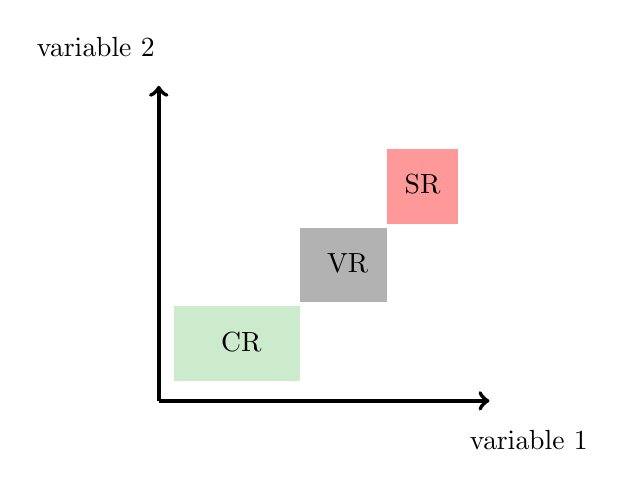
\begin{tikzpicture}
		\draw[line width =1.5pt,->] (0,0) -- (4.2,0);
		\node[](A) at (4.7,-0.5) {variable 1};
		\draw[line width =1.5pt,->] (0,0) -- (0,4.0);
		\node[](B) at (-0.8,4.5) {variable 2};
		\fill[green!60!black!20] (0.2,0.25) rectangle (1.8,1.2);
		\node[](E) at (1.05,0.75) {CR};
		\fill[gray!60] (1.8,1.25) rectangle (2.9,2.2);
%				\fill[gray!60] (1.8,1.25) rectangle (2.9,2.2);
		\node[](L) at (2.4,1.75) {VR};
		\fill[red!40] (2.9,2.25) rectangle (3.8,3.2);
		\node[](M) at (3.35,2.75) {SR};
		\end{tikzpicture}
		\caption{Visualisation of signal, control and validation regions and a typical arrangement in phase space \label{fig:stat:regions}}
\end{figure}



\section{Signal region optimisation}
\label{sec:analysis:sroptimisationSection}
In the following, a description of the optimisation procedure used to define the signal regions is given.
A grid of simulated signal events obtained by varying the masses of \None and \Cone / \Ntwo has been used to perform the signal region optimisation.
The overall signal mass point grid can be seen in Figure \ref{fig:analysis:grid}.
%This includes an extension of the available mass points towards higher \Mntwo masses,  which where not yet available at the optimisation stage of the analysis described below.  This extension is not impacting the sensitivity reach or signal region definition of the analysis.

\subsection{Choice of kinematic variables}
To understand the difference between a potential supersymmetric particle production compared to a \ac{SM} process,  various kinematic variables can be studied.  \\
%This can be properties of the reconstructed particles, such as the transverse momentum ($p_T$),  pseudorapidity ($\eta$) and azimuthal angle $\Phi$,  as well as kinematic variables constructed from these properties.
One of the kinematic variables of interest in a di-tau final state is the \textit{visible mass} of the di-tau system, $m_{vis}(\tau_1,\tau_2)$, constructed using the four-momenta of the two leading tau candidates in the event.  This variable only takes into account the visible components of the hadronic decaying tau, therefore not considering the missing momentum carried by the tau neutrinos.

%In the case of a particle's decay product being invisible to the ATLAS detector,  a part of the momentum will be missing,  shifting the particle's invariant mass calculation.
To account for the invisible decay products,  the missing transverse momentum can be included in an adapted "invisible" mass, the transverse mass $m_T$:

\begin{align}
\label{eq:sr_optimisation:mt} m_T = \sqrt{2p_T^{\ell}E_T^{\text{miss}}(1-\cos(\Delta \phi(\vec{\ell},\vec{p}_T^{\text{miss}}))}
\end{align}

For example,  in the case of a leptonic W-bosons decay, the $m_T$ shows an endpoint at the mass of the W boson. \\
In the case of two hadronically decaying tau leptons,  the sum of the transverse masses $m_{Tsum}$ can be powerful in discriminating \ac{SM} background from signal:

\begin{align}
\label{eq:sr_optimisation:mtsum} m_{Tsum} = m_T(\tau_1)+m_T(\tau_2)
\end{align}

With $m_T(\tau_1)$ denoting the transverse mass as defined in equation \eqref{eq:sr_optimisation:mt} with the lepton as the leading,  highest momentum, hadronic decaying tau lepton. 
The transverse mass concept can be extended to pair produced particles partially decaying into invisible particles, using the definition by Barr, Lester,  Stephens and Summers \cite{mt2original, mt2discussion} of the stransverse mass:

\begin{align}
m_{T2} ( \textbf{p}_T^{\ell_1}, \textbf{p}_T^{\ell_2}, \textbf{p}_T^{\text{miss}}) \equiv  \underset{\textbf{p}_1^\text{miss} + \textbf{p}_2^\text{miss} = \textbf{p}_T^\text{miss}}{\text{min}} \left[ \text{max} \{ m_T(\textbf{p}_T^{\ell_1}, \textbf{p}_1^{\text{miss}}),   m_T(\textbf{p}_T^{\ell_2}, \textbf{p}_2^{\text{miss}}) \} \right]
\end{align}

Here the momentum ($\textbf{p}_T^{\ell_1}, \textbf{p}_T^{\ell_2}$) of the two leptons in the event (for example the visible part of the hadronic tau decay) are combined into a transverse mass with parts of the missing transverse momentum, split into $\textbf{p}_1^\text{miss}$ and $\textbf{p}_2^\text{miss}$.  
This variable shows an endpoint at the mass of the pair-produced particle,  leading to a usually lower end-point of the distribution for \ac{SM} background processes in comparison to the \ac{SUSY} model considered. The mass of the invisible particles is assumed to be zero.

If an event includes more than two leptons (with a maximum number of leptons $n_\ell$),  it can be useful to perform a maximisation over the $m_{T2}$ values resulting from all possible lepton pairs:

\begin{align}
m_{T2}^\text{max} = \max_{\substack{i = 1,...,n_\ell \\ j = 2,..., n_\ell \\ i \neq j}} \left[ m_{T2}(\textbf{p}_T^{\ell_i}, \textbf{p}_T^ {\ell_j},\textbf{p}_T^{\text{miss}}) \right] \label{eq:sr_optimisation:mt2max}
\end{align}

\FloatBarrier
\subsection{SR optimisation procedure}
As starting point of the optimisation,  the kinematic variables described in the previous section are studied for \ac{SM} background events and signal events. In the following plots, all \ac{SM} background distributions shown are obtained from Monte Carlo.
In Figure \ref{fig:app:LMpreselections}, some kinematic variables are shown after the selection with an asymmetric di-tau trigger selection as well as a b-jet veto and light lepton veto.  %These preselections are used to gauge the discriminating power of a set of kinematic variables for varying signal mass points.
A selection of signal points is used to gauge the effectiveness of the variables to isolate a signal.
In Figure \ref{fig:analysis:opt:mt2max},  $m_{T2}^\text{max}$,  as defined in \eqref{eq:sr_optimisation:mt2max} can be compared with Figure \ref{fig:analysis:opt:mt2},  showing $m_{T2}$. The maximisation over all tau pairs in the event leads to a slight improvement in sensitivity compared to $m_{T2}$ calculated using the two leading tau candidates.  In the lower panels of Figure \ref{fig:app:LMpreselections},  a simplified sensitivity measure $Z_n$ \cite{zndefinition} including a 30\% flat systematic uncertainty is used to gauge the sensitivity of each variable to the signal model.  A $Z_n$ implementation of the RooStats \cite{RooStats} package within the ROOT \cite{Root} software framework is used.  This sensitivity measure is used to estimate the signal to background separation power as fully estimated with hypothesis testing as described in section \ref{sec:analysis:stats}.
As can be seen in Figures \ref{fig:analysis:opt:mttau1} and Fig.  \ref{fig:analysis:opt:mttau2} in comparison to the sum of both $m_T$ shown in Figure \ref{fig:analysis:opt:summt},  summing the transverse mass of the two leading taus offers a slightly higher discriminating power than the single transverse masses.
%/mnt/lustre/projects/epp/general/atlas/dk352/C1N2_tau/plotting_kinematics/19v02plotting/April20/210420_optimising

\begin{figure}[htpb]
\centering
\subfloat[$m_{T2}^\text{max}$ \label{fig:analysis:opt:mt2max} ]{\includegraphics[width=0.49\textwidth]{figures/SignalOp_Thesis_260722_AG_noATLAS/asymbasicLLV_mt2maxSROpt.pdf}}
\subfloat[$m_{T2}$ \label{fig:analysis:opt:mt2}]{\includegraphics[width=0.49\textwidth]{figures/SignalOp_Thesis_260722_AG_noATLAS/asymbasicLLV_mt2SROpt.pdf}}\\
\subfloat[$m_T(\tau_1,E_T^\text{miss})$ \label{fig:analysis:opt:mttau1}]{\includegraphics[width=0.49\textwidth]{figures/SignalOp_Thesis_260722_AG_noATLAS/asymbasicLLV_Mt_Tau1metSROpt.pdf}}
\subfloat[$m_T(\tau_2,E_T^\text{miss})$ \label{fig:analysis:opt:mttau2}]{\includegraphics[width=0.49\textwidth]{figures/SignalOp_Thesis_260722_AG_noATLAS/asymbasicLLV_Mt_Tau2metSROpt.pdf}}\\
\subfloat[$m_{Tsum}$ \label{fig:analysis:opt:summt}]{\includegraphics[width=0.49\textwidth]{figures/SignalOp_Thesis_260722_AG_noATLAS/asymbasicLLV_SumMtTauSROpt.pdf}}
\subfloat[$m_{vis}(\tau_1,\tau_2)$ \label{fig:analysis:opt:mvis}]{\includegraphics[width=0.49\textwidth]{figures/SignalOp_Thesis_260722_AG_noATLAS/asymbasicLLV_mvisTauTauSROpt.pdf}}\\
\subfloat[$E_T^\text{miss}$ \label{fig:analysis:opt:met}]{\includegraphics[width=0.49\textwidth]{figures/SignalOp_Thesis_260722_AG_noATLAS/asymbasicLLV_metSROpt.pdf}}
%\subfloat[$meff$]{\includegraphics[width=0.45\textwidth]{figures/C1N2SS/SROptAppendix/asym_basicLLV_meff_mc16_a_e_d_.pdf}} \\
\subfloat[$\Delta\phi(\tau_1,\tau_2)$ \label{fig:analysis:opt:deltaphi}]{\includegraphics[width=0.49\textwidth]{figures/SignalOp_Thesis_260722_AG_noATLAS/asymbasicLLV_deltaPhiTauTauSROpt.pdf}}
%\subfloat[$\Delta\phi(\tau_1,E_T^\text{miss})$]{\includegraphics[width=0.45\textwidth]{figures/C1N2SS/SROptAppendix/asym_basicLLV_deltaPhiTau1Met_mc16_a_e_d_.pdf}}
\caption{Kinematic variable distributions for SS scenario after a loose preselection. Error bands include statistical uncertainties only.  The lower panel shows the significance $Z_n$ including a 30 \% systematic uncertainty assumption. 
\label{fig:app:LMpreselections}}
\end{figure}

%210420_improveSign

In case of a low m(\Cone,\Ntwo) (low mass scenario, SR-C1N2SS-LM),  a cut of $E_T^\text{miss} < 150 \text{ GeV}$ is introduced.  The case of high \Cone, \Ntwo mass (SR-C1N2SS-HM) is defined by $E_T^\text{miss}>~150 \text{ GeV}$. The effect of multiple cuts (not applied consecutively) on the overall sensitivity is given in Figure~\ref{fig:app:LMgridstudies}.



\begin{figure}[h]
\centering
\subfloat[$m_{T2}^\text{max} > 20 \text{ GeV} $]{\includegraphics[width=0.49\textwidth]{figures/C1N2SS/SROptAppendix_Improved/SignificancesTrueonlymt2_20.pdf}}
\subfloat[$m_{T2}^\text{max} > 50 \text{ GeV} $]{\includegraphics[width=0.49\textwidth]{figures/C1N2SS/SROptAppendix_Improved/SignificancesTrueonlymt2_50.pdf}} \\
\subfloat[$m_{Tsum} > 150 \text{ GeV}$]{\includegraphics[width=0.49\textwidth]{figures/C1N2SS/SROptAppendix_Improved/SignificancesTrueonlySumMt_150.pdf}}
\subfloat[$m_{Tsum} > 200 \text{ GeV}$]{\includegraphics[width=0.49\textwidth]{figures/C1N2SS/SROptAppendix_Improved/SignificancesTrueonlySumMt_200.pdf}}\\
\caption{ Significance estimation including a $30 \%$ flat systematic uncertainty.\label{fig:app:LMgridstudies}}
\end{figure}

An $m_{Tsum} > 200 \text{ GeV}$ selection was chosen because it gives a higher sensitivity toward the diagonal of the (\Cone/\Ntwo, \None) mass plane.
The additional requirement $\Delta\phi(\tau_1,\tau_2) > 1.5$ is included in the signal region definition,  to reduce the signal contamination when estimating the multi-jet background (see section \ref{sec:bkgestimation:ABCD}.
The optimisation for the high mass case followed a very similar approach, leading to the two orthogonal signal regions defined in Table~\ref{tab:SRdef}.
%This selection and an inversion of the transverse mass sum requirement offered the basis of the ABCD method,  allowing for a multi-jet estimation.  This is in detail described in section \ref{sec:bkgestimation:ABCD}.
%A preliminary estimation of the multi-jet background lead to the introduction of a $\Delta\phi(\tau_1,\tau_2)+\Delta\phi(\tau_1, E_T^\text{miss})>2.5$ cut to reduce the signal contamination within the ABCD regions.


%With a multi-jet background estimate included, multiple further cuts on kinematic variables have been tested according to their performance over the grid, with a particular focus on the sensitivitiy towards the kinematic diagonal (\Mnone close to \Mntwo). These include:
%\begin{itemize}
%\item $m_T(\tau_1)+m_T(\tau_2)$ > [240, 260, 280, 300,400,500]
%\item $m_{vis}(\tau_1,\tau_2) > 130$, $m_{vis}(\tau_1,\tau_2) > 400$, $m_{vis}(\tau_1,\tau_2) \in [130,400]$
%\item $E_T^\text{miss}$ > [50,60,70,80]
%\item $m_{T2}^\text{max}$ > [10,20,30,40,50,60,70,80]
%\item Number of signal jets < [2,3]
%\end{itemize}

%Multiple different combinations of these cuts have been taken into account and their effect considered singular as well as in combination. These iterative studies led to the definitions given in section \ref{sec:SR:SS}.

 %The sum of the leading taus transverse mass ($m_T(\tau_1)+m_T(\tau_2)$) was used to define ABCD regions and with that a signal region optimisation phase space, using a $m_T(\tau_1)+m_T(\tau_2) > 300 \text{GeV}$ requirement.

%%%%%%%%%%%%%%%%%%%%%%%%%%%%%%%%%%%%%%%%%%%%%%%%%%%%%%%%%%%%%%%%%%%%%%%%%%%%%%%%%%%


\begin{table}[htpb!]
\centering
\begin{tabular}{c|c} \hline
SR-C1N2SS-LM & SR-C1N2SS-HM \\ \hline \hline
\multicolumn{2}{c}{$>=$ 2 medium taus (SS) } \\
\multicolumn{2}{c}{$b$-jet veto} \\
$\Delta\Phi(\tau_1,\tau_2)  > 1.5 $&-\\
${N}_{jets} <$3 & - \\ \hline
$m_{Tsum}  > 200 \text{ GeV} $ & $m_{Tsum} > 450 \text{ GeV}$\\
\multicolumn{2}{c}{$ m_{T2}^{\text{max}} > 80 \text{ GeV}$  } \\\hline %\vspace{0.5cm}\\ \hline %\vspace{1cm}
 asymmetric di-tau trigger  & di-tau+\met trigger \\
$\met <$ 150 GeV    & $\met >$ 150 GeV          \\
\multicolumn{2}{c}{$\tau_{1}$ and $\tau_{2}$ $p_\text{T}$ requirements described in Table
  \ref{tab:analysis:trigger} in Section \ref{sec:analysis:eventselection}}\\
\hline
\end{tabular}
\caption{Summary of selection requirements for the signal regions.
\label{tab:SRdef} }
\end{table}

An overview of the event yields in both signal regions is shown in table \ref{tab:SS:SRyields}. All backgrounds apart from the Multi-jet background are taken from MC simulation with only statistical uncertainties included below.  The Multijet estimation is performed using a data-driven method,  discussed in detail in section \ref{sec:bkgestimation:ABCD}.

\begin{table}
\centering
% Preview source code for paragraph 0

\begin{tabular}{c|c|c}
\hline
SM-process & SR-C1N2SS-LM & SR-C1N2SS-HM\tabularnewline
\hline
\hline
%\hline
Top & $0.01\pm0.01$ & $0.84\pm0.36$\tabularnewline
%\hline
Multi-boson & $0.47\pm0.11$ & $0.81\pm0.21$\tabularnewline
%\hline
Multi-jet & $0.94\pm0.27$ & $ -0.086 \pm 0.31$\tabularnewline
%\hline
$W$+jets & $0.32\pm0.32$ & $0.10\pm0.10$\tabularnewline
%\hline
$Z$+jets & $0.20\pm0.20$ & $0.59\pm0.56$\tabularnewline
%\hline
Higgs & $0.00\pm0.00$ & $0.02\pm0.00$\tabularnewline
\hline
%\hline
SM total & $1.95 \pm 0.48$ & $2.35\pm0.80$\tabularnewline
%\hline
\hline
%Ref. point (325, 175) & $18.20\pm3.00$ & $2.91\pm0.51$\tabularnewline
Ref. point (325, 175) & $ 7.80 \pm 1.27 $& $ 2.26 \pm 0.71 $\tabularnewline
%\hline
%Ref. point (500, 300)  & $5.25\pm0.75$ & $4.68\pm10.78$\tabularnewline
Ref. point (500, 300)  & $ 3.78 \pm 0.65 $& $ 5.62 \pm 0.88 $\tabularnewline
%\hline
%Ref. point (900, 300) & $0.71\pm0.07$ & $6.37\pm0.21$\tabularnewline
Ref. point (900, 300) &  $ 0.84 \pm 0.07 $ & $ 6.23 \pm 0.21 $\tabularnewline
\hline
\end{tabular}
\caption{Number of events in the signal regions for SM backgrounds, including statistical
  uncertainties.  The SM MC backgrounds are normalised to 139~\ifb. The multi-jet contribution is estimated
  from data with a simplified ABCD method described in Section
  \ref{sec:bkgestimation:ABCD}. Only statistical uncertainty are considered for MC
  estimated processes and multi-jet.
%The proper results are showed in Table~\ref{ysr0} in Section \ref{sec:results-bkgfit}.
\label{tab:SS:SRyields}}
\end{table}

%%%%%%%%%%%%%%%%%%%%%%%%%%%%%%%%%%%%%%%%%%%%%%%%%%%%%%%%%%%%%%%%%%%%%%%%%%%%%%%%%%%
%%%%    N-1 plots
%%%%%%%%%%%%%%%%%%%%%%%%%%%%%%%%%%%%%%%%%%%%%%%%%%%%%%%%%%%%%%%%%%%%%%%%%%%%%%%%%%%

Kinematic distributions in the signal regions, with requirements on the shown variable removed ("N-1 distributions"), can be seen in figure \ref{fig:SS:SRlowmass} for SR-C1N2SS-LM,  and figure \ref{fig:SS:SRhighmass} for SR-C1N2SS-HM,  already including the multi-jet estimation as well as systematic uncertainties discussed in section \ref{sec:analysis:bkgestimation} and \ref{sec:analysis:systematics}, respectively. 

\begin{figure}[!htpb]
\centering
  \subfloat[$\Delta\Phi(\tau_1,\tau_2)$]{\includegraphics[width=0.49\textwidth]{figures/UpdatedThesisFigures_noATLAS/LowMass/DeltaPhi_N1_improved.pdf}}
  \subfloat[${N}_{jets} $]{\includegraphics[width=0.49\textwidth]{figures/UpdatedThesisFigures_noATLAS/LowMass/SigJets_N1_improved.pdf}}\\
  \subfloat[$ m_{T2}^{\text{max}} $]{\includegraphics[width=0.49\textwidth]{figures/UpdatedThesisFigures_noATLAS/LowMass/Mt2_N1_improved.pdf}}
  \caption{``N-1'' distributions of relevant kinematic variables after SR-C1N2SS-LM requirements, except the one on the
shown variable, have been applied.
The stacked histograms show the expected SM backgrounds estimated from \ac{MC}, normalised to 139~\ifb as well as Multi-jet expectation as described in section \ref{sec:bkgestimation:ABCD}.
\label{fig:SS:SRlowmass}Statistical uncertainties and systematic uncertainties as discussed in section \ref{sec:analysis:systematics} are included in the error band. }
\end{figure}

\begin{figure}[!htpb]
\centering
\subfloat[$m_{Tsum}$]{\includegraphics[width=0.49\textwidth]{figures/UpdatedThesisFigures_noATLAS/HighMass/SumMt_N1_improved.pdf}}
\subfloat[$ m_{T2}^{\text{max}} $]{\includegraphics[width=0.49\textwidth]{figures/UpdatedThesisFigures_noATLAS/HighMass/Mt2_N1_improved.pdf}}
  \caption{``N-1'' distributions of relevant kinematic variables after SR-C1N2SS-HM requirements, except the one on the
shown variable, have been applied. The stacked histograms show the expected \ac{SM} backgrounds estimated from \ac{MC}, normalised to 139 ~\ifb as well as Multi-jet expectation as described in section \ref{sec:bkgestimation:ABCD}. Statistical and systematic uncertainties as discussed in \ref{sec:analysis:systematics} are included in the error band. 
\label{fig:SS:SRhighmass} }
\end{figure}

Further kinematic distribution in both signal regions can be seen in \ref{fig:SS:SRlowDistr} and \ref{fig:SS:SRhighDistr}, respectively. This clearly shows that no further requirements on other kinematic variables are able to gain in sensitivity,  at least not while allowing for sufficient remaining statistics in the \ac{SM} background simulations.

\begin{figure}[!htpb]
\centering
\subfloat[]{\includegraphics[width=0.49\textwidth]{figures/UpdatedThesisFigures_noATLAS/LowMass/asymSRD_wDPhiOnly_TRIALsummt200_mvis_nomvisup_MT280_deltaphi_signaljets2_noLLV_nomvis_deltaPhiTau1MetSRL.pdf}}
\subfloat[]{\includegraphics[width=0.49\textwidth]{figures/UpdatedThesisFigures_noATLAS/LowMass/asymSRD_wDPhiOnly_TRIALsummt200_mvis_nomvisup_MT280_deltaphi_signaljets2_noLLV_nomvis_deltaR_etaSRL.pdf}}\\
\subfloat[]{\includegraphics[width=0.49\textwidth]{figures/UpdatedThesisFigures_noATLAS/LowMass/asymSRD_wDPhiOnly_TRIALsummt200_mvis_nomvisup_MT280_deltaphi_signaljets2_noLLV_nomvis_metSRL.pdf}}
\subfloat[]{\includegraphics[width=0.49\textwidth]{figures/UpdatedThesisFigures_noATLAS/LowMass/asymSRD_wDPhiOnly_TRIALsummt200_mvis_nomvisup_MT280_deltaphi_signaljets2_noLLV_nomvis_tau1PtSRL.pdf}}\\
\subfloat[]{\includegraphics[width=0.49\textwidth]{figures/UpdatedThesisFigures_noATLAS/LowMass/asymSRD_wDPhiOnly_TRIALsummt200_mvis_nomvisup_MT280_deltaphi_signaljets2_noLLV_nomvis_tau2PtSRH.pdf}}
\subfloat[]{\includegraphics[width=0.49\textwidth]{figures/UpdatedThesisFigures_noATLAS/LowMass/asymSRD_wDPhiOnly_TRIALsummt200_mvis_nomvisup_MT280_deltaphi_signaljets2_noLLV_nomvis_mvisTauTauSRL.pdf}}
  \caption{Remaining kinematic distributions in SR-C1N2SS-LM, for all variables not used in the signal region definition.  The error band includes statistical and systematic uncertainties. The lower panel shows the significance $Z_n$ including a 30 \% systematic uncertainty assumption. 
\label{fig:SS:SRlowDistr}}.
\end{figure}

\begin{figure}[!htpb]
\centering
  \subfloat[]{\includegraphics[width=0.49\textwidth]{figures//UpdatedThesisFigures_noATLAS/HighMass/ditauMETSRSummthighmt2_deltaEtaTauTau.pdf} }
  \subfloat[]{\includegraphics[width=0.49\textwidth]{figures//UpdatedThesisFigures_noATLAS/HighMass/ditauMETSRSummthighmt2_deltaPhiTau1MetSRL.pdf} }\\
  \subfloat[]{\includegraphics[width=0.49\textwidth]{figures//UpdatedThesisFigures_noATLAS/HighMass/ditauMETSRSummthighmt2_deltaPhiTauTauSRH.pdf} }
     \subfloat[]{\includegraphics[width=0.49\textwidth]{figures//UpdatedThesisFigures_noATLAS/HighMass/ditauMETSRSummthighmt2_deltaR_etaSRL.pdf} }\\
  \subfloat[]{\includegraphics[width=0.49\textwidth]{figures/UpdatedThesisFigures_noATLAS/HighMass/ditauMETSRSummthighmt2_metSRH.pdf} }
  \subfloat[]{\includegraphics[width=0.49\textwidth]{figures/UpdatedThesisFigures_noATLAS/HighMass/ditauMETSRSummthighmt2_mvisTauTauSRH.pdf} }
  \caption{Remaining kinematic distributions in SR-C1N2SS-HM, for all variables not used in the signal region definition. The error band includes statistical and systematic uncertainties. The lower panel shows the significance $Z_n$ including a 30 \% systematic uncertainty assumption. 
\label{fig:SS:SRhighDistr}}
\end{figure}


%%%%%%%%%%%%%%%%%%%%%%%%%%%%%%%%%%%%%%%%%%%%%%%%%%%%%%%%%%%%%%%%%%%%%%%%%%%%%%%%%%%
%%%% sensitivity
%%%%%%%%%%%%%%%%%%%%%%%%%%%%%%%%%%%%%%%%%%%%%%%%%%%%%%%%%%%%%%%%%%%%%%%%%%%%%%%%%%%
 The estimated sensitivity of both signal regions, using the significance measure $Z_n$ is shown in figure \ref{fig:SS:SRsign}. This is a first estimate of the sensitivity of these regions to the gaugino pair production under investigation.

\begin{figure}[!htpb]
\centering
  \subfloat[SR-C1N2SS-LM]{\includegraphics[width=0.49\textwidth]{figures/C1N2SS/SRdefs/LowMass/SRLowMassSign_improved.pdf}}
  \subfloat[SR-C1N2SS-HM]{\includegraphics[width=0.49\textwidth]{figures/C1N2SS/SRdefs/HighMass/SRHighMassSign_improved.pdf}}
  \caption{Significance distribution for the (a) SR-C1N2SS-LM, (b)
  SR-C1N2SS-HM for 139~\ifb. The statistical uncertainty
 and 30\% systematic uncertainty on SM backgrounds are included in the $\text{Z}_{\text{N}}$
calculation. 
\label{fig:SS:SRsign}}
\end{figure}

\label{sec:analysis:sroptimisation}

%In the following, a description of the optimisation procedure used to define the signal regions is given.
A grid of simulated signal events obtained by varying the masses of \None and \Cone / \Ntwo has been used to perform the signal region optimisation.
The overall signal mass point grid can be seen in Figure \ref{fig:analysis:grid}.
%This includes an extension of the available mass points towards higher \Mntwo masses,  which where not yet available at the optimisation stage of the analysis described below.  This extension is not impacting the sensitivity reach or signal region definition of the analysis.

\subsection{Choice of kinematic variables}
To understand the difference between a potential supersymmetric particle production compared to a \ac{SM} process,  various kinematic variables can be studied.  \\
%This can be properties of the reconstructed particles, such as the transverse momentum ($p_T$),  pseudorapidity ($\eta$) and azimuthal angle $\Phi$,  as well as kinematic variables constructed from these properties.
One of the kinematic variables of interest in a di-tau final state is the \textit{visible mass} of the di-tau system, $m_{vis}(\tau_1,\tau_2)$, constructed using the four-momenta of the two leading tau candidates in the event.  This variable only takes into account the visible components of the hadronic decaying tau, therefore not considering the missing momentum carried by the tau neutrinos.

%In the case of a particle's decay product being invisible to the ATLAS detector,  a part of the momentum will be missing,  shifting the particle's invariant mass calculation.
To account for the invisible decay products,  the missing transverse momentum can be included in an adapted "invisible" mass, the transverse mass $m_T$:

\begin{align}
\label{eq:sr_optimisation:mt} m_T = \sqrt{2p_T^{\ell}E_T^{\text{miss}}(1-\cos(\Delta \phi(\vec{\ell},\vec{p}_T^{\text{miss}}))}
\end{align}

For example,  in the case of a leptonic W-bosons decay, the $m_T$ shows an endpoint at the mass of the W boson. \\
In the case of two hadronically decaying tau leptons,  the sum of the transverse masses $m_{Tsum}$ can be powerful in discriminating \ac{SM} background from signal:

\begin{align}
\label{eq:sr_optimisation:mtsum} m_{Tsum} = m_T(\tau_1)+m_T(\tau_2)
\end{align}

With $m_T(\tau_1)$ denoting the transverse mass as defined in equation \eqref{eq:sr_optimisation:mt} with the lepton as the leading,  highest momentum, hadronic decaying tau lepton. 
The transverse mass concept can be extended to pair produced particles partially decaying into invisible particles, using the definition by Barr, Lester,  Stephens and Summers \cite{mt2original, mt2discussion} of the stransverse mass:

\begin{align}
m_{T2} ( \textbf{p}_T^{\ell_1}, \textbf{p}_T^{\ell_2}, \textbf{p}_T^{\text{miss}}) \equiv  \underset{\textbf{p}_1^\text{miss} + \textbf{p}_2^\text{miss} = \textbf{p}_T^\text{miss}}{\text{min}} \left[ \text{max} \{ m_T(\textbf{p}_T^{\ell_1}, \textbf{p}_1^{\text{miss}}),   m_T(\textbf{p}_T^{\ell_2}, \textbf{p}_2^{\text{miss}}) \} \right]
\end{align}

Here the momentum ($\textbf{p}_T^{\ell_1}, \textbf{p}_T^{\ell_2}$) of the two leptons in the event (for example the visible part of the hadronic tau decay) are combined into a transverse mass with parts of the missing transverse momentum, split into $\textbf{p}_1^\text{miss}$ and $\textbf{p}_2^\text{miss}$.  
This variable shows an endpoint at the mass of the pair-produced particle,  leading to a usually lower end-point of the distribution for \ac{SM} background processes in comparison to the \ac{SUSY} model considered. The mass of the invisible particles is assumed to be zero.

If an event includes more than two leptons (with a maximum number of leptons $n_\ell$),  it can be useful to perform a maximisation over the $m_{T2}$ values resulting from all possible lepton pairs:

\begin{align}
m_{T2}^\text{max} = \max_{\substack{i = 1,...,n_\ell \\ j = 2,..., n_\ell \\ i \neq j}} \left[ m_{T2}(\textbf{p}_T^{\ell_i}, \textbf{p}_T^ {\ell_j},\textbf{p}_T^{\text{miss}}) \right] \label{eq:sr_optimisation:mt2max}
\end{align}

\FloatBarrier
\subsection{SR optimisation procedure}
As starting point of the optimisation,  the kinematic variables described in the previous section are studied for \ac{SM} background events and signal events. In the following plots, all \ac{SM} background distributions shown are obtained from Monte Carlo.
In Figure \ref{fig:app:LMpreselections}, some kinematic variables are shown after the selection with an asymmetric di-tau trigger selection as well as a b-jet veto and light lepton veto.  %These preselections are used to gauge the discriminating power of a set of kinematic variables for varying signal mass points.
A selection of signal points is used to gauge the effectiveness of the variables to isolate a signal.
In Figure \ref{fig:analysis:opt:mt2max},  $m_{T2}^\text{max}$,  as defined in \eqref{eq:sr_optimisation:mt2max} can be compared with Figure \ref{fig:analysis:opt:mt2},  showing $m_{T2}$. The maximisation over all tau pairs in the event leads to a slight improvement in sensitivity compared to $m_{T2}$ calculated using the two leading tau candidates.  In the lower panels of Figure \ref{fig:app:LMpreselections},  a simplified sensitivity measure $Z_n$ \cite{zndefinition} including a 30\% flat systematic uncertainty is used to gauge the sensitivity of each variable to the signal model.  A $Z_n$ implementation of the RooStats \cite{RooStats} package within the ROOT \cite{Root} software framework is used.  This sensitivity measure is used to estimate the signal to background separation power as fully estimated with hypothesis testing as described in section \ref{sec:analysis:stats}.
As can be seen in Figures \ref{fig:analysis:opt:mttau1} and Fig.  \ref{fig:analysis:opt:mttau2} in comparison to the sum of both $m_T$ shown in Figure \ref{fig:analysis:opt:summt},  summing the transverse mass of the two leading taus offers a slightly higher discriminating power than the single transverse masses.
%/mnt/lustre/projects/epp/general/atlas/dk352/C1N2_tau/plotting_kinematics/19v02plotting/April20/210420_optimising

\begin{figure}[htpb]
\centering
\subfloat[$m_{T2}^\text{max}$ \label{fig:analysis:opt:mt2max} ]{\includegraphics[width=0.49\textwidth]{figures/SignalOp_Thesis_260722_AG_noATLAS/asymbasicLLV_mt2maxSROpt.pdf}}
\subfloat[$m_{T2}$ \label{fig:analysis:opt:mt2}]{\includegraphics[width=0.49\textwidth]{figures/SignalOp_Thesis_260722_AG_noATLAS/asymbasicLLV_mt2SROpt.pdf}}\\
\subfloat[$m_T(\tau_1,E_T^\text{miss})$ \label{fig:analysis:opt:mttau1}]{\includegraphics[width=0.49\textwidth]{figures/SignalOp_Thesis_260722_AG_noATLAS/asymbasicLLV_Mt_Tau1metSROpt.pdf}}
\subfloat[$m_T(\tau_2,E_T^\text{miss})$ \label{fig:analysis:opt:mttau2}]{\includegraphics[width=0.49\textwidth]{figures/SignalOp_Thesis_260722_AG_noATLAS/asymbasicLLV_Mt_Tau2metSROpt.pdf}}\\
\subfloat[$m_{Tsum}$ \label{fig:analysis:opt:summt}]{\includegraphics[width=0.49\textwidth]{figures/SignalOp_Thesis_260722_AG_noATLAS/asymbasicLLV_SumMtTauSROpt.pdf}}
\subfloat[$m_{vis}(\tau_1,\tau_2)$ \label{fig:analysis:opt:mvis}]{\includegraphics[width=0.49\textwidth]{figures/SignalOp_Thesis_260722_AG_noATLAS/asymbasicLLV_mvisTauTauSROpt.pdf}}\\
\subfloat[$E_T^\text{miss}$ \label{fig:analysis:opt:met}]{\includegraphics[width=0.49\textwidth]{figures/SignalOp_Thesis_260722_AG_noATLAS/asymbasicLLV_metSROpt.pdf}}
%\subfloat[$meff$]{\includegraphics[width=0.45\textwidth]{figures/C1N2SS/SROptAppendix/asym_basicLLV_meff_mc16_a_e_d_.pdf}} \\
\subfloat[$\Delta\phi(\tau_1,\tau_2)$ \label{fig:analysis:opt:deltaphi}]{\includegraphics[width=0.49\textwidth]{figures/SignalOp_Thesis_260722_AG_noATLAS/asymbasicLLV_deltaPhiTauTauSROpt.pdf}}
%\subfloat[$\Delta\phi(\tau_1,E_T^\text{miss})$]{\includegraphics[width=0.45\textwidth]{figures/C1N2SS/SROptAppendix/asym_basicLLV_deltaPhiTau1Met_mc16_a_e_d_.pdf}}
\caption{Kinematic variable distributions for SS scenario after a loose preselection. Error bands include statistical uncertainties only.  The lower panel shows the significance $Z_n$ including a 30 \% systematic uncertainty assumption. 
\label{fig:app:LMpreselections}}
\end{figure}

%210420_improveSign

In case of a low m(\Cone,\Ntwo) (low mass scenario, SR-C1N2SS-LM),  a cut of $E_T^\text{miss} < 150 \text{ GeV}$ is introduced.  The case of high \Cone, \Ntwo mass (SR-C1N2SS-HM) is defined by $E_T^\text{miss}>~150 \text{ GeV}$. The effect of multiple cuts (not applied consecutively) on the overall sensitivity is given in Figure~\ref{fig:app:LMgridstudies}.



\begin{figure}[h]
\centering
\subfloat[$m_{T2}^\text{max} > 20 \text{ GeV} $]{\includegraphics[width=0.49\textwidth]{figures/C1N2SS/SROptAppendix_Improved/SignificancesTrueonlymt2_20.pdf}}
\subfloat[$m_{T2}^\text{max} > 50 \text{ GeV} $]{\includegraphics[width=0.49\textwidth]{figures/C1N2SS/SROptAppendix_Improved/SignificancesTrueonlymt2_50.pdf}} \\
\subfloat[$m_{Tsum} > 150 \text{ GeV}$]{\includegraphics[width=0.49\textwidth]{figures/C1N2SS/SROptAppendix_Improved/SignificancesTrueonlySumMt_150.pdf}}
\subfloat[$m_{Tsum} > 200 \text{ GeV}$]{\includegraphics[width=0.49\textwidth]{figures/C1N2SS/SROptAppendix_Improved/SignificancesTrueonlySumMt_200.pdf}}\\
\caption{ Significance estimation including a $30 \%$ flat systematic uncertainty.\label{fig:app:LMgridstudies}}
\end{figure}

An $m_{Tsum} > 200 \text{ GeV}$ selection was chosen because it gives a higher sensitivity toward the diagonal of the (\Cone/\Ntwo, \None) mass plane.
The additional requirement $\Delta\phi(\tau_1,\tau_2) > 1.5$ is included in the signal region definition,  to reduce the signal contamination when estimating the multi-jet background (see section \ref{sec:bkgestimation:ABCD}.
The optimisation for the high mass case followed a very similar approach, leading to the two orthogonal signal regions defined in Table~\ref{tab:SRdef}.
%This selection and an inversion of the transverse mass sum requirement offered the basis of the ABCD method,  allowing for a multi-jet estimation.  This is in detail described in section \ref{sec:bkgestimation:ABCD}.
%A preliminary estimation of the multi-jet background lead to the introduction of a $\Delta\phi(\tau_1,\tau_2)+\Delta\phi(\tau_1, E_T^\text{miss})>2.5$ cut to reduce the signal contamination within the ABCD regions.


%With a multi-jet background estimate included, multiple further cuts on kinematic variables have been tested according to their performance over the grid, with a particular focus on the sensitivitiy towards the kinematic diagonal (\Mnone close to \Mntwo). These include:
%\begin{itemize}
%\item $m_T(\tau_1)+m_T(\tau_2)$ > [240, 260, 280, 300,400,500]
%\item $m_{vis}(\tau_1,\tau_2) > 130$, $m_{vis}(\tau_1,\tau_2) > 400$, $m_{vis}(\tau_1,\tau_2) \in [130,400]$
%\item $E_T^\text{miss}$ > [50,60,70,80]
%\item $m_{T2}^\text{max}$ > [10,20,30,40,50,60,70,80]
%\item Number of signal jets < [2,3]
%\end{itemize}

%Multiple different combinations of these cuts have been taken into account and their effect considered singular as well as in combination. These iterative studies led to the definitions given in section \ref{sec:SR:SS}.

 %The sum of the leading taus transverse mass ($m_T(\tau_1)+m_T(\tau_2)$) was used to define ABCD regions and with that a signal region optimisation phase space, using a $m_T(\tau_1)+m_T(\tau_2) > 300 \text{GeV}$ requirement.

%%%%%%%%%%%%%%%%%%%%%%%%%%%%%%%%%%%%%%%%%%%%%%%%%%%%%%%%%%%%%%%%%%%%%%%%%%%%%%%%%%%


\begin{table}[htpb!]
\centering
\begin{tabular}{c|c} \hline
SR-C1N2SS-LM & SR-C1N2SS-HM \\ \hline \hline
\multicolumn{2}{c}{$>=$ 2 medium taus (SS) } \\
\multicolumn{2}{c}{$b$-jet veto} \\
$\Delta\Phi(\tau_1,\tau_2)  > 1.5 $&-\\
${N}_{jets} <$3 & - \\ \hline
$m_{Tsum}  > 200 \text{ GeV} $ & $m_{Tsum} > 450 \text{ GeV}$\\
\multicolumn{2}{c}{$ m_{T2}^{\text{max}} > 80 \text{ GeV}$  } \\\hline %\vspace{0.5cm}\\ \hline %\vspace{1cm}
 asymmetric di-tau trigger  & di-tau+\met trigger \\
$\met <$ 150 GeV    & $\met >$ 150 GeV          \\
\multicolumn{2}{c}{$\tau_{1}$ and $\tau_{2}$ $p_\text{T}$ requirements described in Table
  \ref{tab:analysis:trigger} in Section \ref{sec:analysis:eventselection}}\\
\hline
\end{tabular}
\caption{Summary of selection requirements for the signal regions.
\label{tab:SRdef} }
\end{table}

An overview of the event yields in both signal regions is shown in table \ref{tab:SS:SRyields}. All backgrounds apart from the Multi-jet background are taken from MC simulation with only statistical uncertainties included below.  The Multijet estimation is performed using a data-driven method,  discussed in detail in section \ref{sec:bkgestimation:ABCD}.

\begin{table}
\centering
% Preview source code for paragraph 0

\begin{tabular}{c|c|c}
\hline
SM-process & SR-C1N2SS-LM & SR-C1N2SS-HM\tabularnewline
\hline
\hline
%\hline
Top & $0.01\pm0.01$ & $0.84\pm0.36$\tabularnewline
%\hline
Multi-boson & $0.47\pm0.11$ & $0.81\pm0.21$\tabularnewline
%\hline
Multi-jet & $0.94\pm0.27$ & $ -0.086 \pm 0.31$\tabularnewline
%\hline
$W$+jets & $0.32\pm0.32$ & $0.10\pm0.10$\tabularnewline
%\hline
$Z$+jets & $0.20\pm0.20$ & $0.59\pm0.56$\tabularnewline
%\hline
Higgs & $0.00\pm0.00$ & $0.02\pm0.00$\tabularnewline
\hline
%\hline
SM total & $1.95 \pm 0.48$ & $2.35\pm0.80$\tabularnewline
%\hline
\hline
%Ref. point (325, 175) & $18.20\pm3.00$ & $2.91\pm0.51$\tabularnewline
Ref. point (325, 175) & $ 7.80 \pm 1.27 $& $ 2.26 \pm 0.71 $\tabularnewline
%\hline
%Ref. point (500, 300)  & $5.25\pm0.75$ & $4.68\pm10.78$\tabularnewline
Ref. point (500, 300)  & $ 3.78 \pm 0.65 $& $ 5.62 \pm 0.88 $\tabularnewline
%\hline
%Ref. point (900, 300) & $0.71\pm0.07$ & $6.37\pm0.21$\tabularnewline
Ref. point (900, 300) &  $ 0.84 \pm 0.07 $ & $ 6.23 \pm 0.21 $\tabularnewline
\hline
\end{tabular}
\caption{Number of events in the signal regions for SM backgrounds, including statistical
  uncertainties.  The SM MC backgrounds are normalised to 139~\ifb. The multi-jet contribution is estimated
  from data with a simplified ABCD method described in Section
  \ref{sec:bkgestimation:ABCD}. Only statistical uncertainty are considered for MC
  estimated processes and multi-jet.
%The proper results are showed in Table~\ref{ysr0} in Section \ref{sec:results-bkgfit}.
\label{tab:SS:SRyields}}
\end{table}

%%%%%%%%%%%%%%%%%%%%%%%%%%%%%%%%%%%%%%%%%%%%%%%%%%%%%%%%%%%%%%%%%%%%%%%%%%%%%%%%%%%
%%%%    N-1 plots
%%%%%%%%%%%%%%%%%%%%%%%%%%%%%%%%%%%%%%%%%%%%%%%%%%%%%%%%%%%%%%%%%%%%%%%%%%%%%%%%%%%

Kinematic distributions in the signal regions, with requirements on the shown variable removed ("N-1 distributions"), can be seen in figure \ref{fig:SS:SRlowmass} for SR-C1N2SS-LM,  and figure \ref{fig:SS:SRhighmass} for SR-C1N2SS-HM,  already including the multi-jet estimation as well as systematic uncertainties discussed in section \ref{sec:analysis:bkgestimation} and \ref{sec:analysis:systematics}, respectively. 

\begin{figure}[!htpb]
\centering
  \subfloat[$\Delta\Phi(\tau_1,\tau_2)$]{\includegraphics[width=0.49\textwidth]{figures/UpdatedThesisFigures_noATLAS/LowMass/DeltaPhi_N1_improved.pdf}}
  \subfloat[${N}_{jets} $]{\includegraphics[width=0.49\textwidth]{figures/UpdatedThesisFigures_noATLAS/LowMass/SigJets_N1_improved.pdf}}\\
  \subfloat[$ m_{T2}^{\text{max}} $]{\includegraphics[width=0.49\textwidth]{figures/UpdatedThesisFigures_noATLAS/LowMass/Mt2_N1_improved.pdf}}
  \caption{``N-1'' distributions of relevant kinematic variables after SR-C1N2SS-LM requirements, except the one on the
shown variable, have been applied.
The stacked histograms show the expected SM backgrounds estimated from \ac{MC}, normalised to 139~\ifb as well as Multi-jet expectation as described in section \ref{sec:bkgestimation:ABCD}.
\label{fig:SS:SRlowmass}Statistical uncertainties and systematic uncertainties as discussed in section \ref{sec:analysis:systematics} are included in the error band. }
\end{figure}

\begin{figure}[!htpb]
\centering
\subfloat[$m_{Tsum}$]{\includegraphics[width=0.49\textwidth]{figures/UpdatedThesisFigures_noATLAS/HighMass/SumMt_N1_improved.pdf}}
\subfloat[$ m_{T2}^{\text{max}} $]{\includegraphics[width=0.49\textwidth]{figures/UpdatedThesisFigures_noATLAS/HighMass/Mt2_N1_improved.pdf}}
  \caption{``N-1'' distributions of relevant kinematic variables after SR-C1N2SS-HM requirements, except the one on the
shown variable, have been applied. The stacked histograms show the expected \ac{SM} backgrounds estimated from \ac{MC}, normalised to 139 ~\ifb as well as Multi-jet expectation as described in section \ref{sec:bkgestimation:ABCD}. Statistical and systematic uncertainties as discussed in \ref{sec:analysis:systematics} are included in the error band. 
\label{fig:SS:SRhighmass} }
\end{figure}

Further kinematic distribution in both signal regions can be seen in \ref{fig:SS:SRlowDistr} and \ref{fig:SS:SRhighDistr}, respectively. This clearly shows that no further requirements on other kinematic variables are able to gain in sensitivity,  at least not while allowing for sufficient remaining statistics in the \ac{SM} background simulations.

\begin{figure}[!htpb]
\centering
\subfloat[]{\includegraphics[width=0.49\textwidth]{figures/UpdatedThesisFigures_noATLAS/LowMass/asymSRD_wDPhiOnly_TRIALsummt200_mvis_nomvisup_MT280_deltaphi_signaljets2_noLLV_nomvis_deltaPhiTau1MetSRL.pdf}}
\subfloat[]{\includegraphics[width=0.49\textwidth]{figures/UpdatedThesisFigures_noATLAS/LowMass/asymSRD_wDPhiOnly_TRIALsummt200_mvis_nomvisup_MT280_deltaphi_signaljets2_noLLV_nomvis_deltaR_etaSRL.pdf}}\\
\subfloat[]{\includegraphics[width=0.49\textwidth]{figures/UpdatedThesisFigures_noATLAS/LowMass/asymSRD_wDPhiOnly_TRIALsummt200_mvis_nomvisup_MT280_deltaphi_signaljets2_noLLV_nomvis_metSRL.pdf}}
\subfloat[]{\includegraphics[width=0.49\textwidth]{figures/UpdatedThesisFigures_noATLAS/LowMass/asymSRD_wDPhiOnly_TRIALsummt200_mvis_nomvisup_MT280_deltaphi_signaljets2_noLLV_nomvis_tau1PtSRL.pdf}}\\
\subfloat[]{\includegraphics[width=0.49\textwidth]{figures/UpdatedThesisFigures_noATLAS/LowMass/asymSRD_wDPhiOnly_TRIALsummt200_mvis_nomvisup_MT280_deltaphi_signaljets2_noLLV_nomvis_tau2PtSRH.pdf}}
\subfloat[]{\includegraphics[width=0.49\textwidth]{figures/UpdatedThesisFigures_noATLAS/LowMass/asymSRD_wDPhiOnly_TRIALsummt200_mvis_nomvisup_MT280_deltaphi_signaljets2_noLLV_nomvis_mvisTauTauSRL.pdf}}
  \caption{Remaining kinematic distributions in SR-C1N2SS-LM, for all variables not used in the signal region definition.  The error band includes statistical and systematic uncertainties. The lower panel shows the significance $Z_n$ including a 30 \% systematic uncertainty assumption. 
\label{fig:SS:SRlowDistr}}.
\end{figure}

\begin{figure}[!htpb]
\centering
  \subfloat[]{\includegraphics[width=0.49\textwidth]{figures//UpdatedThesisFigures_noATLAS/HighMass/ditauMETSRSummthighmt2_deltaEtaTauTau.pdf} }
  \subfloat[]{\includegraphics[width=0.49\textwidth]{figures//UpdatedThesisFigures_noATLAS/HighMass/ditauMETSRSummthighmt2_deltaPhiTau1MetSRL.pdf} }\\
  \subfloat[]{\includegraphics[width=0.49\textwidth]{figures//UpdatedThesisFigures_noATLAS/HighMass/ditauMETSRSummthighmt2_deltaPhiTauTauSRH.pdf} }
     \subfloat[]{\includegraphics[width=0.49\textwidth]{figures//UpdatedThesisFigures_noATLAS/HighMass/ditauMETSRSummthighmt2_deltaR_etaSRL.pdf} }\\
  \subfloat[]{\includegraphics[width=0.49\textwidth]{figures/UpdatedThesisFigures_noATLAS/HighMass/ditauMETSRSummthighmt2_metSRH.pdf} }
  \subfloat[]{\includegraphics[width=0.49\textwidth]{figures/UpdatedThesisFigures_noATLAS/HighMass/ditauMETSRSummthighmt2_mvisTauTauSRH.pdf} }
  \caption{Remaining kinematic distributions in SR-C1N2SS-HM, for all variables not used in the signal region definition. The error band includes statistical and systematic uncertainties. The lower panel shows the significance $Z_n$ including a 30 \% systematic uncertainty assumption. 
\label{fig:SS:SRhighDistr}}
\end{figure}


%%%%%%%%%%%%%%%%%%%%%%%%%%%%%%%%%%%%%%%%%%%%%%%%%%%%%%%%%%%%%%%%%%%%%%%%%%%%%%%%%%%
%%%% sensitivity
%%%%%%%%%%%%%%%%%%%%%%%%%%%%%%%%%%%%%%%%%%%%%%%%%%%%%%%%%%%%%%%%%%%%%%%%%%%%%%%%%%%
 The estimated sensitivity of both signal regions, using the significance measure $Z_n$ is shown in figure \ref{fig:SS:SRsign}. This is a first estimate of the sensitivity of these regions to the gaugino pair production under investigation.

\begin{figure}[!htpb]
\centering
  \subfloat[SR-C1N2SS-LM]{\includegraphics[width=0.49\textwidth]{figures/C1N2SS/SRdefs/LowMass/SRLowMassSign_improved.pdf}}
  \subfloat[SR-C1N2SS-HM]{\includegraphics[width=0.49\textwidth]{figures/C1N2SS/SRdefs/HighMass/SRHighMassSign_improved.pdf}}
  \caption{Significance distribution for the (a) SR-C1N2SS-LM, (b)
  SR-C1N2SS-HM for 139~\ifb. The statistical uncertainty
 and 30\% systematic uncertainty on SM backgrounds are included in the $\text{Z}_{\text{N}}$
calculation. 
\label{fig:SS:SRsign}}
\end{figure}

\FloatBarrier
\section{Standard Model background estimations}
\label{sec:analysis:bkgestimation}

The analysis presented takes an inclusive approach to its background estimation strategies. 
Instead of separating backgrounds based on the number of fake taus or origin of fake taus,  the backgrounds are estimated based on the underlying \ac{SM} process,  including prompt and fake tau leptons. 
\ac{SM} processes dominated by QCD interactions, leading to multiple jets in the final state, can enter a di-tau final state through at least one jet being misidentified as hadronically decaying tau lepton. This background is estimated via a so called "ABCD" method. $W$+ jets events can similarly end up in a di-tau final state through at least one fake tau. A muon plus tau final state is used to normalise the Monte Carlo estimation of this process.
Since top related backgrounds (with and without fake taus) are the leading contribution to the high mass signal region, an additional estimation of this background in a control region is performed.
To validate the modelling of WW and WZ processes contributing to the SR-C1N2SS-HM, a validation region was designed, using a pair of opposite-sign muons to enhance the statistics of this process.
%====================================================================================================
%==============================================Multijet estimation ==================================
%====================================================================================================

\subsection{Estimation of Multi-jet background}
\label{sec:bkgestimation:ABCD}

The multi-jet \ac{SM} background includes all strong interactions producing a final state with multiple jets.  Due to the similarity of jets and tau signatures,  this process is populating the final state considered in this analysis of at least two hadronically decaying taus.  In contrast to the \ac{SUSY} signal model of interest,  this standard model process does not have large \Met. Any missing transverse energy in the events is caused by mismeasurements.  A quark or gluon jet could be misidentified as a one or three-prong tau,  discarding some of the \ac{ID} tracks that would otherwise be taken into account in the jet momentum.  These unaccounted tracks can increase the instrumental \Met. 
Due to the instrumental origin of the \Met in the event,  the multi-jet processes predominantly populate phase space regions with low missing transverse momenta.  
Since the multijet background originates in soft QCD processes,  its simulation through Monte Carlo generators is unreliable,  especially in high momentum phase spaces considered in this analysis. 
A data-driven estimation method,  the \textit{ABCD} method, is therefore used to extract a multi-jet estimation from data. 

Two kinematic variables are used to construct a set of orthogonal regions: the tau identification working point of the leading two taus and sum of the \Mt of the two leading taus.
%and  is used to increase the population of multi-jet events.  As discussed in section \ref{sec:DAQ:ObjectReco:Taus},  the tau identification working point is using a \ac{RNN} to distinguish between jets and hadronically decaying taus. Therefore, lowering the tau ID working point increases the amount of non-prompt taus.
%fis the second parameter,  spanning up a space that allows targeting similar events as in the signal regions or looser restrictions. 
Any additional cuts that have been defined in the signal region optimisation are not applied to the control and validation regions built for the ABCD method. 
A sketch of the regions described is given in figure \ref{fig:bkgestimation:QCD:sketch}.
A detailed definition of the kinematic cuts applied to the regions in order to define the ABCD regions is given in table \ref{tab:bkgestimation:QCD:table}. The signal region phase spaces present the regions denoted as D within this methodology. \\

\begin{figure}[h]
  \subfloat[Low mass ABCD regions]{
		\centering
	\scalebox{0.9}{
		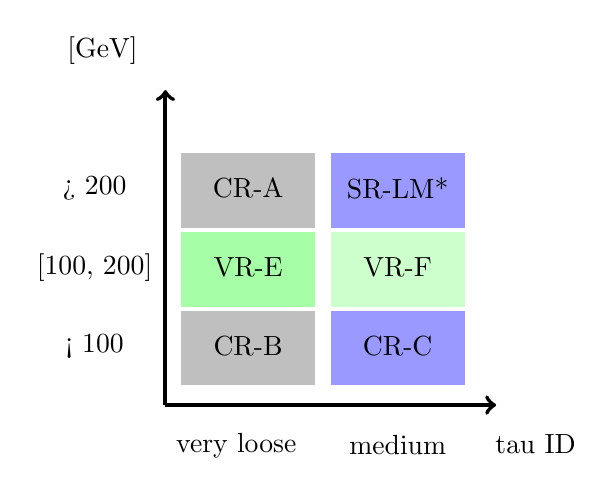
\begin{tikzpicture}
		\draw[line width =1.5pt,->] (0,0) -- (4.2,0);
		\node[](A) at (4.7,-0.5) {tau ID};
		\draw[line width =1.5pt,->] (0,0) -- (0,4.0);
		\node[](B) at (-0.8,4.5) {\Summt [GeV]};
		\node[](D) at (0.9, -0.51) {very loose };
		\node[](D) at (2.95, -0.50) {medium };
		\fill[gray!50] (0.2,0.25) rectangle (1.9,1.2);
		\node[](E) at (1.05,0.75) {CR-B};
		\node[](F)  at (-0.9,0.75) {< 100};
		\fill[green!35] (0.2,1.25) rectangle (1.9,2.2);
		\node[](G) at (1.05,1.75) {VR-E};
		\node[](H)  at (-0.9,1.75) {[100, 200]};
		\fill[gray!50] (0.2,2.25) rectangle (1.9,3.2);
		\node[](I) at (1.05,2.75) {CR-A};
		\node[](J)  at (-0.9,2.75) {> 200};
		\fill[blue!40] (2.1,0.25) rectangle (3.8,1.2);
		\node[](K) at (2.95,0.75) {CR-C};
		\fill[green!20] (2.1,1.25) rectangle (3.8,2.2);
		\node[](L) at (2.95,1.75) {VR-F};
		\fill[blue!40] (2.1,2.25) rectangle (3.8,3.2);
		\node[](M) at (2.95,2.75) {SR-LM*};
		\end{tikzpicture} }}
		  \subfloat[High mass ABCD regions]{
		\centering
	\scalebox{0.9}{
		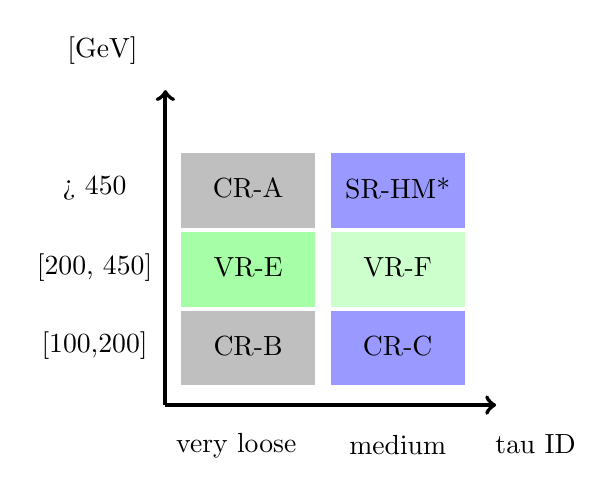
\begin{tikzpicture}
		\draw[line width =1.5pt,->] (0,0) -- (4.2,0);
		\node[](A) at (4.7,-0.5) {tau ID};
		\draw[line width =1.5pt,->] (0,0) -- (0,4.0);
		\node[](B) at (-0.8,4.5) {\Summt [GeV]};
		\node[](D) at (0.9, -0.51) {very loose };
		\node[](D) at (2.95, -0.50) {medium };
		\fill[gray!50] (0.2,0.25) rectangle (1.9,1.2);
		\node[](E) at (1.05,0.75) {CR-B};
		\node[](F)  at (-0.9,0.75) {[100,200]};
		\fill[green!35] (0.2,1.25) rectangle (1.9,2.2);
		\node[](G) at (1.05,1.75) {VR-E};
		\node[](H)  at (-0.9,1.75) {[200, 450]};
		\fill[gray!50] (0.2,2.25) rectangle (1.9,3.2);
		\node[](I) at (1.05,2.75) {CR-A};
		\node[](J)  at (-0.9,2.75) {> 450};
		\fill[blue!40] (2.1,0.25) rectangle (3.8,1.2);
		\node[](K) at (2.95,0.75) {CR-C};
		\fill[green!20] (2.1,1.25) rectangle (3.8,2.2);
		\node[](L) at (2.95,1.75) {VR-F};
		\fill[blue!40] (2.1,2.25) rectangle (3.8,3.2);
		\node[](M) at (2.95,2.75) {SR-HM*};
		\end{tikzpicture}}
}
\caption{ABCD region illustration for the low and high mass signal regions \label{fig:bkgestimation:QCD:sketch} Here only the cuts on \Summt and the tau-ID are shown.  $^*$ As described in section \ref{sec:analysis:sroptimisation},  further requirements on other kinematic variables are applied to define the signal regions}
\end{figure}

\begin{table}[ht!]
\centering
\footnotesize
\begin{tabular}{|c|c||c|c|}
\hline 
\textbf{CR-A} & \textbf{SR-LM} & \textbf{CR-A} & \textbf{SR-HM}\tabularnewline
\hline 
\hline 
$\geq$2 very loose or loose $\tau$'s & $\geq$2 medium $\tau$'s & $\geq$2 very loose or loose $\tau$'s & $\geq$2 medium $\tau$'s\tabularnewline
\textless{} 2 medium $\tau$'s & - & \textless{} 2 medium $\tau$'s & -\tabularnewline
$m_{Tsum}\geq200$ GeV & $m_{Tsum}\geq200$ GeV & $m_{Tsum}\geq450$ GeV & $m_{Tsum}\geq450$ GeV\tabularnewline
$\Delta\Phi(\tau_{1},\tau_{2})\geq1.5$ & $\Delta\Phi(\tau_{1},\tau_{2})\geq1.5$ & \Met $\geq$50 GeV & \Met $\geq$150 GeV\tabularnewline
\hline 
\hline 
\textbf{VR-E} & \textbf{VR-F} & \textbf{VR-E} & \textbf{VR-F}\tabularnewline
\hline 
\hline 
$\geq$2 very loose or loose $\tau$'s & $\geq$2 medium $\tau$'s & $\geq$2 very loose or loose $\tau$'s & $\geq$2 medium $\tau$'s\tabularnewline
\textless{} 2 medium $\tau$'s & - & \textless{} 2 medium $\tau$'s & -\tabularnewline
$m_{Tsum}$ $\in$ $[100,200]$ GeV & $m_{Tsum}$ $\in$ $[100,200]$ GeV & $m_{Tsum}$ $\in$ $[200,450]$ GeV & $m_{Tsum}$ $\in$ $[200,450]$ GeV\tabularnewline
$\Delta\Phi(\tau_{1},\tau_{2})\leq1.5$ & $\Delta\Phi(\tau_{1},\tau_{2})\leq1.5$ & \Met $\geq$50 GeV & \Met $\geq$50 GeV\tabularnewline
\hline 
\hline 
\textbf{CR-B} & \textbf{CR-C} & \textbf{CR-B} & \textbf{CR-C}\tabularnewline
\hline 
\hline 
$\geq$2 very loose or loose $\tau$'s & $\geq$2 medium $\tau$'s & $\geq$2 very loose or loose $\tau$'s & $\geq$2 medium $\tau$'s\tabularnewline
\textless{} 2 medium $\tau$'s & - & \textless{} 2 medium $\tau$'s & -\tabularnewline
$m_{Tsum}<100$ GeV & $m_{Tsum}<100$ GeV & $m_{Tsum}$ $\in$ $[100,200]$ GeV & $m_{Tsum}$ $\in$ $[100,200]$ GeV\tabularnewline
$\Delta\Phi(\tau_{1},\tau_{2})\leq1.5$ & $\Delta\Phi(\tau_{1},\tau_{2})\leq1.5$ & \Met $\geq$50 GeV & \Met $\geq$50 GeV\tabularnewline
\hline 
\end{tabular}
\caption{The multi-jet control region and validation region
  definitions for signal regions described in Table~\ref{tab:SRdef}.
  Only those requirements regarding the \Summt that are different in the CRs/VRs with
  respect to the SRs are listed. \label{tab:bkgestimation:QCD:table}}
\end{table}

%
%\begin{table}[ht!]
%\centering
%\footnotesize
%\smallskip
%\begin{tabular}{c|c}
%\toprule
%% AD------------------
%$\mathbf {CR-A~}$ & $\mathbf {SR-LM}$\\
%\hline
%$\ge$ 2 very loose or loose $\tau$s       & $\ge$ 2 medium $\tau$s (SS)   \\
%$<$ 2 medium $\tau$s     &      --      \\
%$m_{Tsum}\geq 200 \text{ GeV} $ &  $m_{Tsum}\geq 200 \text{ GeV} $      \\ %SumMtCut
%$\Delta \Phi(\tau_1,\tau_2) \geq 1.5 $ &  $\Delta \Phi(\tau_1,\tau_2) \geq 1.5 $ \\ %DeltaPhiCut
%\hline
%%EF---------------
%\hline
%$\mathbf {VR-E~}$ & $\mathbf {VR-F~}$ \\
%\hline                                                      \hline
%$\ge$ 2 very loose or loose $\tau$s       & $\ge$ 2 medium $\tau$s (SS)   \\
%$<$ 2 medium $\tau$s     &      --      \\
%$m_{Tsum}\in [100,200] \text{ GeV} $ &  $m_{Tsum}\in [100,200] \text{ GeV} $      \\ %SumMtCut
%$\Delta \Phi(\tau_1,\tau_2) \leq 1.5 $ &  $\Delta \Phi(\tau_1,\tau_2) \leq 1.5 $ \\ %DeltaPhiCut
%\hline
%% BC-----------------
%\hline
%$\mathbf {CR-B~}$ & $\mathbf {CR-C~}$ \\
%\hline                                                      \hline
%$\ge$ 2 very loose or loose $\tau$s       &  $\ge$ 2 medium $\tau$s (SS)   \\
%$<$ 2 medium $\tau$s     &      --      \\
%$m_{Tsum}< 100 \text{ GeV} $ &  $m_{Tsum}< 100 \text{ GeV} $      \\ %SumMtCut
%$\Delta \Phi(\tau_1,\tau_2) \leq 1.5 $ &  $\Delta \Phi(\tau_1,\tau_2) \leq 1.5 $ \\ %DeltaPhiCut
%\hline
%\bottomrule
%\end{tabular}
%\smallskip
%\begin{tabular}{c|c}
%\toprule
%% AD------------------
%$\mathbf {CR-A~}$ & $\mathbf {SR-HM}$\\
%\hline
%$\ge$ 2 very loose or loose $\tau$s       & $\ge$ 2 medium $\tau$s (SS)   \\
%$<$ 2 medium $\tau$s     &      --      \\
%$m_{Tsum}\geq 450 \text{ GeV} $ &  $m_{Tsum}\geq 450 \text{ GeV} $      \\ %SumMtCut
%$E_T^\text{miss} \geq 50 \text{ GeV} $ & $E_T^\text{miss} \geq 150 \text{ GeV} $ \\ %met cut
%\hline
%%EF---------------
%\hline
%$\mathbf {VR-E~}$ & $\mathbf {VR-F~}$\\
%\hline                                                      \hline
%$\ge$ 2 very loose or loose $\tau$s       & $\ge$ 2 medium $\tau$s (SS)   \\
%$<$ 2 medium $\tau$s     &      --      \\
%$m_{Tsum}\in [200,450] \text{ GeV} $ &  $m_{Tsum}\in [200,450] \text{ GeV} $      \\ %SumMtCut
%$E_T^\text{miss} \geq 50 \text{ GeV} $ & $E_T^\text{miss} \geq 50 \text{ GeV} $ \\ %met cut
%\hline
%% BC-----------------
%\hline
%$\mathbf {CR-B~}$ & $\mathbf {CR-C~}$ \\
%\hline                                                      \hline
%$\ge$ 2 very loose or loose $\tau$s       &  $\ge$ 2 medium $\tau$s (SS)   \\
%$<$ 2 medium $\tau$s     &      --      \\
%$m_{Tsum} \in [100,200] \text{ GeV} $ &  $m_{Tsum} \in [100,200] \text{ GeV} $      \\ %SumMtCut
%$E_T^\text{miss} \geq 50 \text{ GeV} $ & $E_T^\text{miss} \geq 50 \text{ GeV} $ \\ %met cut
%\hline
%\bottomrule
%\end{tabular}
%\caption{The multi-jet control region and validation region
%  definitions for signal regions described in Table~\ref{tab:SRdef}.
%  Only those requirements regarding the \Summt that are different in the CRs/VRs with
%  respect to the SRs are listed. \label{tab:bkgestimation:QCD:table}}
%\end{table}

The multi-jet (MJ) contribution in CR-B and CR-C is obtained from the data yields in the respective regions,  with all other background contributions from Monte Carlo simulation subtracted;

\begin{align}
N^{MJ}_{CR-B/C} =  N^{data}_{CR-B/C} - N^{MC}_{CR-B/C} 
\end{align}

a transfer factor is extracted from the yields in CR-B and CR-C to extrapolate the multi-jet contribution to the medium ID validation and signal regions (VR-F and SR). 

\begin{align}
TF = \frac{N^{MJ}_{CR-C}}{N^{MJ}_{CR-B}}
\label{eq:bkgestimation:TF}
\end{align}

The systematic uncertainty on the transfer factor is estimated in the validation regions using formula \eqref{eq:bkgestimation:deltaTF} and is visualised in Figure \ref{fig:bkgestimation:ABCD:TF}.

\begin{align}
\Delta(TF)_{sys} =  | \frac{N^{MJ}_{CR-C}}{N^{MJ}_{CR-B}} - \frac{N^{MJ}_{VR-F}}{N^{MJ}_{VR-E}} | \label{eq:bkgestimation:deltaTF}
\end{align}

\begin{figure}[!htpb]
  \centering
%\subfloat[Low Mass]{\includegraphics[width=0.45\textwidth]{figures/C1N2SS/ABCD_closures/TF_SumMt_asymMT2False.pdf}}
\subfloat[Low Mass]{\includegraphics[width=0.45\textwidth]{figures/C1N2SS/ABCD_closures_noATLAS/TF_SumMtADT_asymMT2False.pdf}}
%\subfloat[High Mass]{\includegraphics[width=0.45\textwidth]{figures/C1N2SS/ABCD_closures/TF_SumMt_ditauMETMT2False.pdf}}
\subfloat[High Mass]{\includegraphics[width=0.45\textwidth]{figures/C1N2SS/ABCD_closures_noATLAS/TF_SumMtDTM_ditauMETMT2False.pdf}}
\caption{Dependency of the transfer factor on \Summt for low mass and high mass regions. Highlighted in the lower panel in red is the nominal used transfer factor value. All uncertainties are statistical only. \label{fig:bkgestimation:ABCD:TF}}
\end{figure}

%%----- result
The multi-jet yield in the signal region is then given by the multi-jet contribution in CR-A (given through data subtracted by other \ac{SM} contributions from Monte Carlo simulation) multiplied by the transfer factor with additional cuts.
The results of the ABCD method are summarised in Table
\ref{tab:bkgestimation:ABCDresults}. The SM predictions are in agreement with
the observed data counts in the multi-jet validation regions, as shown in Table \ref{tab:bkgestimation:VRFresults}.
%The systematic uncertainties of the ABCD method are discussed in
%Section \ref{sec:syst_ABCD}.

%\begin{table}
%\centering
%\tiny
%  \begin{tabular}{c|c|c|c|c|c|c|c|c}
%  \hline
%  & Sample & CR-B & CR-C & VR-E & CR-A & T=C/B & multi-jet in VR-F & multi-jet in SR-D\tabularnewline
%  \hline
%  \hline
%  \multirow{7}{*}{LM} & \textbf{Data} & \textbf{585} & \textbf{65} & \textbf{356} & \textbf{1505} & \multirow{2}{*}{} & \multirow{7}{*}{$19.55 \pm 1.13$} & \multirow{7}{*}{$0.94\pm0.27$}\tabularnewline
%%  \cline{2-2}
%   & $Z$+ jets & $11.70\pm2.11$ & $25.92\pm2.70$ & $3.62\pm1.06$ & $32.85\pm11.07$ &  &  & \tabularnewline
%  \cline{2-2}
%   & $W$+ jets & $4.84\pm2.35$ & $3.29\pm0.96$ & $11.48\pm4.67$ & $32.21\pm10.06$ & $0.058$ &  & \tabularnewline
%  \cline{2-2}
%   & Multiboson & $0.80\pm0.38$ & $2.04\pm0.35$ & $1.20\pm0.40$ & $2.18\pm0.50$ & $\pm0.015$ &  & \tabularnewline
%  \cline{2-2}
%   & Top & $2.54\pm0.75$ & $0.16\pm0.27$ & $2.45\pm0.88$ & $5.24\pm0.93$ & $\pm0.020$ &  & \tabularnewline
%  \cline{2-2}
%   & Higgs & $0.13\pm0.04$ & $0.73\pm0.09$ & $0.09\pm0.05$ & $0.53\pm0.46$ & \multirow{2}{*}{} &  & \tabularnewline
%  \cline{2-2}
%   & \emph{Multi-jet} & $564.98\pm24.41$ & $32.86\pm8.57$ & $337.16\pm19.49$ & $1431.98\pm41.59$ &  &  & \tabularnewline
%  \hline
%  \hline
%  \multirow{7}{*}{HM} & \textbf{Data} & \textbf{2185} & \textbf{309} & \textbf{3651} & \textbf{14} & \multirow{2}{*}{} & \multirow{7}{*}{$283.10 \pm 7.738$} & \multirow{7}{*}{$-0.086\pm0.31$}\tabularnewline
%  \cline{2-2}
%   & $Z$+ jets & $30.81\pm7.41$ & $32.53\pm10.81$ & $56.12\pm17.74$ & $2.64\pm1.37$ &  &  & \tabularnewline
%  \cline{2-2}
%   & $W$+ jets & $178.87\pm51.40$ & $74.13\pm15.33$ & $248.68\pm64.10$ & $6.35\pm2.58$ & $0.086$ &  & \tabularnewline
%  \cline{2-2}
%   & Multiboson & $6.03\pm0.87$ & $18.35\pm0.97$ & $14.42\pm1.44$ & $0.83\pm0.29$ & $\pm0.014$ &  & \tabularnewline
%  \cline{2-2}
%   & Top & $20.73\pm2.01$ & $14.38\pm1.53$ & $39.23\pm2.72$ & $2.10\pm0.57$ & $\pm0.011$ &  & \tabularnewline
%  \cline{2-2}
%   & Higgs & $0.53\pm0.38$ & $1.27\pm0.58$ & $0.71\pm0.47$ & $0.01\pm0.00$ & \multirow{2}{*}{} &  & \tabularnewline
%  \cline{2-2}
%   & \emph{Multi-jet} & $1948.04\pm69.90$ & $168.34\pm25.78$ & $3291.83\pm89.91$ & $2.07\pm4.79$ &  &  & \tabularnewline
%  \hline
%  \end{tabular}
%  \caption{Monte Carlo  backgrounds in the ABCD regions of the signal
%  regions defined in Table \ref{tab:SRdef}. The uncertainties given
%  on the transfer factor are both statistical and systematic
%  uncertainties. \label{tab:bkgestimation:ABCDresults} }
%\end{table}

\begin{table}
\centering {\tiny{}}%
\begin{tabular}{|c|c|c|c|c|c|c|c|c|}
\hline 
\multirow{2}{*}{} & \multirow{2}{*}{\textbf{\tiny{}Sample }} & \multirow{2}{*}{\textbf{\tiny{}CR-B }} & \multirow{2}{*}{\textbf{\tiny{}CR-C }} & \multirow{2}{*}{\textbf{\tiny{}VR-E }} & \multirow{2}{*}{\textbf{\tiny{}CR-A }} & \multirow{2}{*}{\textbf{\tiny{}T=C/B}{\tiny{} }} & \textbf{\tiny{}multi-jet } & \textbf{\tiny{}multi-jet }\tabularnewline
 &  &  &  &  &  &  & \textbf{\tiny{}in VR-F } & \textbf{\tiny{}in SR-C1N2SS}\tabularnewline
\hline 
\hline 
\multirow{7}{*}{\textbf{\tiny{}LM}} & \textbf{\tiny{}Data}{\tiny{} } & \textbf{\tiny{}585}{\tiny{} } & \textbf{\tiny{}65}{\tiny{} } & \textbf{\tiny{}356}{\tiny{} } & \textbf{\tiny{}1505}{\tiny{} } & \multirow{2}{*}{} & \multirow{7}{*}{{\tiny{}$19.55\pm1.13$}} & \multirow{7}{*}{{\tiny{}$0.94\pm0.27$}}\tabularnewline
\cline{2-6} \cline{3-6} \cline{4-6} \cline{5-6} \cline{6-6} 
 & {\tiny{}$Z$+ jets } & {\tiny{}$11.70\pm2.11$ } & {\tiny{}$25.92\pm2.70$ } & {\tiny{}$3.62\pm1.06$ } & {\tiny{}$32.85\pm11.07$ } &  &  & \tabularnewline
\cline{2-6} \cline{3-6} \cline{4-6} \cline{5-6} \cline{6-6} 
 & {\tiny{}$W$+ jets } & {\tiny{}$4.84\pm2.35$ } & {\tiny{}$3.29\pm0.96$ } & {\tiny{}$11.48\pm4.67$ } & {\tiny{}$32.21\pm10.06$ } & {\tiny{}$0.058$ } &  & \tabularnewline
\cline{2-6} \cline{3-6} \cline{4-6} \cline{5-6} \cline{6-6} 
 & {\tiny{}Multi-boson } & {\tiny{}$0.80\pm0.38$ } & {\tiny{}$2.04\pm0.35$ } & {\tiny{}$1.20\pm0.40$ } & {\tiny{}$2.18\pm0.50$ } & {\tiny{}$\pm0.015$ } &  & \tabularnewline
\cline{2-6} \cline{3-6} \cline{4-6} \cline{5-6} \cline{6-6} 
 & {\tiny{}Top } & {\tiny{}$2.54\pm0.75$ } & {\tiny{}$0.16\pm0.27$ } & {\tiny{}$2.45\pm0.88$ } & {\tiny{}$5.24\pm0.93$ } & {\tiny{}$\pm0.020$ } &  & \tabularnewline
\cline{2-6} \cline{3-6} \cline{4-6} \cline{5-6} \cline{6-6} 
 & {\tiny{}Higgs } & {\tiny{}$0.13\pm0.04$ } & {\tiny{}$0.73\pm0.09$ } & {\tiny{}$0.09\pm0.05$ } & {\tiny{}$0.53\pm0.46$ } & \multirow{2}{*}{} &  & \tabularnewline
\cline{2-6} \cline{3-6} \cline{4-6} \cline{5-6} \cline{6-6} 
 & \emph{\tiny{}Multi-jet}{\tiny{} } & {\tiny{}$564.98\pm24.41$ } & {\tiny{}$32.86\pm8.57$ } & {\tiny{}$337.16\pm19.49$ } & {\tiny{}$1431.98\pm41.59$ } &  &  & \tabularnewline
\hline 
\multirow{7}{*}{\textbf{\tiny{}HM}} & \textbf{\tiny{}Data}{\tiny{} } & \textbf{\tiny{}2185}{\tiny{} } & \textbf{\tiny{}309}{\tiny{} } & \textbf{\tiny{}3651}{\tiny{} } & \textbf{\tiny{}14}{\tiny{} } & \multirow{2}{*}{} & \multirow{7}{*}{{\tiny{}$283.10\pm7.738$}} & \multirow{7}{*}{{\tiny{}$-0.086\pm0.31$}}\tabularnewline
\cline{2-6} \cline{3-6} \cline{4-6} \cline{5-6} \cline{6-6} 
 & {\tiny{}$Z$+ jets } & {\tiny{}$30.81\pm7.41$ } & {\tiny{}$32.53\pm10.81$ } & {\tiny{}$56.12\pm17.74$ } & {\tiny{}$2.64\pm1.37$ } &  &  & \tabularnewline
\cline{2-6} \cline{3-6} \cline{4-6} \cline{5-6} \cline{6-6} 
 & {\tiny{}$W$+ jets } & {\tiny{}$178.87\pm51.40$ } & {\tiny{}$74.13\pm15.33$ } & {\tiny{}$248.68\pm64.10$ } & {\tiny{}$6.35\pm2.58$ } & {\tiny{}$0.086$ } &  & \tabularnewline
\cline{2-6} \cline{3-6} \cline{4-6} \cline{5-6} \cline{6-6} 
 & {\tiny{}Multi-boson } & {\tiny{}$6.03\pm0.87$ } & {\tiny{}$18.35\pm0.97$ } & {\tiny{}$14.42\pm1.44$ } & {\tiny{}$0.83\pm0.29$ } & {\tiny{}$\pm0.014$ } &  & \tabularnewline
\cline{2-6} \cline{3-6} \cline{4-6} \cline{5-6} \cline{6-6} 
 & {\tiny{}Top } & {\tiny{}$20.73\pm2.01$ } & {\tiny{}$14.38\pm1.53$ } & {\tiny{}$39.23\pm2.72$ } & {\tiny{}$2.10\pm0.57$ } & {\tiny{}$\pm0.011$ } &  & \tabularnewline
\cline{2-6} \cline{3-6} \cline{4-6} \cline{5-6} \cline{6-6} 
 & {\tiny{}Higgs } & {\tiny{}$0.53\pm0.38$ } & {\tiny{}$1.27\pm0.58$ } & {\tiny{}$0.71\pm0.47$ } & {\tiny{}$0.01\pm0.00$ } & \multirow{2}{*}{} &  & \tabularnewline
\cline{2-6} \cline{3-6} \cline{4-6} \cline{5-6} \cline{6-6} 
 & \emph{\tiny{}Multi-jet}{\tiny{} } & {\tiny{}$1948.04\pm69.90$ } & {\tiny{}$168.34\pm25.78$ } & {\tiny{}$3291.83\pm89.91$ } & {\tiny{}$2.07\pm4.79$ } &  &  & \tabularnewline
\hline 
\end{tabular}{\tiny{}\caption{Monte Carlo backgrounds in the ABCD regions of the signal regions
defined in Table \ref{tab:SRdef}. The uncertainties given on the
transfer factor are  statistical followed by systematic uncertainties.
\label{tab:bkgestimation:ABCDresults} }
}
\end{table}


\begin{table}
\centering
\begin{tabular}{|c|c|c|}
\hline
Sample & VRF-LM& VRF-HM\\
\hline
\hline
W+jets & $1.35\pm0.88$ & $149.75\pm42.98$\\
\hline
Z+jets & $9.30\pm1.30$ & $36.82\pm19.62$\\
\hline
top & $0.99\pm0.48$ & $19.78\pm1.85$\\
\hline
Muliboson & $1.47\pm0.35$ & $26.31\pm1.2$\\
\hline
Higgs & $0.25\pm0.06$ & $3.16\pm1.13$\\
\hline
multi-jet & $19.55 \pm 1.13$ & $283.10 \pm 7.73$\\
\hline
\hline
SM total & $32.92 \pm 2.02$ & $518.92 \pm 47.94$\\
\hline
\textbf{Data} & \textbf{40} & \textbf{484}\\
\hline
\end{tabular}
\caption{Event yields in VR-F-LM and VR-F-HM. Only statistical
  uncertainties are included in the multi-jet 
  yield.  \label{tab:bkgestimation:VRFresults}%\textcolor{red}{Check ABCD validation, large disagreement}
}
\end{table}

%\textcolor{red}{distribution for Direct Stau validations to be added!}
In Figure \ref{fig:QCD-VR-LowMass-ss} (Figure \ref{fig:QCD-VR-highMass-ss}) ,
distributions of the relevant kinematic variables are shown for data,
SM expectations and illustrative SUSY benchmark models for the
multi-jet validation regions VR-F-LM (VR-F-HM).  The multi-jet contribution in VR-F is given through the multijet contribution in VR-E (as data subtracted by other \ac{SM} contributions) times the transfer factor as defined in equation \eqref{eq:bkgestimation:TF}. The signal contamination in VR-F-LM is below 10\%,  in VR-F-HM below 30\%. The SM background distributions are taken from MC
simulation, except for the multi-jet contribution, which is estimated using the ABCD method
described above. 
The distributions include statistical and systematic error on the ABCD method added in quadrature.
Reasonable data and SM agreement are observed within uncertainty and show good extrapolation in \Mttwomax.

%--------------------------------------------------------------------
\begin{figure}[!htpb]
\centering
  \subfloat[]{\includegraphics[width=0.45\textwidth]{figures/UpdatedThesisFigures/VRFLM_Prefit_noATLAS/asymVRF_wDPhiOnly_noLLV_mt2maxvrfL.pdf}}
  \subfloat[]{\includegraphics[width=0.45\textwidth]{figures/UpdatedThesisFigures/VRFLM_Prefit_noATLAS/VRFLM_met.pdf}}\\
 \subfloat[]{\includegraphics[width=0.45\textwidth]{figures/UpdatedThesisFigures/VRFLM_Prefit_noATLAS/asymVRF_wDPhiOnly_noLLV_SumMtTauVRFLM.pdf}}
   \subfloat[]{\includegraphics[width=0.45\textwidth]{figures/UpdatedThesisFigures/VRFLM_Prefit_noATLAS/asymVRF_wDPhiOnly_noLLV_mvisTauTauSRH_improved.pdf}}\\
%  \subfloat[]{\includegraphics[width=0.45\textwidth]{figures/C1N2SS/ABCD_low/asymVRF_wDPhiOnly_noLLV_signaljets.pdf}}
 % \subfloat[]{\includegraphics[width=0.45\textwidth]{figures/C1N2SS/ABCD_low/asymVRF_wDPhiOnly_noLLV_deltaPhiTau1Met.pdf}}\\
  \subfloat[]{\includegraphics[width=0.45\textwidth]{figures/UpdatedThesisFigures/VRFLM_Prefit_noATLAS/asymVRF_wDPhiOnly_noLLV_tau1PtVRFLtrigLim_improved.pdf}}
  \subfloat[]{\includegraphics[width=0.45\textwidth]{figures/UpdatedThesisFigures/VRFLM_Prefit_noATLAS/asymVRF_wDPhiOnly_noLLV_tau2PtSRH_improved.pdf}}
  %\subfloat[]{\includegraphics[width=0.45\textwidth]{figures/C1N2SS/ABCD_low/asymVRF_wDPhiOnly_noLLV_nbjets.pdf}}
  \caption{Data/MC distributions in VR-F-LM, the uncertainty band includes statistical and systematic uncertainties. 
\label{fig:QCD-VR-LowMass-ss}}
\end{figure} %\addtocounter{figure}{-1}

\begin{figure}[!htpb]
\centering
  \subfloat[]{\includegraphics[width=0.45\textwidth]{figures/UpdatedThesisFigures/VRFHM_Prefit_noATLAS/ditauMETVRFSumMtlowMet_plateau_mt2maxvrfH_improved.pdf}}
  \subfloat[]{\includegraphics[width=0.45\textwidth]{figures/UpdatedThesisFigures/VRFHM_Prefit_noATLAS/ditauMETVRFSumMtlowMet_plateau_metVRFH.pdf}}\\
   \subfloat[]{\includegraphics[width=0.45\textwidth]{figures/UpdatedThesisFigures/VRFHM_Prefit_noATLAS/ditauMETVRFSumMtlowMet_plateau_SumMtTauVRFHM_5b.pdf}}
  \subfloat[]{\includegraphics[width=0.45\textwidth]{figures/UpdatedThesisFigures/VRFHM_Prefit_noATLAS/ditauMETVRFSumMtlowMet_plateau_mvisTauTau100.pdf}}\\
  %\subfloat[]{\includegraphics[width=0.45\textwidth]{figures/C1N2SS/ABCD_high/ditauMETVRFSumMtlowMet_plateau_signaljets.pdf}}
  %\subfloat[]{\includegraphics[width=0.45\textwidth]{figures/C1N2SS/ABCD_high/ditauMETVRFSumMtlowMet_plateau_deltaPhiTau1Met.pdf}}\\
  \subfloat[]{\includegraphics[width=0.45\textwidth]{figures/UpdatedThesisFigures/VRFHM_Prefit_noATLAS/ditauMETVRFSumMtlowMet_plateau_tau1PtVRFH_improved.pdf}}
  \subfloat[]{\includegraphics[width=0.45\textwidth]{figures/UpdatedThesisFigures/VRFHM_Prefit_noATLAS/ditauMETVRFSumMtlowMet_plateau_tau2PtSRH_improved.pdf}}
 % \subfloat[]{\includegraphics[width=0.45\textwidth]{figures/C1N2SS/ABCD_high/ditauMETVRFSumMtlowMet_plateau_nbjets.pdf}}
  \caption{Data/MC distributions in VR-F-HM, the uncertainty band includes statistical and systematic uncertainties. 
\label{fig:QCD-VR-highMass-ss}}
\end{figure}

\pagebreak
\clearpage
\subsection{Estimation of W+jets background}
\label{sec:SS:Wjets}
%====================================================================================================
%==============================================W+jets estimation ==================================
%====================================================================================================
\FloatBarrier
The production of a W boson in association with a jet can enter a di-tau final state if one or more of the associated jets is misidentified as hadronic decaying tau lepton.  The W+jets background contributes to both low and high mass signal regions,  through moderate \Met contributions of the neutrinos in the W bosons decay and mismeasured \Met. 
A control and validation region targetting both signal regions is defined to estimate this background.  A summary of the requirements applied to define the regions is given in Table \ref{tab:bkgestimation:WCRVR}.
A final state with precisely one hadronically decaying tau lepton and one muon,  both with the same electric charge,  is selected to increase the available statistics. 
This final state targets to model events entering the signal regions with at least one fake tau,  replacing the prompt tau through a prompt muon. 
A veto on baseline electrons is applied to target the muon plus hadronic tau final state.
A veto on b-jets is used to constrain contributions from top related processes,  whereas a cut on the transverse mass of the muon is used to remove Z+jets contaminations. 
A lower cut on the \Met of 50 GeV is used to veto events with very close by muons and taus,  which accumulate at low \Met due to failed separation in overlap removal procedures.  A cut on the \Mttwo variable,  built with the muon and tau,  is required to achieve similar event structures and phase spaces to the signal regions. 
This mimics the kinematic restrictions on the two leading taus used in the signal regions.

\begin{table}[!htpb]
\centering
\begin{tabular}{|c|c|} \hline
$W$-CR                 & $W$-VR \\ \hline
\multicolumn{2}{|c|}{pass TrigHLT\_mu20\_iloose\_L1MU15 (2015) and HLT\_mu26\_ivarmedium (2016-2018)} \\
\multicolumn{2}{|c|}{$==$ 1 medium tau and 1 isolated muon (SS) } \\
\multicolumn{2}{|c|}{baseline electron veto}\\
\multicolumn{2}{|c|}{$b$-veto}\\
\multicolumn{2}{|c|}{$50 < \text{m}_{\text{T}}(\mu)<150\,\text{GeV}$}\\
\multicolumn{2}{|c|}{$\text{m}_{\text{T}}(\tau)+\text{m}_{\text{T}}(\mu)>80\,\text{GeV}$}\\
%\multicolumn{2}{|c|}{$ m_T(\mu) \in [50, 150]$}\\
%\multicolumn{2}{|c|}{$ m_T(\mu) + m_T(\tau_1) \geq 80 \text{ GeV}$}\\
\multicolumn{2}{|c|}{$E_T^\text{miss} > 50 \text{ GeV}$}\\
$m_{T2}(\mu,\tau) <  60 \text{ GeV}$ & $m_{T2}(\mu, \tau) \geq 60 \text{ GeV}$\\ \hline
\end{tabular}\caption{Wjets control and validation region definition \label{tab:bkgestimation:WCRVR}}
\end{table}

With the cuts specified in Table \ref{tab:bkgestimation:WCRVR},  control and validation regions with high statistics are constructed, with a breakdown of the background yields, estimated purely from Monte Carlo simulation, which can be seen in table \ref{tab:bkgestimation:WCRVRyields}.
The yield does not include systematic uncertainties.  Both control and validation region show a high purity in W+jets processes,  above 80$\%$ in both cases,  as shown in figure \ref{fig:bkgestimation:WCRVRpurity}.  The signal contamination in both regions is negligible(see Fig.  \ref{fig:SS:WCRVRcontamination}). Kinematic distributions in the W-CR and W-VR are shown in Figure \ref{fig:SS:WCR} and \ref{fig:bkgestimation:wvrmcdata}, respectively. 

\begin{table}
  \centering
\begin{tabular}{|c|c|c|}
\hline
Sample & W-CR & W-VR\tabularnewline
\hline
\hline
W+jets & $ 21005.90 \pm 880.74 $ & $ 5852.23 \pm 502.55 $\tabularnewline
\hline
Z+jets  & $ 2529.68 \pm 205.40 $& $ 737.16 \pm 90.34 $\tabularnewline
\hline
top & $ 1148.86 \pm 12.66 $ & $ 185.39 \pm 5.18 $\tabularnewline
\hline
Multiboson & $ 629.41 \pm 8.79 $ & $ 122.50 \pm 3.62 $\tabularnewline
\hline
Higgs & $ 20.70 \pm 3.31 $ & $ 5.49 \pm 1.72 $\tabularnewline
\hline
Multi-jet & $0.00\pm0.00$ & $0.00\pm0.00$\tabularnewline
\hline
\hline
SM total & $ 25334.55 \pm 904.51 $ & $ 6902.76 \pm 510.65 $\tabularnewline
\hline
\textbf{Data} & \textbf{$\mathbf{25728}$} & $\mathbf{6662}$\tabularnewline
\hline
\end{tabular}
\caption{Event yields in W+jets Control and Validation region. The shown uncertainties for SM backgrounds are the statistical
uncertainties only.  \label{tab:bkgestimation:WCRVRyields}}
\end{table}

\begin{figure}[!htpb]
\centering
  \includegraphics[width=0.95\textwidth]{figures/UpdatedThesisFigures/WCRVR_piechart.png}
  \caption{Background composition in W+jet Control and Validation region \label{fig:bkgestimation:WCRVRpurity}}\end{figure}


\begin{figure}[!htpb]
  \centering
  \subfloat[W-CR]{\includegraphics[width=0.49\textwidth]{figures/C1N2SS/WVRCR_muWeight/SigBkgTrue_QCDtrFalse_MjFalseWCR_public_wolowMt2_vetobaselineelec_met.Syst_bkup_nonumbers.pdf}}
  \subfloat[W-VR]{\includegraphics[width=0.49\textwidth]{figures/C1N2SS/WVRCR_muWeight/SigBkgTrue_QCDtrFalse_MjFalseWVR_public_vetobaselineelec_met.Syst_bkup_nonumbers.pdf}}
\caption{Signal contamination in percentage in W-CR and W-VR. \label{fig:SS:WCRVRcontamination}}
\end{figure}

\begin{figure}[!htpb]
\centering
  \subfloat[]{\includegraphics[width=0.45\textwidth]{figures/UpdatedThesisFigures_noATLAS/WCR_Prefit/singlemuWCR_public_wolowMt2_vetobaselineelec_met_emtmt2max_wcr.pdf}}
  \subfloat[]{\includegraphics[width=0.45\textwidth]{figures/UpdatedThesisFigures_noATLAS/WCR_Prefit/singlemuWCR_public_wolowMt2_vetobaselineelec_met_metVRFH.pdf}}\\
  \subfloat[]{\includegraphics[width=0.45\textwidth]{figures/UpdatedThesisFigures_noATLAS/WCR_Prefit/singlemuWCR_public_wolowMt2_vetobaselineelec_met_muon_MTwcrvr.pdf}}
 % \subfloat[]{\includegraphics[width=0.45\textwidth]{figures/C1N2SS/WVRCR/singlemuWCR_public_wolowMt2_vetobaselineelec_met_signaljets.pdf}}
  \subfloat[]{\includegraphics[width=0.45\textwidth]{figures/UpdatedThesisFigures_noATLAS/WCR_Prefit/singlemuWCR_public_wolowMt2_vetobaselineelec_met_SumMtTauMuwcrvrshorter_improved.pdf}}\\
  %\subfloat[]{\includegraphics[width=0.45\textwidth]{figures/C1N2SS/WVRCR/singlemuWCR_public_wolowMt2_vetobaselineelec_met_deltaPhiTau1Met.pdf}}\\
  \subfloat[]{\includegraphics[width=0.45\textwidth]{figures/UpdatedThesisFigures_noATLAS/WCR_Prefit/singlemuWCR_public_wolowMt2_vetobaselineelec_met_tau1PtVRFH_improved.pdf}}
  \subfloat[]{\includegraphics[width=0.45\textwidth]{figures/UpdatedThesisFigures_noATLAS/WCR_Prefit/singlemuWCR_public_wolowMt2_vetobaselineelec_met_mu1Ptwcrvr_improved.pdf}}
  %\subfloat[]{\includegraphics[width=0.45\textwidth]{figures/C1N2SS/WVRCR/singlemuWCR_public_wolowMt2_nbjets.pdf}}
 \caption{ Distributions of  relevant kinematic variables in the $W$-CR.
The SM backgrounds other than multi-jet production are estimated from MC simulation
and normalised to 139~\ifb.
The hatched bands represent the statistical uncertainties and systematic uncertainties discussed in \ref{sec:analysis:systematics}.
%  The hatched bands represent the combined statistical and systematic uncertainties on the total SM background.
%For illustration, the distributions of the SUSY reference points are also shown as dashed lines.
The lower panel shows the ratio of data to the SM background estimate. \label{fig:SS:WCR} 
}
% \caption{W+jets control region data/MC distributions \label{fig:SS:WCR}}
\end{figure}

\begin{figure}[!htpb]
\centering
  \subfloat[]{\includegraphics[width=0.49\textwidth]{figures/UpdatedThesisFigures/WVR_Prefit_noATLAS/singlemuWVR_public_vetobaselineelec_met_emtmt2max_wvr_improved.pdf}}
  \subfloat[]{\includegraphics[width=0.49\textwidth]{figures/UpdatedThesisFigures/WVR_Prefit_noATLAS/singlemuWVR_public_vetobaselineelec_met_metWCRVR.pdf}}\\
  \subfloat[]{\includegraphics[width=0.49\textwidth]{figures/UpdatedThesisFigures/WVR_Prefit_noATLAS/WVR_muonmt.pdf}}
  %\subfloat[]{\includegraphics[width=0.49\textwidth]{figures/C1N2SS/WVRCR/singlemuWVR_public_vetobaselineelec_met_signaljets.pdf}}
  \subfloat[]{\includegraphics[width=0.49\textwidth]{figures/UpdatedThesisFigures/WVR_Prefit_noATLAS/singlemuWVR_public_vetobaselineelec_met_SumMtTauMuwcrvrshorter_improved.pdf}}\\
  %\subfloat[]{\includegraphics[width=0.49\textwidth]{figures/C1N2SS/WVRCR/singlemuWVR_public_vetobaselineelec_met_deltaPhiTau1Met.pdf}}\\
  \subfloat[]{\includegraphics[width=0.49\textwidth]{figures/UpdatedThesisFigures/WVR_Prefit_noATLAS/singlemuWVR_public_vetobaselineelec_met_tau1PtVRFH_improved.pdf}}
  \subfloat[]{\includegraphics[width=0.49\textwidth]{figures/UpdatedThesisFigures/WVR_Prefit_noATLAS/singlemuWVR_public_vetobaselineelec_met_mu1Ptwcrvr_improved.pdf}}
  %\subfloat[]{\includegraphics[width=0.49\textwidth]{figures/C1N2SS/WVRCR/singlemuWVR_public_nbjets.pdf}}
  %\caption{W+jets control region data/MC distributions \label{fig:SS:WVR}}
\caption{ Distributions of  relevant kinematic variables in the $W$-VR. The SM backgrounds other than multi-jet production are estimated from MC simulation and normalised to 139~\ifb.
The hatched bands represent the statistical uncertainties and systematic uncertainties discussed in \ref{sec:analysis:systematics}.
%   The hatched bands represent the combined statistical and systematic uncertainties on the total SM background.
%For illustration, the distributions of the SUSY reference points are also shown as dashed lines.
The lower panel shows the ratio of data to the SM background estimate. \label{fig:bkgestimation:wvrmcdata} 
}
\end{figure}

\pagebreak
\clearpage

%================================================================================================
%==============================================Top estimation =======================================
%=================================================================================================
\subsection{Top background estimation}
\label{sec:SS:Top}
\FloatBarrier
Top-related processes are a dominant background contribution, especially in SR-C1N2SS-HM (with around 35\% of the overall background expectation, as given in \ref{tab:SS:SRyields}). To estimate this background, a data-driven approach is used in the high mass scenario, using a control region (TCR-HM) to extract a normalisation factor. This is validated in a high mass Top validation region (TVR-HM).  The kinematic cuts used to define these regions can be seen in table \ref{tab:SS:TopVRs}, where the tau identification working point has been lowered to increase the available statistics.
A lower $E_T^\text{miss}$ requirement is applied to reduce the contribution of multi-jet processes.

\begin{table}[!htpb]
\centering
\begin{tabular}{|c|c|} \hline
TCR-HM & TVR-HM \\ \hline
\multicolumn{2}{|c|}{$n_{\text{at least very loose taus}} \geq 2$}\\
\multicolumn{2}{|c|}{$n_{\text{at least loose taus}} \geq 1$}\\
\multicolumn{2}{|c|}{$n_{\text{medium taus}} < 2$}\\
\multicolumn{2}{|c|}{$n_{BJets} \geq 1$}\\ \hline
\multicolumn{2}{|c|}{di-tau plus met trigger}\\
 \multicolumn{2}{|c|}{$E_T^\text{miss} \geq 150 \text{ GeV} $}\\
$m_{Tsum}\leq 400 \text{ GeV} $ & $m_{Tsum}\geq 400 \text{ GeV} $\\ \hline
\end{tabular}
\caption{Definition of Top Validation and Control regions \label{tab:SS:TopVRs}}
\end{table}

An overview of the event yields is shown in Table \ref{tab:SS:TopYields}, with a visualisation of the background contributions in the validation and control regions in Figure \ref{fig:SS:TopComp}.

\begin{table}[htpb!]
  \centering
\begin{tabular}{|c|c|c|}
\hline
\textbf{Sample} & \textbf{TCR-HM} & \textbf{TVR-HM}\tabularnewline
\hline
\hline
$W$+jets    &  $ 13.23 \pm 1.74 $ &  $ 1.06 \pm 0.31 $ \tabularnewline
\hline
$Z$+ jets   &  $ 4.31 \pm 0.90  $ & $ 0.81 \pm 0.43 $ \tabularnewline
\hline
top         &  $ 104.49 \pm 4.04 $ & $ 16.97 \pm 1.58 $         \tabularnewline
\hline
Multiboson  &  $ 3.13 \pm 0.92 $   & $ 0.22 \pm 0.08 $\tabularnewline
\hline
Higgs       &  $ 0.98 \pm 0.04 $   & $ 0.13 \pm 0.01 $      \tabularnewline
\hline
multi-jet & $0.00\pm0.00$ & $0.00\pm0.00$ \tabularnewline
\hline
\hline
SM total & $ 126.13 \pm 4.58 $ & $ 19.20 \pm 1.66  $ \tabularnewline
\hline
%\textbf{Data} & \textbf{96} & \textbf{12} \tabularnewlines
\textbf{Data} & \textbf{96} & $\mathbf{12}$\tabularnewline
\hline
\end{tabular}
\caption{Event yields of TCR-HM, TVR-HM \label{tab:SS:TopYields}. All uncertainties are statistical only.}
\end{table}

\begin{figure}[!htpb]
\centering
%  \subfloat[]{\includegraphics[width=0.49\textwidth]{figures/C1N2SS/TopVR/TopVRLowMass_pie19v04.png}}
\includegraphics[width=0.95\textwidth]{figures/UpdatedThesisFigures/TCRVRpiechart.png}
  \caption{Process composition in Top Control and Validations \label{fig:SS:TopComp}}
\end{figure} %\addtocounter{figure}{-1}

An overview of the signal contamination in percentage points in the top validation and control regions is shown in \ref{fig:SS:SigContTop}. The signal points with high contamination have been already excluded in a previous publication, using opposite-sign tau final states discussed in \cite{DiTauC1N2_2018}.

\begin{figure}[!htpb]
\centering
%  \subfloat[TopVRLowMass]{\includegraphics[width=0.49\textwidth]{figures/C1N2SS/TopVR/SigBkgTrue_QCDtrTrue_MjFalseTopVR_onlyB_Incrmet_veryLoose_highMet_sigTaus.Syst.pdf}}
  \subfloat[TCR-HM]{\includegraphics[width=0.49\textwidth]{figures/C1N2SS/TopVR_new/SigBkgTrue_QCDtrTrue_MjFalseTopbasic2_veryloose_CR_sigTaus_400.Syst_improved.pdf}}
  \subfloat[TVR-HM]{\includegraphics[width=0.49\textwidth]{figures/C1N2SS/TopVR_new/SigBkgTrue_QCDtrTrue_MjFalseTopbasic2_veryloose_VR_sigTaus_400.Syst_improved.pdf}}
  \caption{Signal contamination of high mass Top CR and VR in percent \label{fig:SS:SigContTop} }
\end{figure}%\addtocounter{figure}{-1}

\begin{figure}[!htpb]
\centering
  \subfloat[]{\includegraphics[width=0.49\textwidth]{figures/UpdatedThesisFigures_noATLAS/TCR/ditauMETTopbasic2_veryloose_CR_sigTaus_400_mt2max_improved.pdf}}
  \subfloat[]{\includegraphics[width=0.49\textwidth]{figures/UpdatedThesisFigures_noATLAS/TCR/ditauMETTopbasic2_veryloose_CR_sigTaus_400_metTCR.pdf}}\\
  \subfloat[]{\includegraphics[width=0.49\textwidth]{figures/UpdatedThesisFigures_noATLAS/TCR/ditauMETTopbasic2_veryloose_CR_sigTaus_400_mvisTauTau70_improved.pdf}}
  \subfloat[]{\includegraphics[width=0.49\textwidth]{figures/UpdatedThesisFigures_noATLAS/TCR/TCR_nsignaljets.pdf}}\\
  \subfloat[\label{TopCRsumt}]{\includegraphics[width=0.49\textwidth]{figures/UpdatedThesisFigures_noATLAS/TCR/TCR_mtsum.pdf}}
 % \subfloat[]{\includegraphics[width=0.49\textwidth]{figures/C1N2SS/TopVR_new/ditauMETTopbasic2_veryloose_CR_deltaPhiTau1Met.pdf}}
  \subfloat[]{\includegraphics[width=0.49\textwidth]{figures/UpdatedThesisFigures_noATLAS/TCR/ditauMETTopbasic2_veryloose_CR_sigTaus_400_tau1PtVRFH_improved.pdf}}\\
  \caption{Top High mass control region data/MC distributions. The hatched band is including the statistical and systematic uncertainties. \label{fig:bkgestimation:topccalermcdata} }
\end{figure}


\begin{figure}[!htpb]
\centering
  \subfloat[]{\includegraphics[width=0.49\textwidth]{figures/UpdatedThesisFigures/TVR_noATLAS/TVR_mt2max_improved.pdf}}
  \subfloat[]{\includegraphics[width=0.49\textwidth]{figures/UpdatedThesisFigures/TVR_noATLAS/TVR_met_improved.pdf}}\\
  \subfloat[]{\includegraphics[width=0.49\textwidth]{figures/UpdatedThesisFigures/TVR_noATLAS/TVR_mvis.pdf}}
  \subfloat[]{\includegraphics[width=0.49\textwidth]{figures/UpdatedThesisFigures/TVR_noATLAS/TVR_signaljets_improved.pdf}}\\
  \subfloat[]{\includegraphics[width=0.49\textwidth]{figures/UpdatedThesisFigures/TVR_noATLAS/TVR_mtsum_improved.pdf}}
  %\subfloat[]{\includegraphics[width=0.49\textwidth]{figures/C1N2SS/TopVR_new/ditauMETTopbasic2_veryloose_VR_deltaPhiTau1Met.pdf}}
  \subfloat[]{\includegraphics[width=0.49\textwidth]{figures/UpdatedThesisFigures/TVR_noATLAS/TVR_tau1pt_improved.pdf}}\\
  \caption{Top High mass validation region data/MC distributions. The hatched band is including the statistical and systematic uncertainty. \label{fig:bkgestimation:topvrmcdata}}
\end{figure} %\addtocounter{figure}{-1}

A downward trend in the data with respect to Monte Carlo simulation can be observed in some variables in Figure \ref{fig:bkgestimation:topccalermcdata} and \ref{fig:bkgestimation:topvrmcdata} of the T-CR and T-VR,  most dominantly in Figure \ref{TopCRsumt},  showing the $m_T(\tau_1)+m_T(\tau_2)$ distribution in the high mass top control region.
This shift in the Monte Carlo simulation agreement is due to a changing composition of the top contributions.  Towards higher transverse masses,  a slight increase in events with at least two fake taus can be observed.  Fake taus are poorly modelled in Monte Carlo and are leading to an overestimation of the Monte Carlo with respect to data. 
This trend is broken down in Figure \ref{fig:analysis:TopCRVRmtsum}, showing an inclusive $m_T(\tau_1)+m_T(\tau_2)$ distribution,  with all requirements from Table \ref{tab:SS:TopVRs},  except the $m_T(\tau_1)+m_T(\tau_2)$ cut separating the control and validation regions.
The analysis decomposing the top contribution based on the number of fake,  non-prompt tau leptons is done using truth information of the Monte Carlo generators, providing information of the generated process before detector simulation.
As can be seen,  the previous observed downward trends in data can be related to an increase in the top contribution with at least two fake taus. 
The cut in $m_T(\tau_1)+m_T(\tau_2)$ separating the control and validation region at 400 GeV has been chosen to enhance the two fake tau composition in the control region,  while still retaining enough background statistics in the validation region.  A breakdown of the top background composition in the high mass signal region as well as T-CR and T-VR is given in Table \ref{tab:app:c1n2ss:topbreakdownhigh}. 

\begin{figure}
\centering
\includegraphics[width=0.7\linewidth]{figures/171221_includeNoFakes/FakeContr_SumMt50_ditauMETMT2False.pdf}
\caption{Breakdown of the top compositions in the top control and validation region \label{fig:analysis:TopCRVRmtsum}}
\end{figure}

\begin{table}
  \centering
\begin{tabular}{|cc|c|c|c|}
\hline
\multicolumn{2}{|c|}{} & \textbf{SR-HM} & \textbf{TCR-HM} & \textbf{TVR-HM}\tabularnewline
\hline
\hline
\multicolumn{2}{|c|}{\textbf{all Top}} & \textbf{$\mathbf{0.84\pm0.36}$} & $104.49\pm4.04$ & $16.97\pm1.58$\tabularnewline
\hline
\hline
 & =0 fakes & $0.028\pm0.014$ & $14.89\pm1.49$ & $1.71\pm0.47$\tabularnewline
\hline
 & ==1 fake & $0.49\pm0.28$ & $81.14\pm3.58$ & $8.87\pm1.15$\tabularnewline
\hline
 & \textgreater =2 fakes & $0.319\pm0.23$ & $8.46\pm1.12$ & $6.39\pm0.98$\tabularnewline
\hline
\hline
\multicolumn{2}{|c|}{\textbf{ttbar}} & $0.61\pm0.31$ & $91.00\pm3.71$ & $15.67\pm1.53$\tabularnewline
\hline
\hline
 & =0 fakes & -- & $11.80\pm1.31$ & $1.52\pm0.47$\tabularnewline
\hline
 & ==1 fake & $0.30\pm0.21$ & $71.69\pm3.31$ & $8.20\pm1.11$\tabularnewline
\hline
 & \textgreater =2 fakes & $0.319\pm0.23$ & $7.51\pm1.04$ & $5.95\pm0.95$\tabularnewline
\hline
\multicolumn{2}{|c|}{\textbf{singletopWt}} & $0.19\pm0.19$ & $10.18\pm1.56$ & $0.56\pm0.29$\tabularnewline
\hline
\multicolumn{2}{|c|}{\textbf{ttV}} & $0.034\pm0.016$ & $1.98\pm0.17$ & $0.41\pm0.076$\tabularnewline
\hline
\multicolumn{2}{|c|}{\textbf{tZ}} & -- & $0.27\pm0.060$ & $0.014\pm0.027$\tabularnewline
\hline
\multicolumn{2}{|c|}{\textbf{singletopTchan}} & -- & $0.83\pm0.31$ & $0.28\pm0.20$\tabularnewline
\hline
\end{tabular}
\caption{Breakdown of top background contributions in the high mass regions by top processes and number of fake taus. Uncertainties included are statistical only. \label{tab:app:c1n2ss:topbreakdownhigh}}
\end{table}

\FloatBarrier
%===========================================
\subsection{Multi-boson background estimation}
%===========================================

Multi-boson processes are one of the leading contributions to SR-C1N2SS-HM  (as in \ref{tab:SRdef}). A validation region was designed to validate the modelling of these background processes from Monte Carlo simulation. 
To target the WZ and WW processes dominating the multi-boson contribution in the signal regions,  a selection of an opposite-sign muon pair and a hadronically decaying tau was used. This has been selected to target the contribution from real tau leptons, dominating this background process,  and estimate it through replacing real tau leptons with light leptons. 
As shown in Table \ref{tab:bkgestimation:MBVRdef}, a b-jet veto is used to suppress top-quark related backgrounds, a upper bound of $\Delta\phi (\tau,E_T^\text{miss}) \leq 1.75$ is used to restrict the
number of $Z$+jets events populating the multi-boson validation region. A summary of yields in the MBVR-SS is shown in Table \ref{tab:bkgestimation:MBVRyields}. 

\begin{table}[!htpb]
\centering
\begin{tabular}{|c|} \hline
MBVR-SS \\ \hline
\text{Two OS signal muons}\\
\text{== 1 signal tau}\\
\text{ b-Jet Veto}\\
$ E_T^{\text{miss}} \geq 100 \text{GeV} $\\
$\Delta\Phi(\tau,E_T^{\text{miss}}) \leq 1.75 $\\ \hline
\end{tabular}
\caption{MBVR-SS definition \label{tab:bkgestimation:MBVRdef}}
\end{table}

\begin{table}[!htpb]
\centering
\begin{tabular}{| c | r |}
\hline\hline
Sample& MBVR-SS\\ \hline
Multiboson & $ 144.22 \pm 1.96 $\\ \hline
Top & $ 33.30 \pm 2.13 $\\ \hline
Zjets & $ 16.44 \pm 29.32 $\\ \hline
Higgs & $ 4.30 \pm 1.26 $\\ \hline
Wjets & $ 0.08 \pm 0.08 $\\ \hline \hline
Total Bkg & $ 198.32 \pm 29.49 $ \\
Data& $ 200 $\\ \hline \hline
(325, 175) & $ 0.29 \pm 0.22 $ \\ \hline
(375, 175) & $ 1.07 \pm 0.39 $\\ \hline
\end{tabular}
\caption{Yields in MBVR \label{tab:bkgestimation:MBVRyields}. All uncertainties are statistical only.}
\end{table}

\begin{figure}[!htpb]
\subfloat[MBVR-SS Purity]{\includegraphics[width=0.49\textwidth]{figures/C1N2SS/MBVR_muWeight/MBVR_PieChart.png}}
\subfloat[MBVR-SS Signal contamination]{\includegraphics[width=0.49\textwidth]{figures/C1N2SS/MBVR_muWeight/SigCont_improved.pdf}}
\caption{Multiboson purity in MBVR-SS as well as signal contamination in \% \label{fig:bkgestimation:MBVR:PuritySigCont} }
\end{figure}
An overview of the background composition and multiboson purity, as well as the signal contamination in the region, is given in Figure \ref{fig:bkgestimation:MBVR:PuritySigCont}. A few selected kinematic variable distributions are given in Figure \ref{fig:bkgestimation:mbdatamc},  showing good agreement between the \ac{SM} expectation and data. 


\begin{figure}[!htpb]\centering
\subfloat[$\tau p_T$]{\includegraphics[width=0.49\textwidth]{figures/UpdatedThesisFigures_noATLAS/MBVR/MBVR_tau1pt_improved.pdf}}
\subfloat[$\mu_1 p_T$]{\includegraphics[width=0.49\textwidth]{figures/UpdatedThesisFigures_noATLAS/MBVR/singlemumultibosonmetPhimed_mu1Ptwcrvr_improved.pdf}}\\
\subfloat[$E_T^\text{miss}$]{\includegraphics[width=0.49\textwidth]{figures/UpdatedThesisFigures_noATLAS/MBVR/MBVR_met.pdf}}
\subfloat[$m_T(\mu,E_T^\text{miss})$]{\includegraphics[width=0.49\textwidth]{figures//UpdatedThesisFigures_noATLAS/MBVR/MBVR_mu1mt.pdf}}\\
%\subfloat[jet multiplicity]{\includegraphics[width=0.49\textwidth]{figures/C1N2SS/MB_postFit/300322_MBVR_norm/singlemumultibosonmetPhimed_signaljets.pdf}}
%\subfloat[]{\includegraphics[width=0.49\textwidth]{figures/C1N2SS/MBVR/singlemumultibosonmetPhimed_SumMtTauMu.pdf}
  \caption{Kinematic distributions comparing data/MC in the Multiboson validation region. The hatched uncertainty band includes statistical and systematic uncertainties.  \label{fig:bkgestimation:mbdatamc} }
\end{figure}

\FloatBarrier
\subsection{Z+jets and Higgs processes}

Similarly to W+jets processes, Z+jets and Higgs \ac{SM} processes can end up in a final state with at least two hadronically decaying taus.  Here Higgs productions and di-Higgs productions can produce two prompt taus.  Due to the low associated cross-section,  both the Z+jets and Higgs processes contribute a small part to the signal regions. 
The estimation of both of these rely on Monte Carlo simulation.  No dedicated validation region has been designed.  Its modelling can sufficiently be validated through its presence in the Multi-jet, top, W+jets and Multi-boson validation and control regions. 
\\

As can be seen in the agreement with Monte Carlo simulation and data in figures \ref{fig:bkgestimation:wvrmcdata}, \ref{fig:bkgestimation:topvrmcdata} and  \ref{fig:bkgestimation:mbdatamc},  no significant contribution from any other backgrounds, especially Multi-jet backgrounds is expected.  Due to its QCD interactions,  multi-jet backgrounds are not expected to prefer same-sign and opposite-sign final states. Therefore, they are expected to populate an opposite-sign tau final state in an equal manner to a same-sign tau final state.  In opposite-sign regions,  a large negative contribution of multi-jet has been observed,  further confirming that there is no contribution of the multi-jet background not already accounted for by Monte Carlo simulation that needs to be taken into account in the non-multi-jet control or validation regions.


\section{Systematic uncertainties}
\label{sec:analysis:systematics}
\subsection{Experimental uncertainties}
To construct a complete statistical model of the analysis (see section \ref{sec:analysis:stats}),  all sources of uncertainties influencing the background and signal compositions have to be included.
In the following,  a description of the \textit{experimental} uncertainties is given. Here referred to as experimental uncertainties are uncertainties related to all steps in the data collection,  from uncertainties on the collected luminosity to object reconstruction and identification uncertainties. 
%The naming included here is mirroring the uncertainty naming convention chosen in the fit procedure. \\

\begin{description}
\item[Tau reconstruction] The reconstruction and identification of tau leptons is associated with systematic uncertainties \cite{TauRNNID}.  Considered here are systematic uncertainties connected with the \ac{RNN} based differentiation between jets and hadronic taus.  Additionally tau reconstruction efficiency uncertainties,  uncertainties on the tau energy scale and systematics in the \ac{BDT} used to distinguish taus from electrons  are included.
\item[Light lepton reconstruction] A simplified model considering uncorrelated uncertainties for the electron energy calibration (scale and resolution) is assumed\cite{ElecCalibration}. Uncertainties related to the efficiency estimation of the electron and muon reconstruction,  identification and isolation are included in the analysis.  For muons, additional uncertainties take into account variations of the muon momentum scale as well as uncertainties in the track-to-vertex association \cite{MuonID}.
\item[Jet reconstruction] Uncertainties on the jet energy scale are taken into account through a reduced set \cite{JESJER},  additionally uncertainties on the jet energy resolution are included.  Scale Factors and their uncertainty correcting the efficiency performance of the DL1 b-tagging in Monte Carlo have been taken into account.
\item[\Met reconstruction] Systematic uncertainties of the \Met reconstruction include uncertainties on the scale and resolution of the track soft term.  This is extracted through comparisons of data and simulation as well as Monte Carlo generator comparisons \cite{MetPerformance}.
\item[Event based uncertainties] A $\pm 1.7  \%$ uncertainty on the measured luminosity is taken into account \cite{Lumi},  next to variations in the applied pileup reweighting and uncertainties on trigger scale factors for Monte Carlo Simulation.   
\end{description}

\subsection{Theoretical and Modelling uncertainties}
\label{subsec:theoUnc}
%V+jets uncertainties

%7 point scale variations - muF mu R muF\&R variations
The experimental uncertainties described above affect the reconstructed objects and,  as a consequence,  the observed yields in data as well as simulation.  Additionally,  uncertainties connected to Monte Carlo simulation have to be taken into account.
These uncertainties can be estimated by varying the parameters in the Monte Carlo simulation,  affecting all aspect of Monte Carlo event generation. The evaluation of these uncertainties is described in the following for the main \ac{SM} backgrounds as well as \ac{SUSY} signal.  

\paragraph{Top related backgrounds}
Hard scattering and parton showering uncertainties have been extracted based on generator comparisons.  This has been evaluated separately for \ttbar\ as well as single top Wt contributions.  To avoid large uncertainties solely due to limited statistics available in the truth-level generator comparisons a loosened selection has been used.  
%tbar Nom (PhPy8)(826.251)
%ttbar (@MCNLO Py8)(761.982)
%ttbar (PhHerwig7)
The nominal generator used to simulate \ttbar\ events is a combination of \texttt{POWHEG} for the \ac{NLO} matrix element generation,  interfaced to \texttt{PYTHIA} for parton showering. 
A hard scattering,  matrix element related uncertainty is calculated through a comparison of truth-level Powheg Pythia 8 samples with \texttt{MadGraph5\_aMC@NLO} and \texttt{PYTHIA}.  
A variation in parton showering is achieved by replacing the \texttt{PYTHIA} shower through \texttt{Herwig7}.
The systematic uncertainty associated to these variations in regions $i$ is given by equation \ref{eq:theoUnc:var}.

\begin{equation}
\sigma^i = \frac{N_{nom}^i-N_{var}^i}{N_{nom}^i}
\label{eq:theoUnc:var}
\end{equation}
%\textcolor{red}{need to talk about LHE weight associated uncertainties as well as other weight-based uncertainties}
An additional weight has been introduced into the simulation to estimate the effect of a change in \ac{PDF} on the acceptance of the analysis.  An uncertainty related to the PDF variation has been calculated according to the PDF4LHC recommendations \cite{PDF4LHC}.  A similar weight has been included to estimate effects on \ac{ISR} and \ac{FSR} in for example showering or scale differences.  An uncertainty is extracted based on these internal reweighting of the Monte Carlo sample. 
An uncertainty accounting for individual variations in the factorisation and renormalisation scale is included.  Additionally,  a joint variation is taken into account.


\paragraph{Multi-boson backgrounds}
The \ac{PDF} as well as factorisation and renormalisation related uncertainties are estimated as described for the top backgrounds. 
Additionally for the Multi-boson backgrounds, uncertainties related to the matching between matrix element and parton showering as well as the resummation scale has to be taken into account.  Another part in the Monte Carlo event generation that can lead to different predicted event kinematics is the parton shower recoil scheme used. 
All of these possible variations in the Monte Carlo event generation are taken into account through an uncertainty,  which is extracted by comparing truth-level simulations with adapted Monte Carlo parameters.  Multi-boson processes are not normalised in control regions in the analysis described, therefore an additional uncertainty on the inclusive cross section of 20\% is included,  following recommendations of the ATLAS Multi-boson focus group.

\paragraph{V+jets backgrounds}
Vector boson production in association with jets is simulated using \textit{Sherpa} within this thesis.  Internal weight variations are used to assign an uncertainty accounting for the renormalisation, factorisation as well as PDF variations. 
For the considered \textit{Sherpa} samples,  a parametrised approach is used to estimate uncertainties related to the resummation and matching scales.  This parametrised approach is based on previous generator comparisons.
For $Z$ boson production with associated jets an additional uncertainty on the inclusive cross section of 5\% is included, following recommendation from the ATLAS Boson and Jets focus group.

\paragraph{Higgs related backgrounds}
Uncertainties on the modelling of Higgs boson related processes are included for scale variations as well as PDF variations.  Similar to top related processes, uncertainties connected to \ac{ISR} and \ac{FSR} are included.
Within the regions of the same-sign di-tau analysis,  Higgs related backgrounds are predominantly the production of a top pair in association with a Higgs. Following inclusive cross section uncertainty studies performed in \cite{CERNYellowReportHiggs},  an additional 15\% uncertainty is assigned to the Higgs background modelling. 


\paragraph{Signal cross section uncertainties}

For the simplified signal model,  similar modelling uncertainties due to the Monte Carlo generator configurations have to be taken into account.  One uncertainty is defined for a joint variation of the renormalisation and factorisation scale,  a second joint uncertainty considering the matching and merging scale.  Lastly,  a radiation uncertainty is taken into account. 
The uncertainties are extracted through comparisons to dedicated varied truth-level samples.  The uncertainty based on these variations have been evaluated for every mass point separately.  Due to limited available statistics in the truth samples,  loosened kinematic selections have been used.  To avoid further statistical fluctuations related to the limited statistics, an envelope of multiple averages over close-by mass points have been performed.  An uncertainty of
$ \pm 1.5\%$ will be considered as the joint renormalization and factorisation scale uncertainty. The merging scale variations are largely asymmetric, with its downward variation leading to very large uncertainties. To mititgate this, an averaged value of the upward fluctuation will be used, leading to a $\pm 7.0\%$ merging scale uncertainty.  A conservative 3.5\% will be used for the radiation uncertainty.

An overview of the theoretical uncertainty values is given in appendix \ref{app:theoUnc}.


\section{Statistical concepts}
\label{sec:analysis:stats}
%Inlcude general description of stat concepts important here
%
%explanation and definition of CLs
%test statistics
%likelihood
%nuisance parameter
%With all standard model backgrounds estimated as described above,  the final goal of this search is to make a statement about the compatibility of data with the predicted \ac{SM}  backgrounds,  compared to its compatibility with the investigated \ac{SUSY} model in addition to the \ac{SM} backgrounds.
%To make such a statement,  a statistical interpretation of the search results is necessary.  A brief overview of the statistical concepts used in the described search for new supersymmetric particles is given in the following.  
%Transfer factors are used to apply the normalisation extracted in the control region to the signal region. 
%\textcolor{red}{have to look up how exactly the transfer factor plays into the histfitter setup and the impact on the nuisance parameters - double check this on the theory uncertainty implementation and see if there is anything here that should be mentioned! }

%\subsection{Construction of likelihood}
All regions defined in the analysis as described in section \ref{sec:analysis:srcrvr}, \ref{sec:analysis:sroptimisationSection} and \ref{sec:analysis:bkgestimation} are combined into a joint likelihood. 
In general,  a likelihood $L(\theta)$ is the probability of the outcome of an experiment with measured value $x$,  given a model with parameter $\theta$ (see \eqref{eq:stats:likelihoodGeneral}).
\begin{align}
L(\theta) = P(x|\theta) \label{eq:stats:likelihoodGeneral}
\end{align}
In the case of this analysis, the measurement is that of the data events in all kinematic phase space regions defined,  in the following denoted as $n$.  The regions are defined in orthogonal phase spaces and are therefore statistically independent.  As is given and discussed for example in reference \cite{Cowan},  the probability of independent measurements is given through the product of their probabilities. 
The probability density function of a number of data events in region $i$,  $n_i$ is given through a Poisson distribution ($\lambda_i$) in dependency of the free parameters,  $\vb*{\theta}$,  the signal and background expectation $s,\vb*{b}$, as well as normalisation factors for signal and backgrounds ($\mu_{SIG},  \vb*{\mu}$).
This would lead to a likelihood function,  \eqref{eq:stats:likelihoodWoGaussian},  with free model parameters $\vb*{\theta}$.

\begin{align}
L(\vb*{n}|\vb*{\theta}, s, \vb*{b}, \mu_{SIG}, \vb*{\mu}) = \prod_{i \in \text{regions}} P(n_i | \lambda_i(\mu_{SIG},\vb*{\mu}, s, \vb*{b}, \vb*{\theta}))
\label{eq:stats:likelihoodWoGaussian}
\end{align}
The free model parameters $\vb*{\theta}$ include all systematic as well as statistical uncertainties since they can vary the signal and background expectation.  In the likelihood given in \eqref{eq:stats:likelihoodWoGaussian},  these uncertainties are free parameters in the background and signal modelling,  in the following also called \textit{nuisance parameters}. 

The vector $ \vb*{\mu}$ in the likelihood includes all normalisation factors for all normalised backgrounds.  The definition of a normalisation factor $\mu_p$ for a \ac{SM} background process $p$ and its connection to the background estimated in the signal region ($N_p(SR)$) is shown in equation \eqref{eq:stats:normalisationFactor},  in dependence on the Monte Carlo expectation in the control and signal region ($MC_p(CR)$ and $MC_p (SR)$, respectively).  

\begin{align}
\begin{split}
N_p(CR) &= \mu_p \times MC_p(CR)\\
N_p(SR) &= \mu_p \times MC_p (SR)\\
\end{split}
\label{eq:stats:normalisationFactor}
\end{align}

This is how the normalisation factor is included in the likelihood,  the same factor simultaneously applied in all regions to scale a background contribution.  Since the control regions are designed to be pure in the specific background,  these regions will define the normalisation factor. 
An alternative formulation of the normalised background contribution through a transfer factor,  extrapolating the background estimation from a control region to the signal region is shown in \eqref{eq:stats:transferFactor} (adapted from \cite{HistFitter}).  

\begin{align}
\begin{split}
N_p(SR) &= N_p(CR) \times TF_p \\
TF_p &= \frac{MC_p(SR)}{MC_p(CR)}
\end{split}
\label{eq:stats:transferFactor}
\end{align}

This interpretation of the connection between control region and signal region yields is particularly helpful in connection with systematic uncertainties.  Due to the ratios of Monte Carlo expectations,  some systematic uncertainties can be partially cancelled in the extrapolation from the control to the signal region. 

In the reality of the experiment conducted here, the uncertainties of the model are constrained through auxiliary measurements.  The experimental and theoretical uncertainties have a measured value $\theta^0$,  but also these uncertainty parameters follow an underlying statistical model.  To constrain the free parameters $\vb*{\theta}$, they are assumed to follow a Gaussian distribution around the central values $\vb*{\theta^0}$.  All auxiliary measurements are assumed to be statistically independent,  leading to a product of Gaussian distributions of all $\vb*{\theta}$ components.  This additional term is becoming part of the likelihood (adapted from \cite{HistFitter}): 
 
 \begin{align}
L(\vb*{n}, \vb*{\theta^0}|\vb*{\theta}, s, \vb*{b}, \mu_{sig}, \vb*{\mu}) = \prod_{i \in \text{regions}} P(n_i | \lambda_i(\mu_{sig},\vb*{\mu}, s, \vb*{b}, \vb*{\theta})) \times \prod_{j \in \text{systematics}} G( \vb*{\theta}^0_j -  \vb*{\theta}_j)
\label{eq:stats:likelihoodWGaussian}
\end{align}

%\subsection{Hypothesis testing}
The likelihood described above can give a probabilistic model of the observed events given specific values of the model parameters.  
%It offers no frequentist interpretation of the outcome of the measurement.  
An important quantity needed to gauge the agreement of the model with different hypotheses is the test statistic.  Within the analysis and inherent measurement described here,  a profile likelihood test statistic is used as given in equation \eqref{eq:stats:teststatistics} (from \cite{HistFitter}) and discussed in detail in \cite{TestStatistics}.  

\begin{align}
q_{\mu_{sig}} = -2 \log(\frac{L(\mu_{sig},\hat{\hat{ \vb*{\theta}}})}{L(\hat{\mu}_{sig},\hat{ \vb*{\theta}})})
\label{eq:stats:teststatistics}
\end{align}

The numerator $L(\mu_{sig},\hat{\hat{ \vb*{\theta}}})$ shows the likelihood as defined in equation \eqref{eq:stats:likelihoodWGaussian} with parameters $\hat{\hat{ \vb*{\theta}}}$ maximising the likelihood for the fixed choice of $\mu_{sig}$. In the denominator likelihood, $L(\hat{\mu}_{sig},\hat{ \vb*{\theta}})$,  both $\mu_{sig}$ and $ \vb*{\theta}$ are chosen to jointly maximise the likelihood.
Assuming the case of high enough statistic,  the distribution of this test statistic follows a $\chi^2$ distribution.  Within this thesis,  this limit has been assumed,  but validated through toy experiments, sampling the test statistic distribution. 

Two hypotheses are of importance for a search for new physics described here.  A \textit{background-only} hypothesis,  assuming that there is no \ac{BSM} signal present and only contributions from the \ac{SM} have to be taken into consideration.  In contrast to this,  a \textit{background plus signal} hypothesis,  assuming a \ac{BSM} signal is present in addition to the \ac{SM} prediction.
Once a distribution of the test statistic is evaluated for these two hypotheses (fixing the assumptions on $\mu_{SIG}$),  p-values and composite expression of p-values are used to make statements of the statistical likelihood of the observation or a more extreme outcome to agree with one or the other hypothesis. 
A possible definition of the p-value with respect to the test statistic $q_{\mu_{sig}}$ defined in equation \eqref{eq:stats:teststatistics} is the following (adapted from \cite{CLs}):

\begin{align}
p_\mu = \int_{q_{\mu,obs}}^{\infty} f(q_{\mu_{sig}} | \mu_{sig}) dq_{\mu_{sig}}
\end{align}
A one-sided p-value is an integral of a probability density function from the observed value to the end of the distribution.  In particle physics this is often displayed through a significance measure,  $Z$ (see equation \eqref{eq:stats:Z}, from \cite{TestStatistics}).  This uses the Quantile ($\Phi$) of a Gaussian distribution to transform the p-value into a measure of $Z$ standard deviations of a Gaussian distribution away from the central value.

\begin{align}
Z  =  \Phi^{-1}(1-p) \label{eq:stats:Z}
\end{align}

To quantify whether an observation is in agreement with the \textit{signal plus background} hypothesis in comparison with the \textit{background-only} hypothesis,  the $CL_s$ value is used as defined in equation \eqref{eq:stats:cls} \cite{CLs}. 

\begin{align}
CL_s = \frac{CL_{s+b }}{CL_b}  \label{eq:stats:cls} \\
1 - CL_s \leq CL  \label{eq:stats:clsCL}
\end{align}
With $CL_{s+b}$ and $CL_b$ representing the p-value of the signal plus background and background-only test-statistic, respectively. 
Even though the $CL_s$ is not strictly a confidence level,  it can be interpreted as such.  In the following,  a confidence level of 95\% is associated with a $CL_s$ value below 0.05, according to equation \eqref{eq:stats:clsCL}.

\subsection{Fit strategies}
As hinted in relation to equation \eqref{eq:stats:teststatistics},  a maximisation of the likelihood for different choices of $\mu_{sig}$ is performed to evaluate the test statistic.  Larger values of the test statistic for the background-only hypothesis (\ac{SM} contribution only, $\mu_{SIG}=0$) or background plus signal hypothesis (\ac{SM} plus \ac{SUSY} signal, $\mu_{SIG}=1$) indicate better agreement with the respective hypothesis.  In general,  three strategies of a fit of the likelihood are used within the \ac{ATLAS} \ac{BSM} community and followed in this thesis:
\paragraph{Background-only fit}
A so-called \textit{background-only} fit is aiming to extract a background estimate with normalisation factors and extrapolate the estimate to the signal and validation regions.  This is done using a maximum likelihood estimation \cite{Cowan} of the normalisation parameters as free parameters and is performed in the control regions only.  The parameters can then be applied to a fixed likelihood including the validation regions.  Once the background predictions have been validated,  the likelihood can be further expanded to include the signal regions. No contribution from signal processes is taken into account,  neglecting any signal contamination in the control regions.  
\paragraph{Model-independent fit}
In the case of a \textit{model-independent} fit,  the background estimation of the background-only fit is compared with a generic signal expectation.  No model-dependent signal expectation is included, but an upper limit on the signal yield contributing to the signal regions is extracted by including a dummy signal in the signal regions only.  No signal contamination in the control regions is assumed.  This fit aims to evaluate the agreement with the background-only fit and extract an upper limit on the cross-section of a potential signal contribution that is not specifically investigated through the model in this thesis. 
\paragraph{Model-dependent fit}
When including the signal expectation in a so-called \textit{model-dependent} fit,  the signal and control regions are used simultaneously.  Under the signal-plus-background hypothesis,  a normalisation factor for the signal expectation as well as for the backgrounds is extracted simultaneously.  If the $CL_s$ value for a specific signal point falls below 0.05 (95 \% confidence level),  this signal point is excluded.

Within all performed fit strategies,  a total error on the background estimation is extracted,  based on the normalisation factors and nuisance parameters in the fit.
The overall background error is following error propagation and includes a term with a correlation coefficient between different nuisance parameters and normalisations.  This correlation can lead to larger or smaller overall errors than the uncorrelated squared sum of the single uncertainty errors would.  All fits are performed using the \texttt{HISTFITTER} software framework \cite{HistFitter},  with dependencies to \texttt{HistFactory} \cite{HistFactory}.



\section{Results}
\label{sec:analysis:results}
\FloatBarrier
To test the background-only hypothesis versus the signal plus background hypothesis, a complete statistical model in the form of a likelihood is used. This likelihood as given in equation \eqref{eq:stats:likelihoodWGaussian} is simultanesously fitted in all control regions to extract normalisation factors on the backgrounds defined through control regions. 
The result of the simultaneous likelihood fit for these normalisation factors can be seen in Table \ref{tab:C1N2SSNormFactors}, which includes a normalisation of the Multi-jet contribution extracted in CRA-LM,  a W+jets normalisation (W-CR) as well as a top background normalisation for the high mass case (TCR-HM). 
All values of normalisation factors described here are extracted simultaneously and therefore taking into account the effect of one normalised background onto another in each control region.  %The control regions are designed to keep the effects of other backgrounds minimal which is achieved by a high purity in the targeted background processes.

\begin{table}[h]\centering
\begin{tabular}{|l|c|} \hline
&Normalisation factor \\ \hline
%$\mu_{MJLow} $& $0.9992 \pm  0.0427$\\
%$\mu_W       $& $1.035 \pm 0.0883  $\\
%$\mu_{topHigh } $& $0.7073 \pm 0.105$\\ \hline
$\mu_{MJLow} $& $1.00 \pm  0.04$\\
$\mu_W       $& $1.04 \pm 0.09  $\\
$\mu_{topHigh } $& $0.71 \pm 0.11$\\ \hline
\end{tabular}
\caption{Normalisation factors for the Multijet contribution ($\mu_{MJLow}$) as well as $W$+jets and Top contribution \label{tab:C1N2SSNormFactors}}
\end{table}

Including CR-A of the ABCD multijet estimation for the low mass scenario (see Table \ref{tab:bkgestimation:QCD:table}) into the likelihood allows for a normalisation factor of the Multi-jet background. This is accounting for residual effects of the ABCD method (section \ref{sec:bkgestimation:ABCD}),  which is performed before the likelihood construction.
A comparison of a kinematic distribution in CR-A  of the low mass scenario before the background-only fit with the multijet VR-F (MJVR) is given in Figure \ref{fig:results:mjcrvr}. Clearly,  the agreement of data and \ac{SM} expectation in the control region is very good,  even pre-fit (see Fig. \ref{fig:results:mjcrprefit}).  This is confirmed in the validation region (see Fig. \ref{fig:results:mjvrpostfit}) post-fit.   

\begin{figure}[htpb!]
%\subfloat[width=0.3\linewidth]{figures/MJCRA_prefit.pdf}
\subfloat[CRA-LM pre-fit \label{fig:results:mjcrprefit}]{\includegraphics[width=0.49\linewidth]{figures/UpdatedThesisFigures/CRA_lowmass_prefit_noATLAS.pdf}}
\subfloat[MJ-VR post-fit \label{fig:results:mjvrpostfit}]{\includegraphics[width=0.49\linewidth]{figures/PaperDraft/fig_abcd-C1N2SSL.pdf}}
\caption{pre-fit Multijet CR-A (as defined in the ABCD method in section \ref{sec:bkgestimation:ABCD}) and post-fit MJ-VR \label{fig:results:mjcrvr}}
\end{figure}

An overview of the pre and post-fit yields in the control regions and validation regions can be seen in Table \ref{tab:analysis:PrePostYieldsCR}.
\input{lyxTables/YieldsTableCRVRonly.tex}

In the simultaneous fit described here, the multi-jet contribution in both SR-LM and SR-HM is normalised according to the normalisation factor extracted in the  Low-mass control region.  The multijet normalisation factor is compatible with unity. 
The W+jets normalisation is equaly compatible with unity within the associated uncertainties.  This is shown in Figure \ref{fig:results:wcrvr}, comparing the W-CR pre-fit with the post-fit W-VR.  A good agreement between data and \ac{SM} expectation can be seen.

\begin{figure}[htpb!]
\subfloat[WCR pre-fit]{\includegraphics[width=0.49\linewidth]{figures/PaperDraft/fig_WCR-SS.pdf}}
%\subfloat[WVR post-fit]{\includegraphics[width=0.49\linewidth]{figures/work-in-progress.pdf}}
\subfloat[WVR post-fit]{\includegraphics[width=0.49\textwidth]{figures/UpdatedThesisFigures_noATLAS/WVR_PostFit/WVR_postFit_mtmuon.pdf}}
\caption{ pre-fit WCR and post-fit WVR \label{fig:results:wcrvr}}
\end{figure}

The top normalisation is leading to a normalisation of the Monte Carlo below its nominal value,  which is motivated by the overestimation of Monte-Carlo simulation with respect to data visible in the Top control and validation regions pre-fit.  After the background-only fit,  a good agreement between \ac{SM} prediction and observed data can be seen in Figure \ref{fig:results:tcrvr}.

\begin{figure}[htpb!]
\subfloat[TCR-HM pre-fit]{\includegraphics[width=0.49\linewidth]{figures/PaperDraft/fig_TCR-ss-mvis.pdf}}
\subfloat[TVR-HM post-fit]{\includegraphics[width=0.49\linewidth]{figures/PaperDraft/fig_TVR-ss-mvis.pdf}}
\caption{pre-fit Top control region and post fit top validation region -  showing improvement in the top modelling through the fit \label{fig:results:tcrvr} \cite{AnalysisConf}}
\end{figure}

The uncertainties on the normalisation factors are largely dominated by the statistical uncertainties in the control regions.  Other contributions to the uncertainty can come from correlation effects. 
The normalisation factors and nuisance parameters describing all systematic uncertainties considered can be correlated.  A reduced correlation matrix is shown in Figure \ref{fig:analysis:corrMatrix}. 

\begin{figure}[htpb!]
 \centering
 \includegraphics[width=0.9\linewidth]{figures/C1N2SS/fitResults_250522/c_corrMatrix_RooExpandedFitResult_afterFit_Reduced_adapted.pdf}
 \caption{Reduced correlation Matrix for the C1N2SS background only fit \label{fig:analysis:corrMatrix} }
 \end{figure}

This shows a correlation between the W+jets normalisation and the Z+jets theoretical uncertainties. This correlation is due to the sizeable (yet not dominating) Z+jets contribution in the WCR and WVR due to the large available statistics in the WCR and WVR compared to other analysis regions.  A small change in the Z+jets yields due to one of the theory uncertainty related nuisance parameters leads to comparatively large changes in the Z+jets yield,  in itself leading to a smaller necessary W+jets normalisation. 

\input{lyxTables/sysTableSRs_trial_perc.tex}

With the normalisation factors extracted in the background only fit, also the systematic uncertainties included in the fit as nuisance parameters are constrained.  A post-fit breakdown of the dominating uncertainties in the signal regions is given in table \ref{tab:results:systematics}.

%Exemplary distributions in the WVR, VRF-SS-LM and TVR-C1N2SS-LM can be seen in figure \ref{fig:postFitWVR},  \ref{fig:postFitVRF} and \ref{fig:postFitTVR}.  

With this validated background estimation and systematic uncertainties in place, the signal regions were unblinded. 
Exemplary kinematic distributions of the unblinded SR-C1N2SS-LM are given in Figure \ref{fig:analysis:unblindedSRLM} as well as in Figure \ref{fig:analysis:unblindedSRHM} for SR-C1N2SS-HM.

\begin{figure}[!htpb]
\centering
\includegraphics[width=0.49\linewidth]{figures/UpdatedThesisFigures_noATLAS/LowMassunblinded/asymSRD_wDPhiOnly_TRIALsummt200_mvis_nomvisup_MT280_deltaphi_signaljets2_noLLV_nomvis_signaljetsSRLMDataTrue_SigFalse_QCDtrFalse_Mj_True_YieldsFalse_SystTrue_noRatioTrue_mc16_a_e_d_.pdf}
\includegraphics[width=0.49\linewidth]{figures/UpdatedThesisFigures_noATLAS/LowMassunblinded/asymSRD_wDPhiOnly_TRIALsummt200_mvis_nomvisup_MT280_deltaphi_signaljets2_noLLV_nomvis_SumMtTauSRLMDataTrue_SigFalse_QCDtrFalse_Mj_True_YieldsFalse_SystTrue_noRatioTrue_mc16_a_e_d_.pdf}\\
\includegraphics[width=0.49\linewidth]{figures/UpdatedThesisFigures_noATLAS/LowMassunblinded/SRL_mt2max.pdf}
\includegraphics[width=0.49\linewidth]{figures/UpdatedThesisFigures_noATLAS/LowMassunblinded/asymSRD_wDPhiOnly_TRIALsummt200_mvis_nomvisup_MT280_deltaphi_signaljets2_noLLV_nomvis_deltaPhiTauTauSRLDataTrue_SigFalse_QCDtrFalse_Mj_True_YieldsFalse_SystTrue_noRatioTrue_mc16_a_e_d_.pdf}\\
%\includegraphics[width=0.45\textwidth]{figures/C1N2SS/afterFitKinematics/SRs/310322_changedColoursAG/asymSRD_wDPhiOnly_TRIALsummt200_mvis_nomvisup_MT280_deltaphi_signaljets2_noLLV_nomvis_metSRL.pdf}
%\includegraphics[width=0.45\textwidth]{figures/C1N2SS/afterFitKinematics/SRs/310322_changedColoursAG/asymSRD_wDPhiOnly_TRIALsummt200_mvis_nomvisup_MT280_deltaphi_signaljets2_noLLV_nomvis_tau1Pt.pdf}
%\includegraphics[width=0.3\textwidth]{figures/C1N2SS/afterFitKinematics/SRs/100222_totalError_copy/asymSRD_wDPhiOnly_TRIALsummt200_mvis_nomvisup_MT280_deltaphi_signaljets2_noLLV_nomvis_tau2Pt.pdf}
\caption{ Unblinded signal region distributions for SR-C1N2SS-LM.  All normalisation factors extracted in the background-only fit are applied.  The hashed band includes statistical and sytematic errors.
\label{fig:analysis:unblindedSRLM}}
\end{figure}

\begin{figure}[!htpb]
\centering
\includegraphics[width=0.49\linewidth]{figures/UpdatedThesisFigures_noATLAS/HighMassunblinded/ditauMETSRSummthighmt2_SumMtTauSRHMDataTrue_SigFalse_QCDtrFalse_Mj_False_YieldsFalse_SystTrue_noRatioTrue_mc16_a_e_d_.pdf}
\includegraphics[width=0.49\linewidth]{figures/UpdatedThesisFigures_noATLAS/HighMassunblinded/ditauMETSRSummthighmt2_mt2maxSRHDataTrue_SigFalse_QCDtrFalse_Mj_False_YieldsFalse_SystTrue_noRatioTrue_mc16_a_e_d_.pdf}\\
%\includegraphics[width=0.45\textwidth]{figures/C1N2SS/afterFitKinematics/SRs/310322_changedColoursAG/ditauMETSRSummthighmt2_metSRH.pdf}
%\includegraphics[width=0.45\textwidth]{figures/C1N2SS/afterFitKinematics/SRs/310322_changedColoursAG/ditauMETSRSummthighmt2_tau1Pt.pdf}\\
%\includegraphics[width=0.45\textwidth]{figures/C1N2SS/afterFitKinematics/SRs/310322_changedColoursAG/ditauMETSRSummthighmt2_tau2Pt.pdf}
\caption{ Unblinded signal region kinematic distributions for SR-C1N2SS-HM.  All normalisation factors extracted in the background-only fit are applied.  The hashed band includes statistical and sytematic errors.
\label{fig:analysis:unblindedSRHM}}
\end{figure}

A breakdown of the signal region yields pre- and post-fit can be seen in table \ref{tab:results:sryields}. This shows a good agreement of the observed yields with the \ac{SM} expectation within uncertainties.  Comparing the pre- and post-fit yields, a clear reduction of the top contribution through its normalisation is visible.  Due to its negligible,  negative contribution in the SR-C1N2SS-HM,  the multi-jet contribution is set to a zero value in the fit. 

\input{lyxTables/YieldsTableSRonly.tex}

With the simultaneous likelihood fit performed in the background only fit,  a statement on the agreement of the observed events with the background-only hypothesis can be made through a simple evaluation of the model differences, taking into account the systematic uncertainties.  
An overview of this statement in terms of significances in measures of standard deviations is given in Figure \ref{fig:analysis:fitSummary}, showing a visualisation of the post-fit yields in all validation and signal regions; also including the Multiboson validation region. A good agreement between data and \ac{SM} expectation, within the uncertainties can be observed throughout all regions. 

\begin{figure}[htp!]
\centering
\includegraphics[width=0.9\linewidth]{figures/C1N2SS/fitResults_250522_noATLAS/histpull_atlasbkgonlyunblinded_250522VR.pdf}
\caption{Pull Plot: Summary of all validation and signal regions included in the background only fit and the significance of the difference of background estimation compared to observed data  \label{fig:analysis:fitSummary}}
\end{figure}

\FloatBarrier
\section{Interpretation}
\label{sec:analysis:interpretation}
With no significant excesses observed in the signal region, the observed results were interpreted in a model-dependent as well as model-independent approach described in the following sections. 

\subsection{Model dependent interpretation}
As described in previous sections (sec.  \ref{sec:analysis:intro} and \ref{sec:analysis:sroptimisation}), the signal regions were designed to have sensitivity to the simplified model describing the production of a \Cone and \Ntwo .  Using the CLs approach described in section \ref{sec:analysis:stats},  a hypothesis test is performed for mass parameter value highlighted in section \ref{sec:analysis:samples}.  Mass points with a CLs value below 0.05 are excluded.  This can be seen through the exclusion contours in figure \ref{fig:analysis:SRLMcontour}, \ref{fig:analysis:SRHMcontour} and \ref{fig:analysis:combinedcontour}.  The CLs value can be calculated for each signal region independently, as well as the statistical combination of both regions. 
The contours are shown in the \None versus \Cone mass plane,  with the stau mass parameter $x=0.5$. The expected limit as dashed line is describing the limit up to which all enclosed mass points are excluded at a 95\% confidence level,  assuming that the observed data is equivalent to the \ac{SM} expectation.  This is a measure of the designed analysis sensitivity and is accompanied by the 'yellow band', visualising how the expected limit shifts when varying the associated experimental uncertainties by $\pm 1 \sigma_{\text{exp}}$.  This experimental uncertainty band includes all experimental and theoretical systematic uncertainties on the background estimations as well as on the signal prediction,  apart from an inclusive cross section uncertainty on the signal prediction. 
This uncertainty purely due to the inclusive cross section uncertainty on the signal expectation is visualised in the dashed red band around the observed limit in Figure \ref{fig:analysis:combinedcontour}. 
 
\begin{figure}[htpb!]
\centering
\subfloat[SR-C1N2SS-LM \label{fig:analysis:SRLMcontour}]{\includegraphics[width=0.5\linewidth]{figures/UpdatedContours_130622_noATLAS/contourLow_testing_160622_NOM_onefile.pdf}}
\subfloat[SR-C1N2SS-HM \label{fig:analysis:SRHMcontour}]{\includegraphics[width=0.5\linewidth]{figures/UpdatedContours_130622_noATLAS/contourHigh_testing_160622_NOM_onefile.pdf}}\\
\subfloat[Combined SR \label{fig:analysis:combinedcontour}]{\includegraphics[width=0.7\linewidth]{figures/UpdatedContours_130622_noATLAS/contourSS_pyHF_160622.pdf}
}
\caption{Exclusion limits in the SR-C1N2SS-LM  (a),  SR-C1N2SS-HM (b) as well as both signal regions statistically combined (c)} 
\end{figure}
The region SR-C1N2SS-LM (Fig. \ref{fig:analysis:SRLMcontour}) is able to exclude mass points with low masses and towards the kinematic diagonal.  The region SR-C1N2SS-HM is pushing the analysis sensitivity towards higher chargino masses (Fig.  \ref{fig:analysis:SRHMcontour}). 
The statistical combination of SR-C1N2SS-LM and SR-C1N2SS-HM is decreasing the associated statistical uncertainty and therefore further increasing the analysis sensitivity.  
As can be seen both in the SR-C1N2SS-HM as well as in the combined exclusion contour, for high \Cone masses the observed exclusion is weaker than the expected exclusion reach.  This is due to a slight fluctuation in observed data in the SR-C1N2SS-HM compared to its nominal \ac{SM} expectation.  This fluctuation is well within the systematic uncertainties (within the yellow band). 
Masses of the lightest chargino up to 960 GeV for massless lightest neutralinos were excluded.  Mass differences between the \Cone and \Ntwo as little as 30 GeV have been excluded for a \Cone mass of 80 GeV.  

\FloatBarrier
\subsection{Model independent interpretation}

The most general result of any \ac{BSM} search is offered through model-independent interpretations.  This neglects any asssumption of the shape or yield of a signal model and offers an upper limit on the visible cross section. 
In both signal regions,  an upper-limit,  model-independent,  fit is performed to extract the highest possible cross section that a \ac{BSM} signal could have in order for the analysis to have noticed the contribution within 95\% confidence level. 
This is measured through the maximum number of signal events that can populate the signal regions in order to still be in agreement with the background-only hypothesis. 

\begin{table}[htpb!]
\centering
\setlength{\tabcolsep}{0.0pc}
\begin{tabular*}{\textwidth}{@{\extracolsep{\fill}}lcccccc}
\noalign{\smallskip}\hline\noalign{\smallskip}
{\textbf{Signal channel}}                        & $\langle\epsilon{ \sigma}\rangle_{ obs}^{95}$[fb]  & $\langle\epsilon{ \sigma}\rangle_{ exp}^{95}$[fb] &  $S_{ obs}^{95}$  & $S_{ exp}^{95}$ & $CL_{B}$ & $p(s=0)$ ($Z$)  \\
\noalign{\smallskip}\hline\noalign{\smallskip}
%%
 SR-C1N2SS-LM    & $0.03$ &  $0.03$ & $4.7$ & $ { 4.6 }^{ +1.8 }_{ -0.5 }$ & $0.56$ & $ 0.41$~$(0.23)$ \\%
 SR-C1N2SS-HM  & $0.04$ &  $0.04$ & $6.2$ & $ { 5.0 }^{ +2.1 }_{ -0.9 }$ & $0.73$ & $ 0.39$~$(0.29)$ \\%
\noalign{\smallskip}\hline\noalign{\smallskip}
\end{tabular*}
\caption[Breakdown of upper limits.]{
Listed are the observed and expected 95\% CL upper limit on the visible cross section ($\langle\epsilon\sigma\rangle_{ obs}^{95}$, $\langle\epsilon\sigma\rangle_{ exp}^{95}$ respectively),  the upper limit on the number of signal events
($S_{ obs/exp}^{95}$) as well as the confidence level for the background-only hypothesis $CL_B$.  The last column describes the discovery $p$-value. 
\label{tab:analysis:upperlimit}}
\end{table}

The results of the model-independent upper limits are shown in table \ref{tab:analysis:upperlimit}.  Listed are the observed and expected 95\% CL upper limit on the visible cross section ($\langle\epsilon\sigma\rangle_{ obs}^{95}$, $\langle\epsilon\sigma\rangle_{ exp}^{95}$ respectively),  the upper limit on the number of signal events
($S_{ obs/exp}^{95}$) as well as the confidence level for the background-only hypothesis $CL_B$.  The last column describes the discovery $p$-value. 
The largest difference between observed and expected upper limit on the signal events can be seen in SR-C1N2SS-HM, with an expected $S_{ exp}^{95}$ of $5.0^{+ 2.1}_ {-0.9}$,  whereas the observed limit reaches $6.2$.  This is due to the slight upward fluctuation in data in the SR-C1N2SS-HM,  allowing for a larger potential signal contribution. 

%\begin{table}
%\centering
%\setlength{\tabcolsep}{0.0pc}
%\begin{tabular*}{\textwidth}{@{\extracolsep{\fill}}lcccccc}
%\noalign{\smallskip}\hline\noalign{\smallskip}
%{\textbf{Signal channel}}                        & $\langle\epsilon{ \sigma}\rangle_{ obs}^{95}$[fb]  & $\langle\epsilon{ \sigma}\rangle_{ exp}^{95}$[fb] &  $S_{ obs}^{95}$  & $S_{ exp}^{95}$ & $CL_{B}$ & $p(s=0)$ ($Z$)  \\
%\noalign{\smallskip}\hline\noalign{\smallskip}
%%%
% SR-C1N2SS-LM    & $0.03$ &  $0.03$ & $4.7$ & $ { 4.6 }^{ +1.8 }_{ -0.5 }$ & $0.56$ & $ 0.41$~$(0.23)$ \\%
% SR-C1N2SS-HM  & $0.04$ &  $0.04$ & $6.2$ & $ { 5.0 }^{ +2.1 }_{ -0.9 }$ & $0.73$ & $ 0.39$~$(0.29)$ \\%
%\noalign{\smallskip}\hline\noalign{\smallskip}
%\end{tabular*}
%\caption[Breakdown of upper limits.]{
%Listed are the observed and expected 95\% CL upper limit on the visible cross section ($\langle\epsilon\sigma\rangle_{ obs}^{95}$, $\langle\epsilon\sigma\rangle_{ exp}^{95}$ respectively),  the upper limit on the number of signal events
%($\langle\epsilon\sigma\rangle_{ obs/exp}^{95}$) as well as the confidence level for the background-only hypothesis $CL_B$.  The last column describes the discovery $p$-value. 
%\label{table.results.exclxsec.pval.upperlimit.SRLowMass}}
%\end{table}




\FloatBarrier
\section{The opposite sign analysis}
\label{sec:analysis:os}
As was discussed in section \ref{sec:analysis:previous},  the simplified model under investigation in the same-sign di-tau final state search described above has been previously searched for in partial Run-2 data in an opposite-sign di-tau final state \cite{DiTauC1N2_2018}. 

This opposite-sign di-tau final state search has been re-optimised for the full Run-2 data set and statistically combined with the same-sign analysis to improve the overall model sensitivity. 

The author has not been involved in the design of the opposite-sign analysis,  they have been developed alongside each other with a final statistical combination in mind,  sharing the data and Monte Carlo samples described in section \ref{sec:analysis:samples}. 
The statistical combination has been performed by the author.  For context, a quick overview of the opposite-sign analysis is given in the following. 

\begin{figure}[htpb!]\centering
\subfloat[(\Cone\Ntwo) production \label{fig:analysis:c1n2}]{\includegraphics[width=0.35\linewidth]{figures/C1N2-tautautauvN1N1-stausnu.pdf}}
\subfloat[(\Cone\Cone) production \label{fig:analysis:c1c1}]{\includegraphics[width=0.35\linewidth]{figures/C1C1-tautauvvN1N1-stausv.pdf}}
\caption{Simplified models considered in the opposite-sign analysis  \label{fig:analysis:osmodels}}
\end{figure}

Two separate analysis strategies have been developed for the two simplified models targeted (see Fig. \ref{fig:analysis:osmodels}.  One for the chargino pair (\Cone\Cone) production (Fig \ref{fig:analysis:c1c1}) and one for the chargino-neutralino (\Cone\Ntwo) production (Fig \ref{fig:analysis:c1n2}).  The signal regions used to target the two scenarios are not orthogonal.  Therefore separate exclusion fits are performed for the two scenarios.  If the \Cone mass is assumed to be equal to the \Ntwo mass in the chargino pair production model,  the sensitivity of the opposite-sign analysis can be estimated to both scenarios jointly.  This is done in the (\Cone\Ntwo) signal regions.  This combined sensitivity and combined exclusion contour of the opposite sign analysis is used for the statistical combination with the same-sign analysis. 

The leading background contributions for the opposite-sign analysis are Multi-jet , Multi-boson, W+jets as well as Z+jets contributions. 
An ABCD method similarly to the one described in section \ref{sec:bkgestimation:ABCD} is used to estimate the Multi-jet contribution in the signal regions.  A dedicated W+jets control and validation region is defined in a final state including a muon and a hadronically decaying tau lepton.  Validation regions are defined for top related processes, Z+jets as well as Multi-boson processes. 

\section{Combined gaugino pair results}
\label{sec:analysis:combination}
A summary of all validation and signal regions considered in both the opposite-sign as well as same-sign analyses after the analysis-specific background-only fit is shown in Figure \ref{fig:analysis:osssregions}. Good agreement between the \ac{SM} expectation and data in all validation regions can be observed.  In the SR-C1C1-LM,  a slight underfluctuation of data with respect to the \ac{SM} expectation can be seen.

\begin{figure}[htpb!]
\centering
\includegraphics[width=0.95\linewidth]{figures/PaperDraft/fig_VRs_stau_smaller.pdf}
\caption{Summary of all validation and signal regions considered in the opposite-sign and same-sign analyses after the analysis-specific background-only fits \label{fig:analysis:osssregions} \cite{DiTauConfNote2022}. }
\end{figure}

\begin{figure}[htpb!]\centering
\subfloat[\label{fig:results:combination}]{\includegraphics[width=0.5\linewidth]{figures/PaperDraft/fig_combination.pdf}}
\subfloat[\label{fig:results:combinationDM}]{\includegraphics[width=0.5\linewidth]{figures/PaperDraft/fig_combination_DM.pdf}}
\caption{Combined exclusion contours of the opposite-sign and same-sign analysis \cite{DiTauConfNote2022}.  In (a) the exclusion limits at 95 \% \acs{CL} are given in the \Cone/\Ntwo versus \None mass plane.  In (b) the same exclusion limits are shown with respect to the mass splitting $\Delta m (\tilde{\chi}_1^\pm,\tilde{\chi}_1^0)$ in dependency to the \Cone/\Ntwo mass.}
\end{figure}

Figure \ref{fig:results:combination} shows the statistical combination of the opposite-sign and same-sign analyses.
Shown in green is the expected and observed contour of the joint SR-C1N2SS-LM and SR-C1N2SS-HM exclusion.  In blue  is given the opposite-sign analyses sensitivity to both the chargino pair as well as chargino-neutralino production as achieved in the (\Cone\Ntwo) signal regions. 

To further visualise the gain in sensitivity through both analyses towards the kinematic diagonal,  the $\Delta m (\tilde{\chi}_1^\pm,\tilde{\chi}_1^0)$ is given for low \Cone/\Ntwo masses.  The same-sign analysis extends the sensitivity in the di-tau final state to lower mass splittings,  down to as little as 30 GeV for a \Cone mass of 80 GeV.  The combined model interpretation is excluding \Cone masses up to 1160 GeV for a massless \None, exceeding the sensitivity of previous model investigations. This result presents a world-leading sensitivity to this simplified model both in the high \Cone/\Ntwo mass range as well as low mass splittings of $\Delta m (\tilde{\chi}_1^\pm,\tilde{\chi}_1^0)$ in a hadronic di-tau final state and has not been investigated by other experiments to a similar extend. 




%  \chapter{Future perspectives}
\label{ch:bkgest}
\epigraph{\emph{The discipline of desire is the background of character.}}{John Locke}



% \chapter*{Conclusions}
\addcontentsline{toc}{chapter}{Conclusions}
\markboth{}{Conclusions}
\epigraph{\emph{Don't let anyone rob you of your imagination, your creativity, or your curiosity.}} {Mae Jemison}

In this thesis,  the extensive search program of the \ac{ATLAS} experiment for supersymmetric parti-cles was extended with a search for the production of the lightest chargino and next-to-lightest neutralino decaying via staus into a final state with at least two hadronically decaying tau leptons. 
This thesis has extended the Run-2 \ac{ATLAS} \ac{SUSY} search program in these scenarios into a final state with at least two same-sign hadronic taus.  This final state had not been investigated during Run-2.
The analysis has targeted not only higher \Cone / \Ntwo masses than excluded by a previous analysis with partial Run-2 data and opposite-sign taus,  but also aimed to push the sensitivity toward scenarios with small mass differences between the \Ntwo and \None and low \Cone masses. Dedicated signal regions have been designed for both scenarios. 

A data-driven method was developed to estimate multi-jet backgrounds populating especially the low mass signal region.  Very good agreement between the background expectation in designated multi-jet backgrounds has been observed.  For top related background processes,  a control and validation region approach has been taken.  The choice of regions was designed to ensure a top background estimation including all type of tau contributions.  For \ac{SM} backgrounds  with a W boson in association with jets,  a dedicated strategy replacing one hadronically decaying tau with a light lepton has been designed.  Similarly for the validation of Multi-boson processes,  increased statistics in light-lepton final states have been utilized to estimate the background reliably.

A variety of experimental and theoretical uncertainties have been evaluated and considered in this analysis,  ensuring a conservative but realistic statistical interpretation of the search results. 

No significant excesses have been observed in the designed search regions.  The observed data events in both signal regions are within the \ac{SM} expectation.  In the absence of an excess,  this has been interpreted in 95\% confidence level exclusion limits in the \Cone, \None mass plane,  as well as an additional interpretation in the $\Delta m ($\Cone , \None$)$ vs \None mass plane.   

A statistical combination with a search for the same final state topology in an opposite di-tau final state has been performed.  The combined model interpretation is increasing the excluded mass range up to \Cone masses of  1160 GeV for massless \None.  The same-sign analysis discussed in this thesis is significantly contributing to push the sensitivity towards low mass-splittings.  This region is challenging due to its soft decay products,  which is especially difficult in hadronic final states.  

These efforts have further narrowed down on \ac{SUSY} and additionally provided valuable model-independent results in terms of upper cross section limits on \ac{BSM} signal contribution,  in an extreme di-tau kinematic phase space.  These model-independent results can be re-interpreted by the theory as well as extended experimental community. 

Next to the search for new physics,  performance studies of the \ac{ATLAS} electron trigger have been presented.  These performance studies have provided crucial understanding of electron trigger behaviour throughout Run-2.  Studies on the electron trigger performance in AF2 detector simulation have highlighted the need to question and reassure previous modelling assumptions.

With Run-3 of the \ac{LHC} just starting,  particle physics has an exciting period ahead.  The studies and analysis presented in this paper present a small but important wheel in the wide search program and \ac{ATLAS} operation to continue to learn and unravel the open questions in particle physics lying ahead. 



%This thesis presents a search for the production of supersymmetric gauge bosons decaying via scalar tau leptons into a final state of at least two hadronically decaying tau leptons.  This search has been performed analysing 13 TeV proton-proton collision data recorded by the ATLAS detector at the CERN Large-Hadron-Collider during the years of 2015-2018.  A total of 139 fb$^{-1}$ of data has been analyses.  No significant excesses have been observed with respect to the Standard Model expectation,  therefore exclusion limits have been set at 95\% confidence level.  Masses of the lightest chargino up to 950 GeV for massless lightest neutralinos have been excluded.  Mass differences between the \Cone and \Ntwo as little as 30 GeV have been excluded for a \Cone mass of 80 GeV.  A statistical combination with an ATLAS analysis using an opposite di-tau final state has been performed,  leading to an exclusion of \Cone masses up to 1150 GeV for massless \None~.  
%Dedicated studies on the performance of electron triggers are presented within this thesis that have been  part of the authors ATLAS qualification task.  These studies have hinted towards the need of dedicated trigger correction factors in AF2 fast simulation and has provided a first set of such scale factors to the ATLAS Collaboration. 

















%---------------------------------------------------
% APPENDICES
%---------------------------------------------------
\appendix
% \chapter{Appendix}
\markboth{}{Appendix A}
\label{app:ttzdm}
\section{Theoretical uncertainty breakdown}
\label{app:theoUnc}
Summary of the theoretical uncertainty values calculated according to the procedure discussed in section \ref{sec:analysis:systematics}.  All values are given in \%.

\subsection*{Top related theoretical uncertainties}

\begin{table}[h]
\centering %
\begin{tabular}{|l|l|l|l|l|c|c|c|c|c|c|}
\hline 
 & \multicolumn{2}{c|}{Wt single top} & \multicolumn{2}{c|}{ttbar} & \multicolumn{6}{c|}{Joint top background}\tabularnewline
\hline 
 & $\sigma_{HS}$ & $\sigma_{PS}$ & $\sigma_{HS}$ & $\sigma_{PS}$ & $\sigma_{PDF}$ & $\sigma_{\mu_{F}}$ & $\sigma_{\mu_{R}}$ & $\sigma_{\mu_{R},\mu_{F}}$ & $\sigma_{ISR}$ & $\sigma_{FSR}$\tabularnewline
\hline 
\multirow{2}{*}{SR-C1N2SS-LM} & \multirow{2}{*}{$\pm7.7$} & \multirow{2}{*}{$\pm1.5$} & \multirow{2}{*}{$\pm7.8$} & \multirow{2}{*}{$\pm23.2$} & +0.0  & +0.0  & +0.0  & +0.0  & +0.0  & +0.0 \tabularnewline
 &  &  &  &  & -0.0  & -0.0  & -0.0  & -0.0  & -0.0  & -0.0\tabularnewline
\hline 
\multirow{2}{*}{SR-C1N2SS-HM} & \multirow{2}{*}{$\pm7.7$} & \multirow{2}{*}{$\pm1.5$} & \multirow{2}{*}{$\pm7.8$} & \multirow{2}{*}{$\pm23.2$} & 0.1  & +0.5  & +9.1  & +8.4  & +0.1  & +0.1 \tabularnewline
 &  &  &  &  & -0.1  & -0.9  & -6.3  & -5.8  & -0.0  & -0.1\tabularnewline
\hline 
\multirow{2}{*}{W-CR} & \multirow{2}{*}{$\pm9.9$} & \multirow{2}{*}{$\pm15.5$} & \multirow{2}{*}{$\pm4.0$} & \multirow{2}{*}{$\pm14.1$} & 0.0  & +1.1  & +0.4  & +0.7  & +0.0  & +0.0 \tabularnewline
 &  &  &  &  & -0.0  & -1.3  & -0.4  & -0.8  & -0.0  & -0.0\tabularnewline
\hline 
\multirow{2}{*}{W-VR} & \multirow{2}{*}{$\pm3.6$} & \multirow{2}{*}{$\pm11.0$} & \multirow{2}{*}{$\pm4.5$} & \multirow{2}{*}{$\pm16.4$} & 0.0  & +0.3  & +0.3  & +0.0  & +0.0  & +0.0 \tabularnewline
 &  &  &  &  & -0.0  & -0.4  & -0.3  & -0.0  & 0.0  & 0.0\tabularnewline
\hline 
\multirow{2}{*}{MB-VR} & \multirow{2}{*}{$\pm3.3$} & \multirow{2}{*}{$\pm15.3$} & \multirow{2}{*}{$\pm9.3$} & \multirow{2}{*}{$\pm17.0$} & 0.0  & +0.0  & +0.4  & +0.5  & +0.0  & +0.0 \tabularnewline
 &  &  &  &  & -0.0  & -0.1  & -0.4  & -0.4  & 0.0  & 0.0\tabularnewline
\hline 
\multirow{2}{*}{TVR-HM} & \multirow{2}{*}{$\pm16.2$} & \multirow{2}{*}{$\pm5.8$} & \multirow{2}{*}{$\pm10.6$} & \multirow{2}{*}{$\pm22.7$} & 0.0  & +0.1  & +0.8  & +0.9  & +0.0  & +0.0 \tabularnewline
 &  &  &  &  & -0.0  & -0.2  & -1.0  & -1.2  & 0.0  & 0.0\tabularnewline
\hline 
\multirow{2}{*}{TCR-HM} & \multirow{2}{*}{$\pm16.2$} & \multirow{2}{*}{$\pm5.8$} & \multirow{2}{*}{$\pm10.6$} & \multirow{2}{*}{$\pm22.7$} & 0.0  & +0.1  & +0.9  & +0.8  & +0.0  & +0.0 \tabularnewline
 &  &  &  &  & -0.0  & -0.1  & -1.0  & -0.9  & 0.0  & 0.0\tabularnewline
\hline 
\multirow{2}{*}{CRA-LM} & \multirow{2}{*}{$\pm7.7$} & \multirow{2}{*}{$\pm1.5$} & \multirow{2}{*}{$\pm7.8$} & \multirow{2}{*}{$\pm23.2$} & +0.1  & +7.5  & +6.7  & +15.6  & +1.2  & +0.5 \tabularnewline
 &  &  &  &  & -0.1  & -6.5  & -4.5  & -10.2  & -1.2  & -0.5\tabularnewline
\hline 
\multirow{2}{*}{VRF-LM} & \multirow{2}{*}{$\pm7.7$} & \multirow{2}{*}{$\pm1.5$} & \multirow{2}{*}{$\pm7.8$} & \multirow{2}{*}{$\pm23.2$} & 0.0  & +0.3  & +0.4  & +0.0  & +0.0  & +0.0 \tabularnewline
 &  &  &  &  & -0.0  & -0.4  & -0.5  & -0.2  & -0.0  & -0.0\tabularnewline
\hline 
\end{tabular}\caption{Theoretical uncertainties for the top related standard model background
processes}
\end{table}
\FloatBarrier
\subsection*{Multi-boson related theoretical uncertainties}

\begin{table}[htpb!]
\centering %
\begin{tabular}{|l|c|c|c|c|c|c|c|}
\hline 
 & $\sigma_{CKKW}$ & $\sigma_{QSF}$ & $\sigma_{CSSKIN}$ & $\sigma_{PDF}$ & $\sigma_{\mu_{F}}$ & $\sigma_{\mu_{R}}$ & $\sigma_{\mu_{R},\mu_{F}}$\tabularnewline
\hline 
\multirow{2}{*}{SR-C1N2SS-LM} & $+4.66$ & $+4.46$ & \multirow{2}{*}{$\pm2.34$} & \multirow{2}{*}{$\pm6.6$} & $3.2$ & $16.6$ & $18.7$\tabularnewline
 & $-2.31$ & $-4.39$ &  &  & $-1.6$ & $-12.8$ & $-15.0$\tabularnewline
\hline 
\multirow{2}{*}{SR-C1N2SS-HM} & $+4.66$ & $+4.46$ & \multirow{2}{*}{$\pm2.34$} & \multirow{2}{*}{$\pm6.2$} & $0.8$ & $17.2$ & $15.0$\tabularnewline
 & $-2.31$ & $-4.39$ &  &  & $-0.8$ & $-12.8$ & $-13.9$\tabularnewline
\hline 
\multirow{2}{*}{W-CR} & $+1.30$ & $+5.56$ & \multirow{2}{*}{$\pm1.11$} & \multirow{2}{*}{$\pm11.0$} & $0.8$ & $10.8$ & $11.4$\tabularnewline
 & $-4.99$ & $-4.97$ &  &  & $-0.7$ & $-7.9$ & $-8.6$\tabularnewline
\hline 
\multirow{2}{*}{W-VR} & $+8.03$ & \multirow{2}{*}{$\pm7.88$} & \multirow{2}{*}{$\pm5.56$} & \multirow{2}{*}{$\pm6.2$} & $0.9$ & $13.4$ & $14.2$\tabularnewline
 & $-2.90$ &  &  &  & $-0.7$ & $-9.9$ & $-10.7$\tabularnewline
\hline 
\multirow{2}{*}{MB-VR} & \multirow{2}{*}{$\pm3.25$} & $+4.86$ & \multirow{2}{*}{$\pm4.74$} & \multirow{2}{*}{$\pm7.3$} & $3.5$ & $17.3$ & $20.3$\tabularnewline
 &  & $-6.00$ &  &  & $-2.4$ & $-13.3$ & $-15.9$\tabularnewline
\hline 
\multirow{2}{*}{TVR-HM} & $+8.16$ & \multirow{2}{*}{$\pm7.32$} & \multirow{2}{*}{$\pm3.34$} & \multirow{2}{*}{$\pm9.6$} & $3.7$ & $17.0$ & $20.0$\tabularnewline
 & $-6.83$ &  &  &  & $-3.2$ & $-13.0$ & $-15.9$\tabularnewline
\hline 
\multirow{2}{*}{TCR-HM} & $+8.16$ & \multirow{2}{*}{$\pm7.32$} & \multirow{2}{*}{$\pm3.34$} & \multirow{2}{*}{$\pm8.4$} & $2.2$ & $20.0$ & $21.0$\tabularnewline
 & $-6.83$ &  &  &  & $-1.4$ & $-14.7$ & $-16.6$\tabularnewline
\hline 
\multirow{2}{*}{CRA-LM} & $+4.66$ & $+4.46$ & \multirow{2}{*}{$\pm2.34$} & \multirow{2}{*}{$\pm17.8$} & $1.5$ & $15.1$ & $16.1$\tabularnewline
 & $-2.31$ & $-4.39$ &  &  & $-0.5$ & $-11.0$ & $-11.9$\tabularnewline
\hline 
\multirow{2}{*}{VRF-LM} & $+4.66$ & $+4.46$ & \multirow{2}{*}{$\pm2.34$} & \multirow{2}{*}{$\pm10.7$} & $3.1$ & $18.6$ & $20.5$\tabularnewline
 & $-2.31$ & $-4.39$ &  &  & $-1.6$ & $-13.6$ & $-15.7$\tabularnewline
\hline 
\end{tabular}\caption{MultiBoson theoretical uncertainties \label{tab:MB:SS:presel}}
\end{table}
\FloatBarrier
\subsection*{W+jets theoretical uncertainties}
% Preview source code for paragraph 0
\begin{table}[htpb!]
\centering
\begin{tabular}{|l|c|c|c|c|c|c|}
\hline 
 & $\sigma_{PDF}$ & $\sigma_{\mu_{F}}$ & $\sigma_{\mu_{R}}$ & $\sigma_{\mu_{F},\mu_{R}}$ & $\sigma_{CKKW}$ & $\sigma_{QSF}$\tabularnewline
\hline 
\multirow{2}{*}{SR-C1N2SS-LM} & \multirow{2}{*}{$\pm4.3$} & 4.1  & 4.8  & 8.3  & 12.21 & 9.16\tabularnewline
 &  & -4.2  & -7.9  & -12.8 & -5.95 & 9.16\tabularnewline
\hline 
\multirow{2}{*}{SR-C1N2SS-HM} & \multirow{2}{*}{$\pm9.6$ } & 2.3  & -0.9  & 0.7  & \multirow{2}{*}{$\pm24.23$} & \multirow{2}{*}{$\pm27.12$}\tabularnewline
 &  & -1.9  & -1.0  & -3.1 &  & \tabularnewline
\hline 
\multirow{2}{*}{W-CR} & \multirow{2}{*}{$\pm2.5$} & 3.0  & 22.6  & 14.2  & \multirow{2}{*}{$\pm1.76$} & \multirow{2}{*}{$\pm1.09$}\tabularnewline
 &  & -5.3  & -13.6  & -11.9 &  & \tabularnewline
\hline 
\multirow{2}{*}{W-VR} & \multirow{2}{*}{$\pm2.3$} & 3.5  & 22.8  & 13.9  & \multirow{2}{*}{$\pm3.27$} & \multirow{2}{*}{$\pm1.12$}\tabularnewline
 &  & -5.7  & -13.6  & -11.5 &  & \tabularnewline
\hline 
\multirow{2}{*}{MB-VR} & \multirow{2}{*}{$\pm2.6$} & 0.3  & 12.7  & \multirow{2}{*}{$\pm84.0$} & \multirow{2}{*}{$\pm22.05$} & \multirow{2}{*}{$\pm38.04$}\tabularnewline
 &  & -87.1  & -11.8  &  &  & \tabularnewline
\hline 
\multirow{2}{*}{TVR-HM} & \multirow{2}{*}{$\pm14.2$} & \multirow{2}{*}{$\pm15.6$} & \multirow{2}{*}{$\pm7.5$} & 6.8  & 4.87 & \multirow{2}{*}{$\pm7.05$}\tabularnewline
 &  &  &  & -21.2 & -18.31 & \tabularnewline
\hline 
\multirow{2}{*}{TCR-HM} & \multirow{2}{*}{$\pm13.1$} & \multirow{2}{*}{$\pm11.0$} & 2.6  & 3.3  & 18.62 & \multirow{2}{*}{$\pm14.85$}\tabularnewline
 &  &  & -2.8  & -11.9 & -7.66 & \tabularnewline
\hline 
\multirow{2}{*}{CRA-LM} & \multirow{2}{*}{$\pm3.0$} & 2.9  & 6.8  & 9.7  & \multirow{2}{*}{$\pm28.20$} & \multirow{2}{*}{$\pm42.06$}\tabularnewline
 &  & -4.3  & -7.8  & -11.3 &  & \tabularnewline
\hline 
\multirow{2}{*}{VRF-LM} & \multirow{2}{*}{$\pm2.4$} & 1.8  & 1.5  & 0.1  & \multirow{2}{*}{$\pm25.20$} & \multirow{2}{*}{$\pm24.07$}\tabularnewline
 &  & -8.6  & -1.5  & -5.9 &  & \tabularnewline
\hline 
\end{tabular}
\caption{W+jets theoretical uncertainties \label{tab:MB:SS:presel}}
\end{table}

\subsection*{Z +jets theoretical uncertainties}
% Preview source code for paragraph 0
\begin{table}
\centering
\begin{tabular}{|l|c|c|c|c|c|c|}
\hline 
 & $\sigma_{PDF}$ & $\sigma_{\mu_{F}}$ & $\sigma_{\mu_{R}}$ & $\sigma_{\mu_{R},\mu_{F}}$ & $\sigma_{CKKW}$ & $\sigma_{QSF}$\tabularnewline
\hline 
\multirow{2}{*}{SR-C1N2SS-LM} & \multirow{2}{*}{$\pm19.4$} & 3.5  & 13.5  & 16.5  & \multirow{2}{*}{$\pm21.02$} & \multirow{2}{*}{$\pm20.07$}\tabularnewline
 &  & -2.7  & -15.5  & -18.3 &  & \tabularnewline
\hline 
\multirow{2}{*}{SR-C1N2SS-HM} & \multirow{2}{*}{$\pm17.7$} & 4.3  & 1.2  & 2.8  & \multirow{2}{*}{$\pm18.43$} & \multirow{2}{*}{$\pm18.23$}\tabularnewline
 &  & -4.7  & -0.9  & -4.4 &  & \tabularnewline
\hline 
\multirow{2}{*}{WCR} & \multirow{2}{*}{$\pm10.4$} & \multirow{2}{*}{$\pm22.8$} & \multirow{2}{*}{$\pm25.4$} & \multirow{2}{*}{$\pm24.7$} & \multirow{2}{*}{$\pm9.74$} & \multirow{2}{*}{$\pm5.65$}\tabularnewline
 &  &  &  &  &  & \tabularnewline
\hline 
\multirow{2}{*}{WVR} & \multirow{2}{*}{$\pm12.9$} & 0.3  & 17.1  & 15.9  & \multirow{2}{*}{$\pm10.59$} & \multirow{2}{*}{$\pm5.21$}\tabularnewline
 &  & -1.5  & -11.3  & -11.1 &  & \tabularnewline
\hline 
\multirow{2}{*}{MBVR} & \multirow{2}{*}{$\pm1.5$} & \multirow{2}{*}{$\pm4.5$} & 11.6  & 4.7  & \multirow{2}{*}{$\pm27.65$} & \multirow{2}{*}{$\pm22.32$}\tabularnewline
 &  &  & -4.7  & -2.1 &  & \tabularnewline
\hline 
\multirow{2}{*}{TVR-HM} & \multirow{2}{*}{$\pm2.0$} & 0.8  & 5.7  & 5.0  & -6.45 & \multirow{2}{*}{$\pm14.94$}\tabularnewline
 &  & -0.6  & -7.7  & -6.9 & 5.33 & \tabularnewline
\hline 
\multirow{2}{*}{TCR-HM} & \multirow{2}{*}{$\pm1.7$} & 2.7  & 9.8  & 7.3  & \multirow{2}{*}{$\pm38.61$} & -0.59\tabularnewline
 &  & -2.0  & -11.4  & -8.6 &  & 20.68\tabularnewline
\hline 
\multirow{2}{*}{CRA-LM} & \multirow{2}{*}{$\pm9.1$} & 0.8  & 1.5  & 0.7  & -26.94 & -5.04\tabularnewline
 &  & -1.2  & -0.1  & 0.3 & 17.57 & 10.02\tabularnewline
\hline 
\multirow{2}{*}{VRF-LM} & \multirow{2}{*}{$\pm3.0$} & 1.6  & \multirow{2}{*}{$\pm6.3$} & 4.7  & -13.66 & \multirow{2}{*}{$\pm10.02$}\tabularnewline
 &  & -1.3  &  & -4.6 & 8.86 & \tabularnewline
\hline 
\end{tabular}
\caption{Z+jets theoretical uncertainties \label{tab:MB:SS:presel}}
\end{table}

\FloatBarrier
\subsection*{Higgs theoretical uncertainties}
% Preview source code for paragraph 0

% Preview source code for paragraph 0

\begin{table}[h]
\centering %
\begin{tabular}{|l|c|c|c|c|c|c|}
\hline 
 & $\sigma_{PDF}$ & $\sigma_{\mu_{F}}$ & $\sigma_{\mu_{R}}$ & $\sigma_{\mu_{R},\mu_{F}}$ & $\sigma_{ISR}$ & $\sigma_{FSR}$\tabularnewline
\hline 
\multirow{2}{*}{SR-C1N2SS-LM} & 0.0  & 71.3  & 119.2  & 223.6  & 11.1  & 31.4 \tabularnewline
 & 0.0  & -60.6  & -80.0  & -124.4  & -10.6  & -15.0\tabularnewline
\hline 
\multirow{2}{*}{SR-C1N2SS-HM} & 0.0  & 1.4  & 0.7  & 1.9  & 4.2  & \multirow{2}{*}{$\pm17.1$}\tabularnewline
 & 0.0  & -1.5  & -0.2  & -1.8  & -6.7  & \tabularnewline
\hline 
\multirow{2}{*}{W-CR} & 0.0  & 0.1  & 0.1  & 0.3  & 0.0  & \multirow{2}{*}{$\pm0.3$}\tabularnewline
 & 0.0  & -0.1  & -0.1  & -0.2  & 0.0  & \tabularnewline
\hline 
\multirow{2}{*}{W-VR} & 0.0  & 0.1  & 0.5  & 0.7  & 0.3  & 24.4 \tabularnewline
 & 0.0  & -0.1  & -0.3  & -0.3  & -0.4  & -2.5\tabularnewline
\hline 
\multirow{2}{*}{MB-VR} & 0.0  & 0.5  & 1.2  & 1.8  & \multirow{2}{*}{$\pm0.1$} & \multirow{2}{*}{$\pm1.8$}\tabularnewline
 & 0.0  & -0.5  & -0.8  & -1.1  &  & \tabularnewline
\hline 
\multirow{2}{*}{TVR-HM} & 0.0  & 0.0  & 0.0  & 0.0  & 0.0  & 0.0 \tabularnewline
 & 0.0  & 0.0  & 0.0  & 0.0  & 0.0  & 0.0\tabularnewline
\hline 
\multirow{2}{*}{TCR-HM} & 0.0  & 2.6  & 7.0  & 10.4  & 0.5  & 4.7 \tabularnewline
 & 0.0  & -2.4  & -4.4  & -6.4  & -0.8  & -15.9\tabularnewline
\hline 
\multirow{2}{*}{CRA-LM} & 0.0  & 0.0  & 0.0  & 0.0  & 0.0  & 0.0 \tabularnewline
 & 0.0  & 0.0  & 0.0  & 0.0  & 0.0  & 0.0\tabularnewline
\hline 
\multirow{2}{*}{VRF-LM} & 0.0  & 0.0  & 0.0  & 0.0  & 0.0  & 0.0 \tabularnewline
 & 0.0  & 0.0  & 0.0  & 0.0  & 0.0  & 0.0\tabularnewline
\hline 
\end{tabular}\caption{Higgs theoretical uncertainties}
\end{table}




% \chapter{Further fit details}
\markboth{}{\scriptsize{Appendix B}}

\backmatter
\chapter{Glossary}
\markboth{}{Glossary}

\begin{acronym}[UML]
	\acro{ALICE}{A Large Ion Collider Experiment}
	\acro{AOD}{Analysis Objects Data}
	\acro{ATLAS}{A Toroidal LHC ApparatuS}
	\acro{BDT}{Boosted Decision Tree}
	\acro{BR}{Branching Ratio}
	\acro{BSM}{Beyond Standard Model}
	\acro{CERN}{European Organization for Nuclear Research}
	\acro{CKKW}{Catani-Krauss-Kuhn-Webber}
	\acro{CKM}{Cabibbo–Kobayashi–Maskawa}
	\acro{CL}{Confidence Level}
	\acro{CMS}{Compact Muon Solenoid}
	\acro{CMB}{Cosmic Microwave Background}
	\acro{CM}{centre-of-mass}
	\acro{CPU}{Central Processing Unit}
	\acro{CR}{Control Region}
	\acro{CSC}{Cathode Strip Chamber}
	\acro{CTP}{Central Trigger Processor}
	\acro{DIS}{Deep Inelastic Scattering}
	\acro{DM}{Dark Matter}
	\acro{DBM}{Diamond Beam Monitor}
	\acro{ECAL}{Electromagnetic Calorimeter}
	\acro{EM}{electromagnetic}
	\acro{ESD}{Event Summary Data}
	\acro{FCNC}{Flavour Changing Neutral Currents}
	\acro{FoM}{Figure of Merit}
	\acro{FCAL}{Forward Calorimeter}
	\acro{FSR}{Final State Radiation}
	\acro{FTF}{Fast Track Finder}
	\acro{FTK}{Fast TracKer}
	\acro{GUT}{Grand Unification Theory}
	\acro{GSF}{Gaussian Sum Filter}
	\acro{GRL}{Good Runs List}
	\acro{HCAL}{Hadronic Calorimeter}
	\acro{HEP}{High-Energy Physics}
	\acro{HLT}{High Level Trigger}
	\acro{IBL}{Insertable B-Layer}
	\acro{ID}{Inner Detector}
	\acro{ISR}{Initial State Radiation}
	\acro{JES}{Jet Energy Scale}
	\acro{JER}{Jet Energy Resolution}
	\acro{JVT}{Jet vertex Tagger}
	\acro{LB}{Luminosity-block}
	\acro{L1}{Level-1}
	\acro{L1Calo}{L1 Calorimeter}
	\acro{L1Muon}{L1 Muon}
	\acro{L1Topo}{Level-1 Topological}
	\acro{LAr}{Liquid Argon}
	\acro{LEIR}{Low Energy Ion Ring}
	\acro{LEP}{Large Electron-Positron Collider}
	\acro{LH}{Likelihood}
	\acro{LHC}{Large Hadron Collider}
	\acro{LHCb}{Large Hadron Collider beauty}
	\acro{LHCf}{Large Hadron Collider forward}
	\acro{LINAC2}{Linear Accelerator 2}
	\acro{LINAC3}{Linear Accelerator 3}
	\acro{LO}{Leading Order}
	\acro{LS1}{Long Shut down 1}
	\acro{LSP}{Lightest Supersymmetric Particle}
	\acro{MC}{Monte Carlo}
	\acro{ME}{Matrix Element}
	\acro{MDT}{Monitored Drift Tube}
	\acro{MIP}{Minimum Ionising Particle}
	\acro{MLE}{Maximum Likelihood Estimation}
	\acro{MLM}{Michelangelo L. Mangano}
	\acro{MoEDAL}{Monopole \& Exotics Detector At the \ac{LHC}}
	\acro{MS}{Muon Spectrometer}
	\acro{MSSM}{Minimal Supersymmetric Standard Model} 
	\acro{MV2}{Multivariate algorithm} 
	\acro{NLO}{Next-to-Leading Order}
	\acro{NNLO}{Next-to-Next-to-Leading Order}
	\acro{NLL}{Next-to-Leading-Logarithmic}
	\acro{NNLL}{Next-to-Next-to-Leading-Logarithmic}	
	\acro{NLSP}{Next to Lightest Supersymmetric Particle}
	\acro{OR}{Overlap Removal}
	\acro{PDF}{Parton Distribution Function}
	\acro{PLR}{Profile Likelihood Ratio}
	\acro{pMSSM}{Phenomenological \ac{MSSM}}
	\acro{PS}{Parton Shower}
	\acro{PSB}{Proton Synchrotron Booster}
	\acro{PV}{Primary Vertex}
	\acro{QCD}{Quantum Chromodynamics}
	\acro{QED}{Quantum Electrodynamics} 
	\acro{QFT}{Quantum Field Theory}
	\acro{RDO}{Raw Data Object}
	\acro{RF}{radiofrequency}
	\acro{RJR}{Recursive Jigsaw Technique}
	\acro{RNN}{Recursive Neural Network}
	\acro{ROI}{Region of Interest}
	\acro{ROS}{Read-Out System}
	\acro{RPC}{$R$-Parity Conserving}
	\acro{RPC}{Resistive-Plate Chamber}
	\acro{RPV}{$R$-Parity Violating}
	\acro{SCT}{SemiConductor Tracker}
	\acro{SF}{Scale Factor}
	\acro{SFOS}{Same Flavour Opposite Sign}
	\acro{SM}{Standard Model}
	\acro{SPS}{Super Proton Synchrotron}
	\acro{SS}{Shower Shape}
	\acro{SSV}{Shower Shape Variable}
	\acro{SR}{Signal Region}
	\acro{SUSY}{Supersymmetry}
	\acro{SV}{Secondary Vertex}
	\acro{TDAQ}{Trigger and Data Acquisition}
	\acro{TF}{Transfer Factor}
	\acro{TGC}{Thin-Gap Chamber}
	\acro{TOTEM}{TOTal cross section, Elastic scattering and diffraction dissociation Measurement at the \ac{LHC}}
	\acro{TRT}{Transition Radiation Tracker}
	\acro{UE}{Underlying Event}
	\acro{VEV}{Vacuum Expectation Value}
	\acro{VR}{Validation Region}
	\acro{WIMP}{Weakly Interacting Massive Particle}
	\acro{WP}{Working Point}
	\acro{NSW}{New Small Wheel}
\end{acronym} 

% Acronyms

% Example of acronyms with mouse-over tooltip (only working with Acrobat Reader)
% \usepackage[tooltip]{acro}

% \DeclareAcronym{cd}{
%   short = {CD},
%   long  = {Compact Disc}
% }
% \DeclareAcronym{mc}{
%   short   = {MC},
%   long    = {Music Cassette},
%   tooltip = {my mouse-over text}
% }


% \begin{document}

%  \ac{cd} \ac{mc}\par\vspace{1cm}
%  \ac{cd} \ac{mc}

%  \aca{cd} \aca{mc}

%  \acs{cd} \acs{mc}

% \end{document}














%---------------------------------------------------
% BIBLIOGRAPHY
%---------------------------------------------------
\clearpage
\phantomsection
\nocite{*}
\bibliography{Chapters/bibliography}
% \bibliography{Chapters/bibliography}
%using an on-the-go bibliography
%\bibliographystyle{IEEE}
%\bibliographystyle{ieeetr}
% \bibliography{BibliographyLink/IncludedInThesis}
% \bibliography{BibliographyLink/IncludedInThesis_correctionsPostViva}
%\printbibliography
%\bibliography{BibliographyLink/IncludedInThesis_etall}
% \bibliography{BibliographyLink/ToReadAndFollowUp}
\clearpage\pagestyle{empty}
\pdfbookmark[0]{Colophon}{colophon}
\hfill

\vfill

\begin{flushright}
	This thesis was typeset using the \LaTeX\ typesetting system created by Leslie Lamport.\\
	The body text size is set to 11 pt with \emph{Utopia Regular} with \emph{Fourier} font, part of \TeX\ Live.\\
	% The Euler font was used for typeset­ting mathematics.\\
	The bibliography was typeset using the \acs{ATLAS}-paper style.
\end{flushright}







%---------------------------------------------------
% END DOCUMENT
%---------------------------------------------------
\end{document}
